%%%%%%%%%%%%%%%%%%%%%%%%%%%%%%%%%_TEMPLATE_PACKAGES_%%%%%%%%%%%%%%%%%%%%%%%%%%%%%%%%%
\documentclass[
    a4paper,
    pagesize,
    pdftex,
    12pt,
    % twoside,    % + BCOR darunter: für doppelseitigen Druck aktivieren, sonst beide deaktivieren
    % BCOR=5mm,   % Dicke der Bindung berücksichtigen (Copyshop fragen, wie viel das ist)
    english,
    fleqn,
    final,
    bibliography=totoc,
]{scrartcl}

% PACKAGES FOR THE INSTITUTSVORLAGE
\usepackage[utf8]{inputenc}
\usepackage[english]{babel}
\usepackage[unicode=true,hidelinks]{hyperref} % label, references, websites and crosslinks in PDF
\usepackage{setspace} % für Elemente der Titelseite
\usepackage{tikz} % für Elemente der Titelseite
\usepackage{tabularx} % für Elemente der Titelseite
\usepackage[draft=false,babel,tracking=true,kerning=true,spacing=true,verbose=silent]{microtype} % optischer Randausgleich
\microtypesetup{nopatch={footnote}} % disable footnote microtype warning
% PACKAGES FOR USING THIS PREBUILD STUCTURE
\usepackage{csquotes}   % better quote style for biblatex
\usepackage{graphicx}
%%%%%%%%%%%%%%%%%%%%%%%%%%%%%%%%%_YOUR_PACKAGES_%%%%%%%%%%%%%%%%%%%%%%%%%%%%%%%%%
% UTILITY PACKAGES
\usepackage{cite}
\usepackage{comment} % enables block comments via \begin{comment} ... \end{comment} environment
\usepackage{amsthm} % for definitions, lemmas, etc. - also for defining your own stuff, eg below:
    %\theoremstyle{definition}  % defines a new theorem called definition
    %\newtheorem{definition}{Definition}[section]   % definition setup and call
% IMAGE PACKAGES
\usepackage{wrapfig}    % create figures with wrapped text around it
\usepackage{caption}    % better captions for figures
\usepackage{subcaption} % captions for subfigures
% PRESENTATION PACKAGES
\usepackage{booktabs} % for professional tables
\usepackage{longtable} % for tables over multiple pages
\usepackage{pdflscape} % enables landscape mode for multiple pages in PDF (with longtable)
\usepackage{afterpage} % clears current page by flushing all floats

\usepackage{enumitem}
\setitemize{label=\textbf{-},itemsep=0.3em,topsep=0.5em,parsep=0.2em,partopsep=0em}
\usepackage{eurosym}
\usepackage{multirow}
\usepackage{siunitx}
\usepackage{xfrac}
\usepackage{xspace}

\addto\extrasenglish{
    \def\sectionautorefname{Section}
    \def\subsectionautorefname{Section}
    \def\subsubsectionautorefname{Section}
}

\makeatletter
\newcommand*{\citetext}[2]{%
    \hyper@@link[cite]{}{cite.#1}{\emph{#2} \cite{#1}}%
}
\makeatother

\makeatletter
\newcommand*{\citetextnoref}[2]{%
    \hyper@@link[cite]{}{cite.#1}{\emph{#2}}%
}
\makeatother

\makeatletter
\newcommand*{\footnoteurl}[1]{%
    \footnote{\hspace{.25em}\url{#1}}%
}
\makeatother

\def\CSE{CSE\xspace}

\def\likertshift{\textsf{LikertShift}\xspace}
\def\audiorecording{\textsf{Audio Recording}\xspace}
\def\mapping{\textsf{Mapping}\xspace}

%%%%%%%%%%%%%%%%%%%%%%%%%%%%%%%%%%%_TITLE_PAGE_%%%%%%%%%%%%%%%%%%%%%%%%%%%%%%%%%%%
\begin{document}

% Beispielhafte Nutzung der Vorlage für die Titelseite (bitte anpassen):
% LaTeX-Vorlage für die Titelseite und Selbständigkeitserklärung einer Abschlussarbeit
% basierend auf der vorigen Institutsvorlage des Instituts für Informatik
% sowie der Vorlage für Promotionsarbeiten.
%%%%%%%%%%%%%%%%%%%%%%%%%%%%%%%%%%%%%%%%%%%%%%%%%%%%%%%%%%%%%%%%%%%%%%%%%%%%%%%%%%%%
% CHANGELOG
% 2014-06-12 Dennis Schneider <dschneid@informatik.hu-berlin.de> (Erweiterung)
% 2023-02-28 Anna Göing <goeingan@informatik.hu-berlin.de> (Strukturhilfe + Packageupdate) 
% 2023-07-14 Florian Willich <florian.willich@informatik.hu-berlin.de> (Formal Revision, Abstract, Package Revision)
%%%%%%%%%%%%%%%%%%%%%%%%%%%%%%%%%%%%%%%%%%%%%%%%%%%%%%%%%%%%%%%%%%%%%%%%%%%%%%%%%%%%
% gepunktete Linie unter Objekt:
\newcommand{\TitelPunkte}[1]{%
  \tikz[baseline=(todotted.base)]{
    \node[inner sep=1pt,outer sep=0pt] (todotted) {#1};
    \draw[dotted] (todotted.south west) -- (todotted.south east);
  }%
}%
% gepunktete Linie mit gegebener Länge:
\newcommand{\TitelPunktLinie}[1]{\TitelPunkte{\makebox[#1][l]{}}}
\makeatletter
%
\newcommand*{\@titelTitel}{Titel der Arbeit}
\newcommand{\titel}[1]{\renewcommand*{\@titelTitel}{#1}} % Titel der Arbeit
\newcommand*{\@titelArbeit}{Arbeitstyp}
\newcommand{\typ}[1]{\renewcommand*{\@titelArbeit}{#1}} % Typ der Arbeit
\newcommand*{\@titelGrad}{akademischer Grad}
\newcommand{\grad}[1]{\renewcommand*{\@titelGrad}{#1}} % Akademischer Grad
\newcommand*{\@titelAutor}{Autor}
\newcommand{\autor}[1]{\renewcommand*{\@titelAutor}{#1}} % Autor der Arbeit
\newcommand*{\@titelGeburtsdatum}{\TitelPunktLinie{2cm}}
\newcommand{\gebdatum}[1]{\renewcommand*{\@titelGeburtsdatum}{#1}} % Geburtsdatum des Autors
\newcommand*{\@titelGeburtsort}{\TitelPunktLinie{5cm}}
\newcommand{\gebort}[1]{\renewcommand*{\@titelGeburtsort}{#1}} % Geburtsort des Autors
\newcommand*{\@titelGutachterA}{\TitelPunktLinie{5cm}}
\newcommand*{\@titelGutachterB}{\TitelPunktLinie{5cm}}
\newcommand{\gutachter}[2]{\renewcommand*{\@titelGutachterA}{#1}\renewcommand*{\@titelGutachterB}{#2}} % Erst- und Zweitgutachter
\newcommand*{\@titelEinreichungsdatum}{\TitelPunktLinie{3cm}} % Datum der Einreichung, wird nicht vom Studenten ausgefüllt
\newcommand*{\@titelVerteidigungsdatum}{} % Verteidigungstext, wird nicht vom Studenten ausgefüllt
\newcommand{\mitverteidigung}{\renewcommand*{\@titelVerteidigungsdatum}{verteidigt am: \,\,\TitelPunktLinie{3cm}}} % Verteidigungsplatzhalter erzeugen
\newcommand*{\@wastwoside}{}
%%
% Titelseite erzeugen:
\newcommand{\makeTitel}{%
	% Speichere, ob doppelseitiges Layout gewählt wurde:
\if@twoside%
	\renewcommand*{\@wastwoside}{twoside}
\else
	\renewcommand*{\@wastwoside}{twoside=false}
\fi
	\KOMAoptions{twoside = false}% Erzwinge einseitiges Layout (erzeugt eine Warnung)
%
	\begin{titlepage}
		% Ändern der Einrückungen
		\newlength{\parindentbak} \setlength{\parindentbak}{\parindent}
		\newlength{\parskipbak} \setlength{\parskipbak}{\parskip}
		\setlength{\parindent}{0pt}
		\setlength{\parskip}{\baselineskip}
		\thispagestyle{empty}
		%
		\begin{minipage}[c][3cm][c]{12cm}
			\textsc{%
				% optischer Randausgleich per Hand:
				\hspace{-0.4mm}\textls*[68]{\Large Humboldt-Universität zu Berlin}\\
				\normalsize \textls*[45]{
					Mathematisch-Naturwissenschaftliche Fakultät\\
					Institut für Informatik
				}
			}
		\end{minipage}
\hfill
		\vfill
		%
		\vspace*{\fill}
		\begin{center}
		\begin{doublespace}
			\vspace{\baselineskip}
			{\LARGE \textbf{\@titelTitel}}\\
			%\vspace{1\baselineskip}
			{\Large
			\@titelArbeit\\
				zur Erlangung des akademischen Grades\\
				\@titelGrad
				\vspace{\baselineskip}
				}
		\end{doublespace}
		\end{center}

		\vfill
\newcolumntype{L}{>{\raggedright\arraybackslash}X}
		{\large \raggedleft
			\begin{tabularx}{\textwidth}{l@{\,\,\raggedright~}L} % verbreiterter Abstand zwischen Feldern wurde gewünscht
				eingereicht von: & \@titelAutor\\
				geboren am: & {\@titelGeburtsdatum}\\
				geboren in: & \@titelGeburtsort
				\vspace{0.5\baselineskip}\\
				Gutachter/innen: & \@titelGutachterA \\
					& \@titelGutachterB
				\vspace{0.5\baselineskip}\\
				eingereicht am: & \@titelEinreichungsdatum \hfill \@titelVerteidigungsdatum
			\end{tabularx}}
			\vspace{-1\baselineskip}\\\phantom{x} % Übler Hack, um eine Warnung wg. einer zu leeren hbox zu verhindern
		% Wiederherstellen der Einrückung
		\setlength{\parindent}{\parindentbak}
		\setlength{\parskip}{\parskipbak}
	\end{titlepage}
%
	% Aufräumen:
	\let\@titelTitel\undefined
	\let\titel\undefined
	\let\@titelArbeit\undefined
	\let\typ\undefined
	\let\@titelGrad\undefined
	\let\grad\undefined
	\let\@titelAutor\undefined
	\let\autor\undefined
	\let\@titelGeburtsdatum\undefined
	\let\gebdatum\undefined
	\let\@titelGeburtsort\undefined
	\let\gebort\undefined
	\let\@titelGutachterA\undefined
	\let\@titelGutachterB\undefined
	\let\gutachter\undefined
	\let\@titelEinreichungsdatum\undefined
	\let\einreichungsdatum\undefined
	\let\@titelVerteidigungsdatum\undefined
	\let\verteidigungsdatum\undefined
%
	\KOMAoptions{\@wastwoside}% Stelle alten Modus (ein-/doppelseitig) wieder her
	\let\@wastwoside\undefined
	\cleardoublepage % ganzes Blatt für die Titelseite
}
% Als Allerallerletztes kommt Selbständigkeitserklärung:
\newcommand{\selbstaendigkeitserklaerung}[1]{%
	%\cleardoublepage% Wieder auf eine eigene Doppelseite
	{\parindent0cm
		\subsection*{Selbständigkeitserklärung}
		Ich erkläre hiermit, dass ich die vorliegende Arbeit selbständig verfasst
		und noch nicht für andere Prüfungen eingereicht habe.
		Sämtliche Quellen einschließlich Internetquellen, die unverändert oder
		abgewandelt wiedergegeben werden, insbesondere Quellen für Texte, Grafiken,
		Tabellen und Bilder, sind als solche kenntlich gemacht. Mir ist bekannt,
		dass bei Verstößen gegen diese Grundsätze ein Verfahren wegen
		Täuschungsversuchs bzw. Täuschung eingeleitet wird.
		\vspace{3\baselineskip}

		{\raggedright Berlin, den #1 \hfill \TitelPunktLinie{8cm}\\}
	}
}%
\makeatother


\titel{LikertShift - An Input Device for Recording Cycling Subjective Experiences} % Titel der Arbeit
\typ{Bachelorarbeit} % Typ der Arbeit:  Diplomarbeit, Masterarbeit, Bachelorarbeit
\grad{Bachelor of Science (B. Sc.)} % erreichter Akademischer Grad
    % z.B.: Master of Science (M. Sc.), Master of Education (M. Ed.), Bachelor of Science (B. Sc.), Bachelor of Arts (B. A.)
\autor{Max Schlecht} % Autor der Arbeit, mit Vor- und Nachname
\gebdatum{08.06.2000} % Geburtsdatum des Autors
\gebort{Berlin} % Geburtsort des Autors
\gutachter{Prof. Dr. Thomas Kosch}{Prof. Dr. Andrii Matviienko} % Erst- und Zweitgutachter der Arbeit
\mitverteidigung % entfernen, falls keine Verteidigung erfolgt
\makeTitel

\pagenumbering{gobble}  % page numbers invisible for Abstract, TOC and filler pages
\begin{abstract}
    \subsubsection*{Abstract}
    This work explores creating an improved method for recording real-time ground truth data on cyclists' subjective experiences.
    It presents the design process of a physical prototype, resembling a standard bicycle twist gearshift, which enables cyclists to provide ratings on a Likert scale without interrupting their cycling or compromising their safety.
    A field study was conducted to evaluate the prototype against other state-of-the-art methods.
    Results showed that participants strongly preferred using our prototype, highlighting its ease of use, intuitive handling, and lack of concerns regarding social acceptance or additional time requirements compared to other methods.
    Additionally, an evaluation of the recorded travel satisfaction data confirmed that the data collected using the prototype was of comparable or superior quality to that collected using existing methods.
    This research paves the way for larger field studies by providing a better method to either directly record cyclists' subjective experiences or the necessary ground truth data to infer their emotions from additional contextual or sensory data.
\end{abstract}

\newpage

%%%%%%%%%%%%%%%%%%%%%%%%%%%%%%%%_TABLE_OF_CONTENTS_%%%%%%%%%%%%%%%%%%%%%%%%%%%%%%%%
\setcounter{tocdepth}{2}
\tableofcontents
\cleardoublepage    % deactivate for one-sided printing
%\newpage           % activate for one-sided printing
%%%%%%%%%%%%%%%%%%%%%%%%%%%%%%%%%%%%%_CHAPTERS_%%%%%%%%%%%%%%%%%%%%%%%%%%%%%%%%%%%%%
\pagenumbering{arabic}  % start regular page numbers from here
% insert and call your designated chapters here from chapters/... folder

\newpage\section{Motivation}\label{sec:motivation}

Recent works in the HCI space have been exploring detecting drivers' emotions while operating vehicles and understanding their effects.
Many of them specifically focus on negative emotional extremes, such as anger and sadness \cite{driver_emotion_recognition_survey}, as these not only lead to an increased number of driving errors \cite{dont_cry_while_youre_driving} but can also encourage more risky behaviors like speeding \cite{negative_or_positive,frequency_determinants_and_consequences}.

Consequently, there is also a growing interest in developing affective user interfaces that can utilize said emotions to enhance user satisfaction and traffic safety.
Examples of such affective user interfaces include route planners that do not only offer the fastest routes but also ones that evoke more positive emotions in drivers \cite{what_if_your_car_would_care}, voice assistants that adapt their tone empathically \cite{affective_automotive_user_interfaces,emotional_adaptive_vehicle_user_interfaces}, or even systems that prevent operation altogether if the driver is deemed incapable of operating the vehicle \cite{affective_automotive_user_interfaces}.
\citetext{towards_empathetic_car_interfaces}{Zepf et al.} also investigated what situations during driving trigger certain emotions and categorized them, recommending measures to mitigate those that negatively impact driving performance.

Many of these studies, particularly real-world ones, rely on real-time audio-based self-reporting to obtain their results \cite{towards_empathetic_car_interfaces,vemotion,frequency_determinants_and_consequences}.
In an automotive context, this method is practical, as microphones can easily be mounted inside vehicles, which provide an environment with a generally well-predictable noise floor.
Automatic voice processing can then be used to obtain the desired data \cite{vemotion}.

\bigbreak\noindent
While most of this research has focused on travel by car, the ongoing shift toward sustainable transportation, especially in urban areas, has generated significant interest in expanding it to other modes of individual transportation, most notably cycling.

Similar to automotive contexts, data on \CSE can be used to improve traffic safety, infrastructure planning \cite{the_influence_of_noise,emotion_sensing_for_ebike_safety}, as well as the overall experience and satisfaction of cyclists, thereby engaging more people in a more sustainable and healthy mode of transportation \cite{exploring_the_casual_effects,health_benefits_of_cycling,happy_or_scared}.

Personalized route planning, for example, gains even more significance in the context of cycling, as there is not only a larger variance in road conditions and types of bicycle paths but also in cyclists' preferences concerning them.
For instance, some cyclists may prefer riding only on well-maintained, flat asphalt roads, while others might actually enjoy more rugged, off-road paths.
To properly detect and differentiate between triggers (e.g., weather, road condition, traffic) affecting the subjective experience of cyclists while riding, subjective real-time ratings must be consolidated with accurate time and location data, as well as external contextual data \cite{cycling_subjective_experience}.

Multiple recent large reviews have found that existing studies predominantly rely on retrospective surveys and interviews as methods to evaluate \CSE \cite{cycling_subjective_experience,physiological_measures_of_bicyclists,methods_used_to_capture}.
\citetext{cycling_subjective_experience}{Zhang et al.} also claim that recently, there has been a growing interest in utilizing more mobile methods capable of capturing real-time data during cycling.

Methods that try to predict cyclists' emotions from contextual information such as driving behavior, weather, or traffic could also provide such real-time data.
\citetext{vemotion}{Bethge et al.} demonstrated that emotion recognition models based on contextual data can even outperform traditional techniques like facial expression recognition.
However, creating mathematical models or training machine learning models like this still requires obtaining ground-truth data from study participants in the first place, further underlining the need for developing better self-reporting methods \cite{detecting_stress,vemotion,happy_or_scared,evaluation_models_for_cyclists_perception}.

\bigbreak\noindent
We argue that data obtained from retrospective methods often lacks the required detail \cite{cycling_subjective_experience}, while live recording methods, namely mobile audio self-reporting, have been directly adopted from automotive research on the subject but are unsuitable for cycling due to social and environmental factors.
Thus, to advance this field and enable researchers to collect real-time ground-truth data on \CSE more effectively, we want to develop a new method using an electromechanical device that allows cyclists to self-report values on a simple one-dimensional scale.

We start by reviewing related work on existing real-time methods for recording cyclists' subjective experiences and digital control devices for cycling. From this, we derive a set of design requirements that guide the development of our prototype. Finally, we conduct a field study comparing our prototype to existing real-time recording methods, evaluate its performance, and discuss our results and how they could affect future research in the field.

\newpage\section{Related Work}\label{sec:related_work}

\subsection{Methods for Recording \CSE}

In this section we provide an overview of methods used to record \CSE.
We focus on methods that allow fine-grained recording of \CSE on subsections of a longer route, so either live-recording methods or retrospective methods that utilize a high-level of detail.
Research using such methods largely focuses on measuring risk/safety, especially during passing events and general stress/comfort during cycling.
There is a great focus on inferring these metrics from biosensory data and individual driving behavior.

\subsubsection{Audio Recording}

\citetext{thinking_aloud_on_the_road}{McIlroy et al.} and \citetext{sensory_indiscipline_and_affect}{Jones} took a similar approach by utilizing audio diaries, letting participants freely reflect their thoughts and emotions by “thinking out loud” during their ride.
\emph{McIlroy et al.} utilized this method to not only record data of cyclists but also car drivers and motorcyclists, making all of them navigate the same, predefined route, to gain an understanding of affective differences between the groups.
Through thorough coding of the recorded data and an elaborate analysis, they found that cyclists' exhibited increased emotional arousal, compared to the other groups, which was highly influenced by the road surface quality.
\emph{Jones}, in contrast, took a more natural approach, asking participants to record their diaries during their commute, while also recording GPS locations.
\emph{Jones} then used this data to compare cyclists' sensory load depending on the space they traversed.

Other works using speech-based methods, include ones by \citetext{evaluation_models_for_cyclists_perception}{Yamanaka et al.} and \citetext{physiological_responses_to_urban_design}{Rybarczyk et al.}, who both used mobile audio recordings as a baseline to develop models that infer cyclists' comfort levels from sensory data.
Both works used sensors attached to the bicycle to record speed, acceleration, and vibration data to develop classical regression models.
\citetextnoref{evaluation_models_for_cyclists_perception}{Yamanaka et al.} also recorded braking and steering behavior, while \citetextnoref{physiological_responses_to_urban_design}{Rybarczyk et al.} relied on additional biosensory heart rate data.
The two of them also performed similar evaluations, subdividing routes into smaller segments to link discomfort with specific sections, like slopes, intersections or unclear pathways.
\citetextnoref{evaluation_models_for_cyclists_perception}{Yamanaka et al.} required participants to perform five numerical ratings, on different measures, per segment, while \citetextnoref{physiological_responses_to_urban_design}{Rybarczyk et al.} only instructed participants to state when they feel particularly uncomfortable.

\subsubsection{Interceptive Interviews}

\citetext{gendered_perceptions_of_cycling_safety}{Graystone et al.} performed a number of interceptive surveys, stopping cyclists' in traffic, most of them while commuting and asking them to fill in a short questionnaire.
They used their gathered data to investigate the effect of self-identified gender on cyclists' safety perceptions and found that cyclists who identify as women reported significantly higher concerns regarding verbal abuse from car drivers.

Using a similar methodology, \citetext{same_questions_different_answers}{Kazemzadeh et al.} compared in-traffic interceptive surveys with retrospective, online ones.
Their conclusion was that while both methods produced similar results on a spatially broader level, cyclists' perceptions towards the specific spots they were surveyed in varied drastically, with online surveys being answered more positively and optimistically.
They speculate that this could be because interceptive in-traffic questionnaires apply a certain pressure on cyclists, highlighting the effects of different data acquisition methods on \CSE.

\subsubsection{Mapping}

\citetext{using_mental_mapping}{Manton et al.} used a retrospective mental mapping approach to compare cyclists' subjective risk assessments to an objectively performed risk analysis, performed by evaluating the transport infrastructure.
Participants had to color code segments of a previously driven, mentally mapped cycling route on a paper map, according to their perceived risk.
When comparing this data against the objective one, \citetextnoref{using_mental_mapping}{Manton et al.} found, only partial alignment between the two datasets, highlighting the difference between perception and reality.
They conclude, that their mapping method is highly useful for obtaining risk assessment data, highlighting its potential for participation by the general public.

\citetext{mapping_the_emotional_experience}{Meenar et al.} went a step further and used a similar method to identify and map arbitrary emotions of cyclists.
In contrast to the work by \citetextnoref{using_mental_mapping}{Manton et al.}, they did not provide participants with a printed map, but instead relied on them sketching out their route with added commentary on specific section.
These sketches were then combined to create a color coded, emotional map, summarizing the experiences of multiple participants and evaluated by transportation planners, who confirmed their usefulness.
This work highlights that recorded data on cyclists' emotions, with a high degree of spatial detail, can be used to improve transportation planning and overall traffic safety.


\subsubsection{Physical Devices}

Works by \citetext{using_naturalistic_data}{Dozza et al.} and \citetext{subjective_experiences_of_bicyclists}{Beck et al.} used a digital push-button, mounted to the handlebars to enable cyclists to record critical incidents during their ride, providing more detailed information on them at a later point in time.
Both studies were performed in a very naturalistic setting, as they let participants use their modified bicycles for a period of up to two weeks, only analyzing the recorded incidents afterward.
\citetextnoref{using_naturalistic_data}{Dozza et al.} used this data to compare incidents of traditional bicycles and electric bicycles and their causes.
\citetextnoref{subjective_experiences_of_bicyclists}{Beck et al.} on the other hand specifically focused on analyzing cyclists' perceived risk induced by passing vehicles and the effect the passing distance has on it.
Various works by \citetext{analysis_of_overtaking_manuvers,drivers_and_cyclists_safety_perceptions}{López et al.} also investigated \CSE during overtaking maneuvers, but instead of using a single button to signal high-risk situations, they built a custom device with five buttons, that allow cyclists' to submit a risk-rating on a five point scale.
They then used this data in combination with measured passing distances to construct a regression model and discuss its usefulness for automated driving applications or improved safety systems.

\subsection{Digital Control Devices for Bicycles}\label{subsec:digital_control_devices}

Next, we look at previous works on the development of digital control devices for bicycles, to gather key takeaways on our physical prototype design to optimize it for safety and usability.

\subsubsection{Physical Control Devices}

To explore new paradigms for smartphone control during cycling, \citetext{no_need_to_stop}{Hochleitner et al.} conducted a study, letting participants explore movements for smartphone control, without restrictions, on a bicycle trainer.
They observed that participants highly preferred keeping their hands on the handlebars at all times, while only executing small movements with their fingers.
Based on these results, they conducted a second field-study, comparing different three smartphone interaction methods: using physical buttons on the handlebars, a wristband that detects quick twists of the wrist and directly interacting with the smartphones' touchscreen.
This confirmed their previous findings, as participants exhibited significantly lower physical demand and frustration when using the physical buttons, in comparison to the other methods.

These findings match with observations by \citetext{brotate_and_tribike}{Woźniak et al.}, who developed an evaluated two different physical control devices for smartphone control.
Both were attached to the handlebars, next to the grip-area, but one presented users with a simple three button interface, while the other one largely relied on rotation control, featuring only a single button.
They evaluated their two prototypes against each other in a field-study and found that the rotation based device allowed participants to maintain significantly more lateral control of their bicycles, compared to the one using buttons, as it did not require them to change their grip position while operating.

Further, \citetext{text_me_if_you_can}{Matviienko et al.} investigated text input methods that could be used during cycling, comparing one-handed smartphone use with midair gestures and a set of ten physical buttons below the handlebars in a simulated, indoor environment.
They noted that while the physical buttons, exerted a higher mental load on participants, they allowed participants to keep their hands on the handlebars, making the physical buttons overall less distracting in comparison to the other methods.

\subsubsection{Gesture Based Controls}

Finally, we briefly looked into control methods that rely solely on gestures.
An analysis conducted by \citetext{gesturing_on_the_handlebars}{Caon et al.}, similar to the previously discussed work by \citetextnoref{no_need_to_stop}{Hochleitner et al.}, investigated finding gestures that could be performed during cycling, suitable for smartphone control.
They focused on comparing the frequency of fingers used for said gestures and categorized different kinds movements to conclude that the most convenient gestures seem to be pressing motions with the thumb and index finger.
It should be noted that this study was conducted using road bikes though, which require a very different grip position from ordinary city bikes, so its unclear whether their findings are applicable to general bicycle control.

In contrast to this theoretical approach, only observing possible gestures without actually implementing an interface that utilizes them, \citetext{bike_gesture}{Tan et al.} built a wearable, glove like prototype, able to detect such gestures.
While using their prototype resulted in a similar response time, compared to using physical input devices, they only observed a 92\% accuracy of gesture recognition, which could lead to increased frustration.

\subsection{Research Questions}

While researchers have utilized many methods to record and classify \CSE, little to no effort has been made to compare said methods against each other.
Furthermore, the effects that these methods have on the very experience they are meant to record, have largely been disregarded.
We believe that employing, intuitive, easy-to-use, physical devices to record \CSE, would minimize these effects.
Thus, to enable further research into this topic, we want to design an electromechanical device, which mimics the functionality of previous devices (such as the one by \citetextnoref{analysis_of_overtaking_manuvers}{López et al.}) while optimizing its safety and usability by employing findings from the field of \hyperref[subsec:digital_control_devices]{\textsf{Digital Control Devices for Bicycles}}.

\bigbreak\noindent
In this thesis we describe our design process creating this device and evaluate it in a field-study to answer the following research questions:

\vspace{-0.5em}
\begin{enumerate}[label=\textsf{Q\arabic*:}, left=1em .. 3em]
    \item How do different methods to record cyclists' subjective experiences affect their rating behavior?
    \item What are cyclists' preferences regarding methods to record their subjective experiences?
\end{enumerate}

\newpage\section{Prototype Design}\label{sec:prototype_design}

This section describes our process designing the electromechanical prototype.
We outline a set of design requirements to adhere to, then describe our design decisions and implementation. We also provide an overview of our electrical design and required firmware, as well as the frontend we created for it.

\subsection{Design Requirements}

To streamline the design of our prototype and to ensure its usefulness to other researchers in future work, we established the following design requirements:

\begin{enumerate}[label=\textsf{DRQ\arabic*}, left=1em .. 4.5em]
    \item \textbf{Intuitive}\label{drq:intuitive}\\
        Controlling the prototype device should be intuitive to the user.

    \item \textbf{Robust}\label{drq:robust} \\
        Using the prototype device should require minimal user intervention and maintenance. Users should not be able to easily break the device, and it should withstand external influences such as humidity and temperature variations.

    \item \textbf{Safe}\label{drq:safe}\\
        The prototype device should not compromise the user's safety.

    \item \textbf{Affordable}\label{drq:affordable}\\
        The total cost of all required components should not exceed \euro25.00.

    \item \textbf{Easy to Reproduce}\label{drq:easy_to_reproduce}\\
        The prototype device should be able to be manufactured and assembled using standard tools commonly available in most research laboratories.
\end{enumerate}

\subsection{Mechanical Design}

\subsubsection{Initial Design Decisions}

\subsubsection*{Mounting}

Previous research on input interfaces that can be used while cycling showed that participants strongly preferred solutions that allowed them to keep both hands on the handlebars \cite{gesturing_on_the_handlebars,no_need_to_stop,text_me_if_you_can}.
Studies on smartphone usage while cycling also confirmed that even removing one hand from the handlebars increases risk, especially when performing actions that require increased mental effort \cite{mobile_phone_use_while_cycling}.

Thus, we determined that the device should be mounted directly to the handlebars, close to the natural grip area of the bicycle.

\subsubsection*{Off-the-shelf or Custom Built}

The primary advantage of using off-the-shelf electromechanical components for the mechanism of the device is reliability - most components specify a life expectancy in their respective datasheets - which supports \ref{drq:robust}.
However, this conflicts with \ref{drq:affordable} and \ref{drq:easy_to_reproduce}, as standard versions of the required components (potentiometers, multipole switches or digital encoders) are challenging to fit into the available space and more specialized variants of these components are often difficult and expensive to source.
As an example, the center-space potentiometer used by \citetext{brotate_and_tribike}{Wo\'{z}niak et al.} in their “Brotate” control device would not only take up \sfrac{1}{4} of our budget set in \ref{drq:affordable}, but has also been marked as “Not Recommended for New Designs”\footnoteurl{https://www.digikey.com/en/products/detail/EWV-YG9U04B14/3163176} by the manufacturer, making its future availability uncertain.

To ensure building and using our device is both affordable and accessible, we decided to rely solely on widely available standard mechanical components (e.g., screws, nuts, bearing balls, springs) and to use Fused Deposition Modeling (FDM) 3D printing to create large parts of the mechanism.
FDM 3D printing is the most widely used additive manufacturing technique and enables us to quickly iterate on our designs while producing low-cost parts that can be easily reproduced \cite{additive_manufacturing}.

\bigbreak\noindent
\textit{%
    Note: We also briefly explored utilizing existing commercially available interfaces, such as electronic gearshifts or electronic throttles for e-bikes, but ultimately decided against using such an off-the-shelf solution as they do not meet our design requirements.
}

\subsubsection*{Continuous or Discrete Scale}

As proposed in \autoref{sec:motivation}, our prototype should allow cyclists to communicate their subjective experiences by providing a rating on a simple one-dimensional scale.
Theoretically, a continuous scale could capture more precise data than a discrete one.
However, since our use case is recording subjective ratings, recorded values are likely to vary significantly between users, so to obtain meaningful results, any recorded data must be averaged across a reasonably large pool of users.
Therefore, a continuous input scale would not provide a substantial benefit for our specific use case.
This decision also directly influences the electromechanical design of the device.
Choosing to design a continuous scale would force us to utilize components such as variable resistors (potentiometers) or high-resolution digital encoders.
In contrast, a discrete scale would suggest the use of rotary switches or multiple mechanical buttons.

Due to the lack of benefit from a continuous scale and our previous decision to use a custom-built mechanism, we decided on a discrete scale, as this is easier to implement using our chosen methods.

\subsubsection{Implementation}

Based on our previous design decisions and set requirements, we developed a prototype, as shown in \autoref{fig:likertshift}, resembling a standard bicycle twist gearshift.
It can be mounted directly on the handlebars in combination with a shortened bicycle grip, allowing users to control the device by twisting it without removing their hands from the handlebars.
Users can rate their subjective experience during cycling on a scale with multiple discrete positions that the device snaps into.
We 3D printed all custom parts on a Voron 2.4 3D printer out of PETG filament, but any decently calibrated consumer FDM 3D printer should be able to produce them.

To perform our initial evaluation, we decided to use a simple five-point Likert scale, with each position corresponding to the level of the cyclists' current travel satisfaction.
Based on this we also decided on a name for our prototype: \likertshift.

\bigbreak\noindent
\textit{%
    Note: We choose PETG because it is a common, easy-to-print material, but has a higher glass transition temperature $(Tg)$ than PLA. For use in the summer or warmer climates, we recommend using an engineering material with an even higher $Tg$ like ABS or Nylon.
}

\begin{figure}[!htb]
    \centering
    \begin{subfigure}{.3333\textwidth}
        \centering
        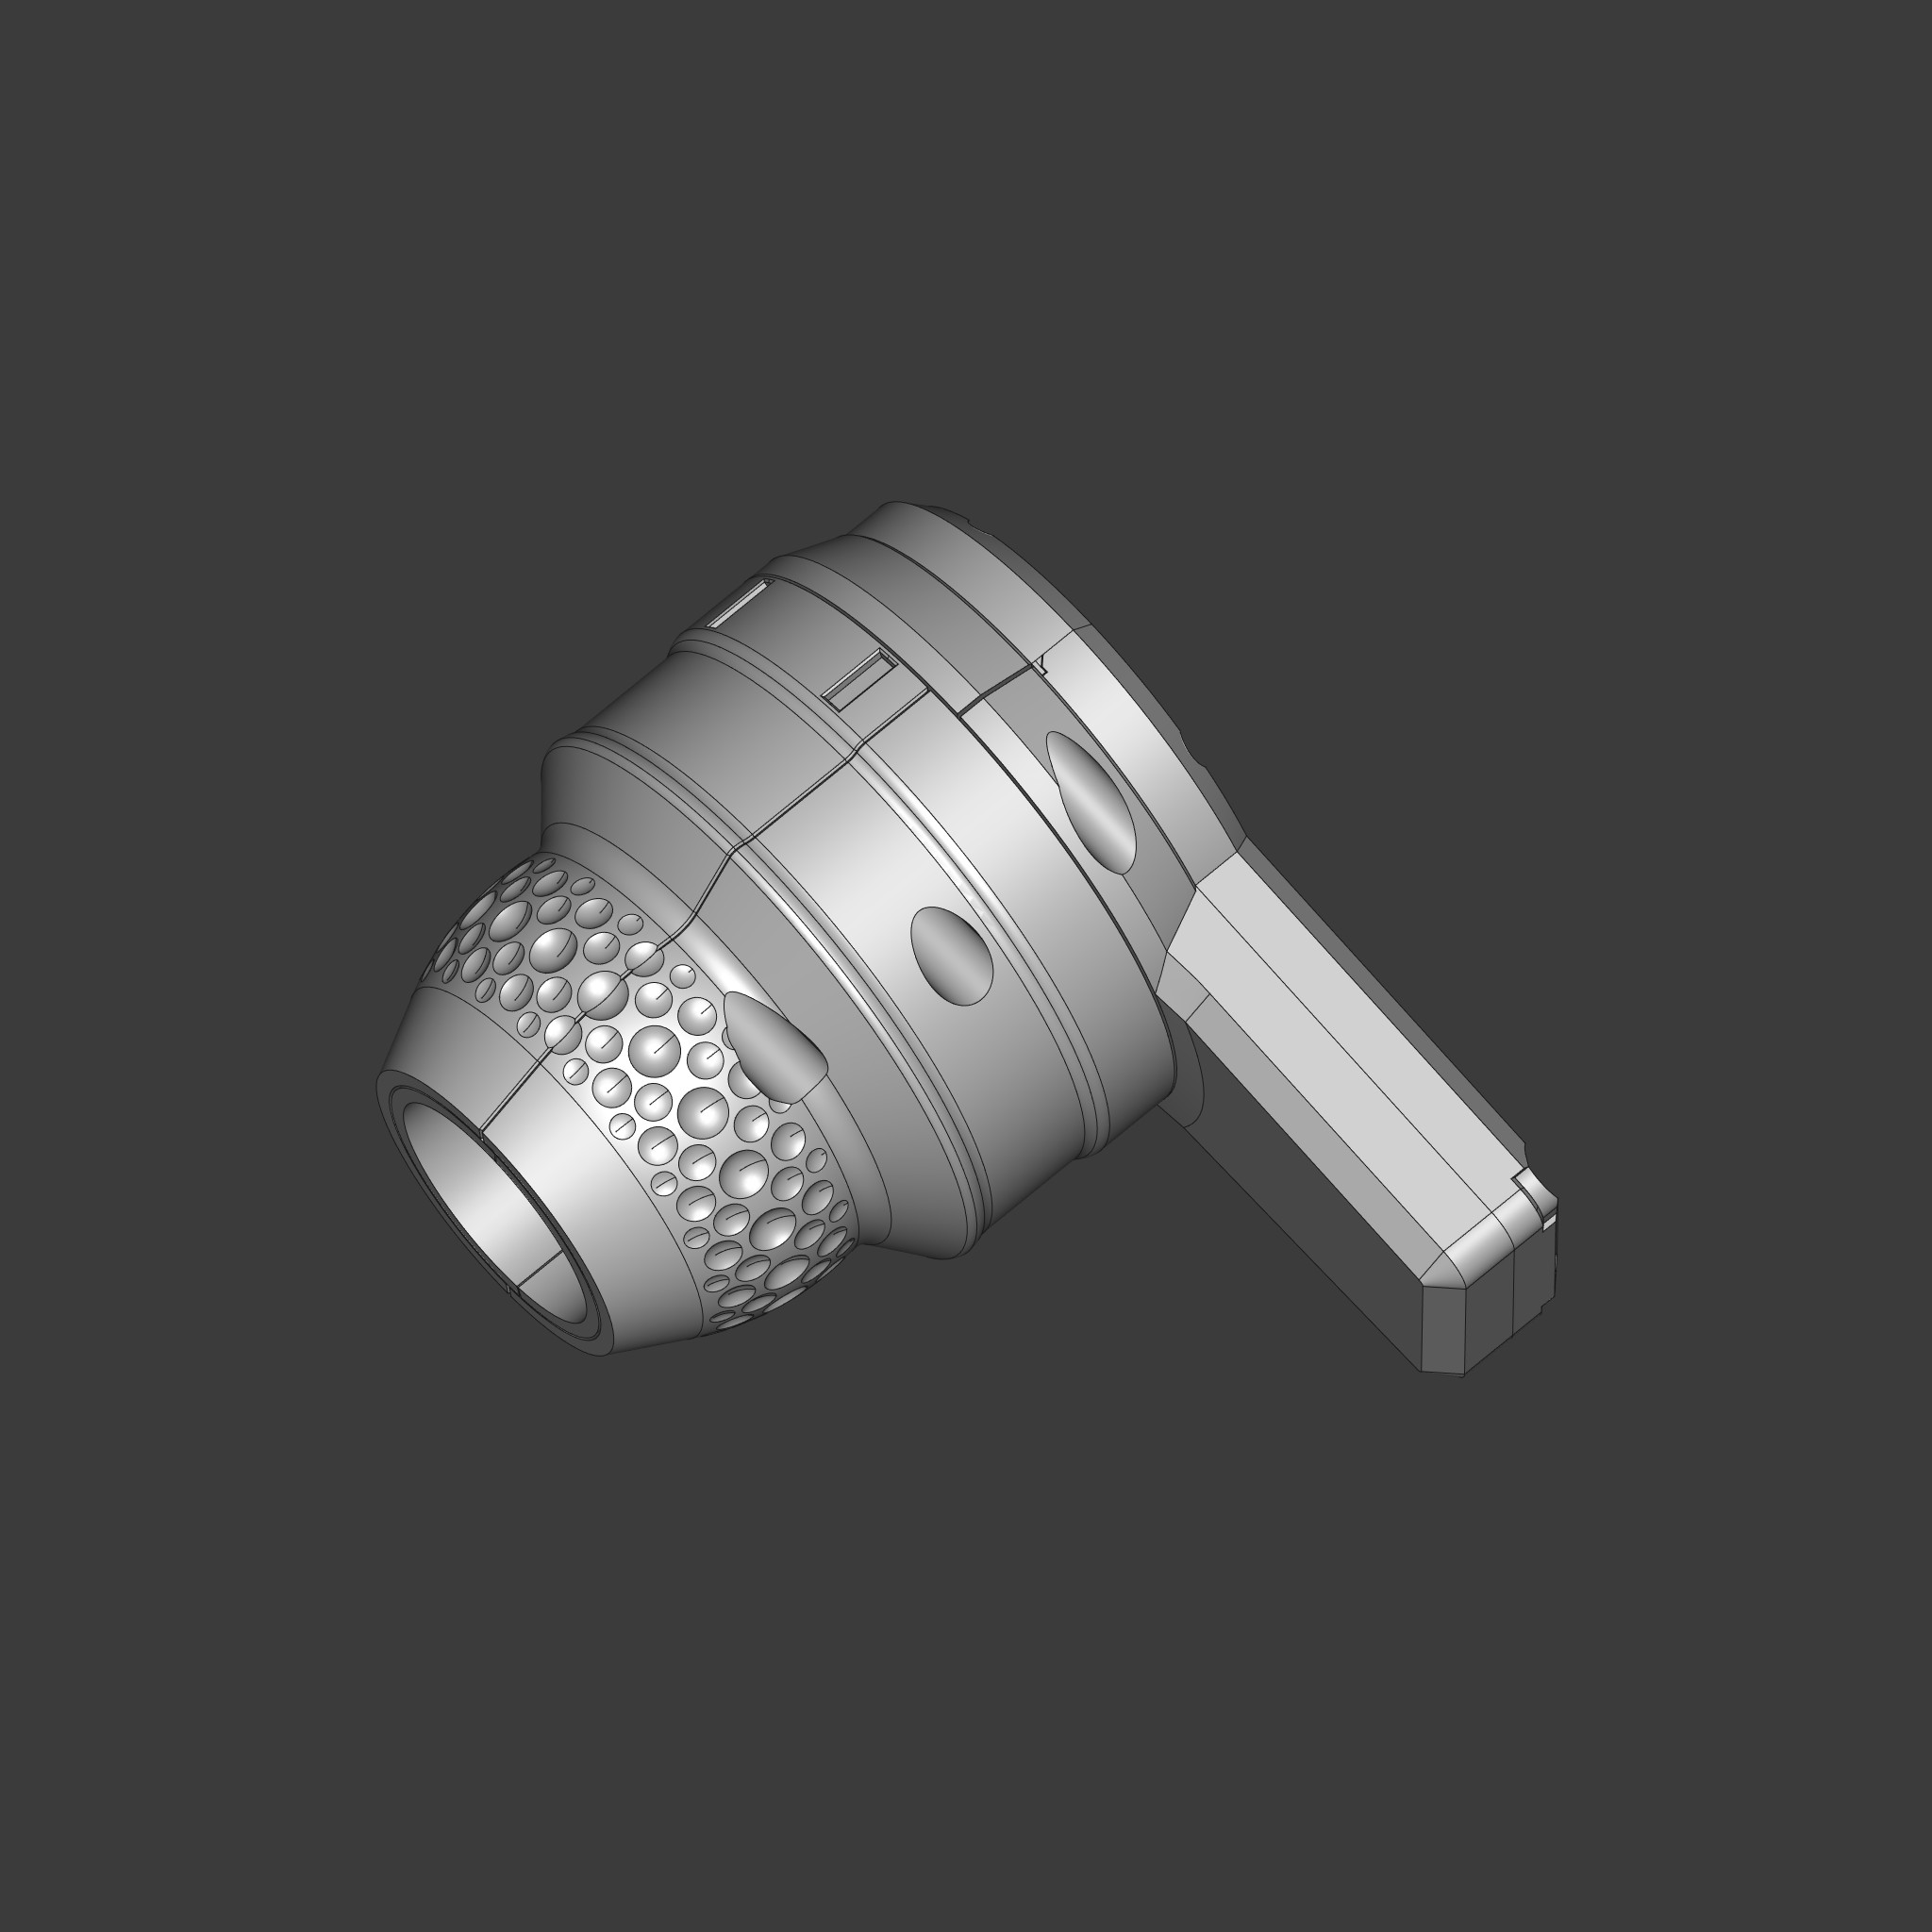
\includegraphics[width=.9\linewidth]{images/likertshift_freecad.jpg}
        \caption{CAD model}
    \end{subfigure}%
    \begin{subfigure}{.3333\textwidth}
        \centering
        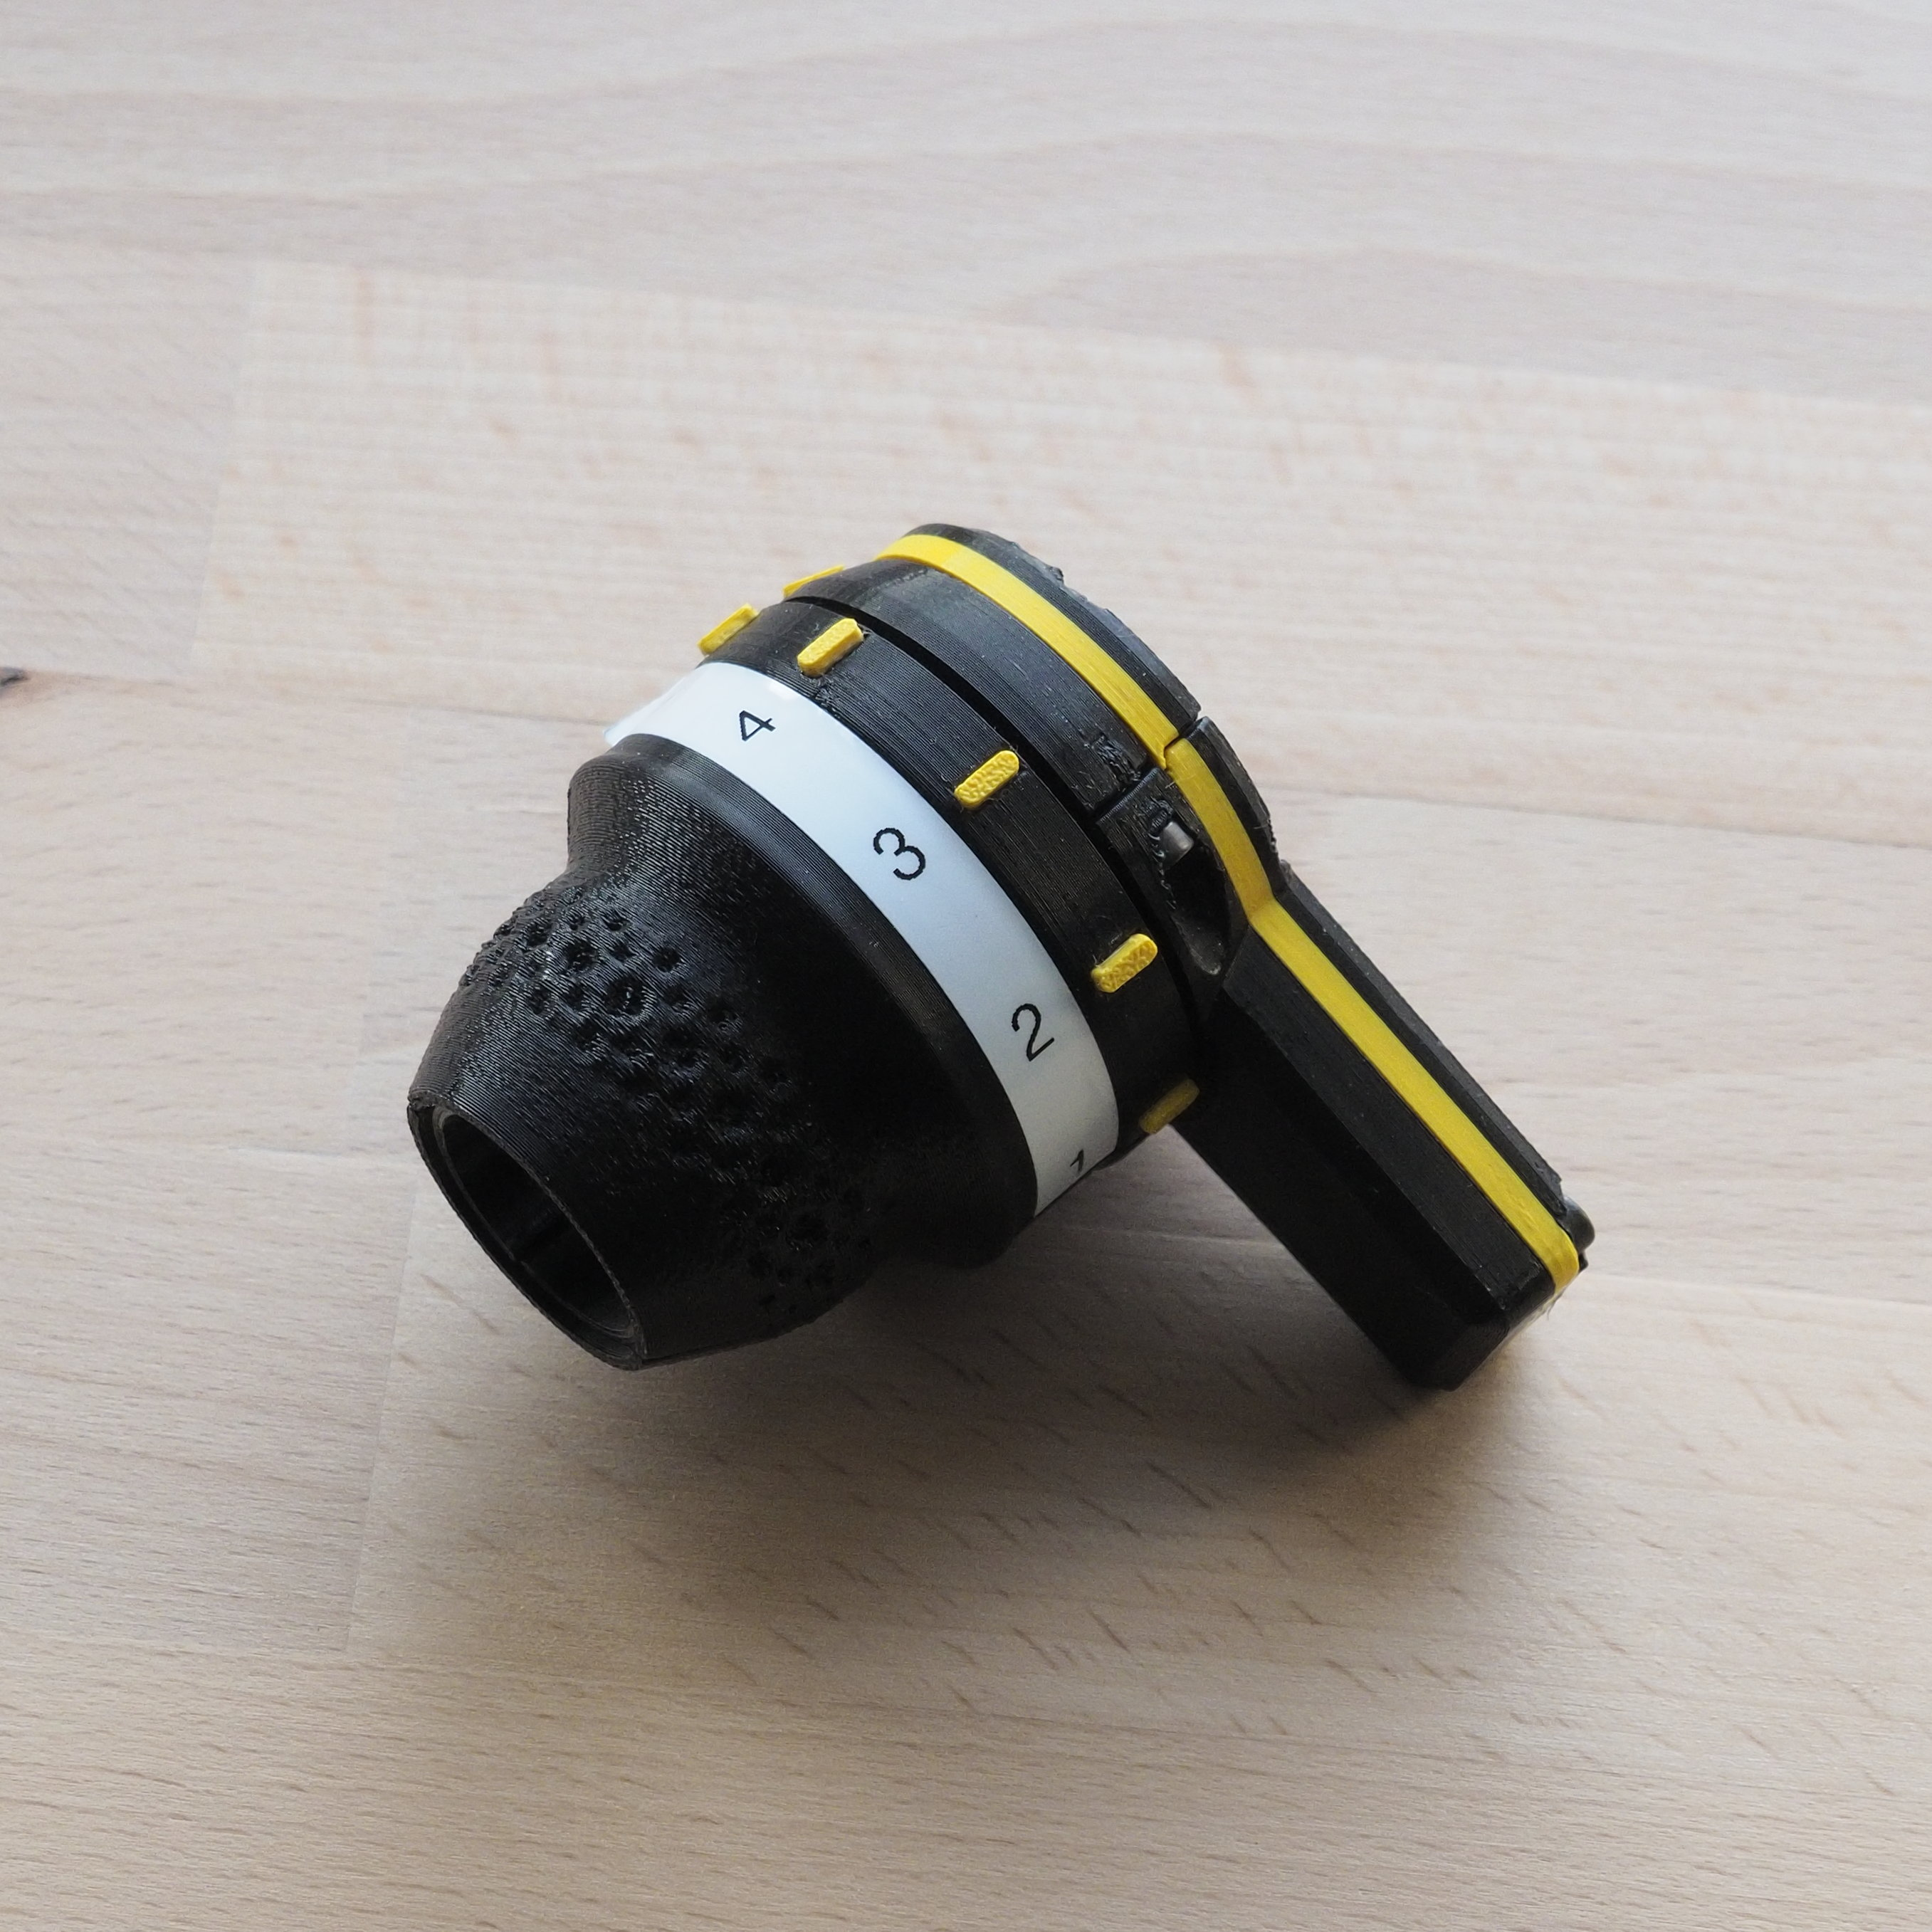
\includegraphics[width=.9\linewidth]{images/likertshift_assembled.jpg}
        \caption{Fully assembled}
    \end{subfigure}%
    \begin{subfigure}{.3333\textwidth}
        \centering
        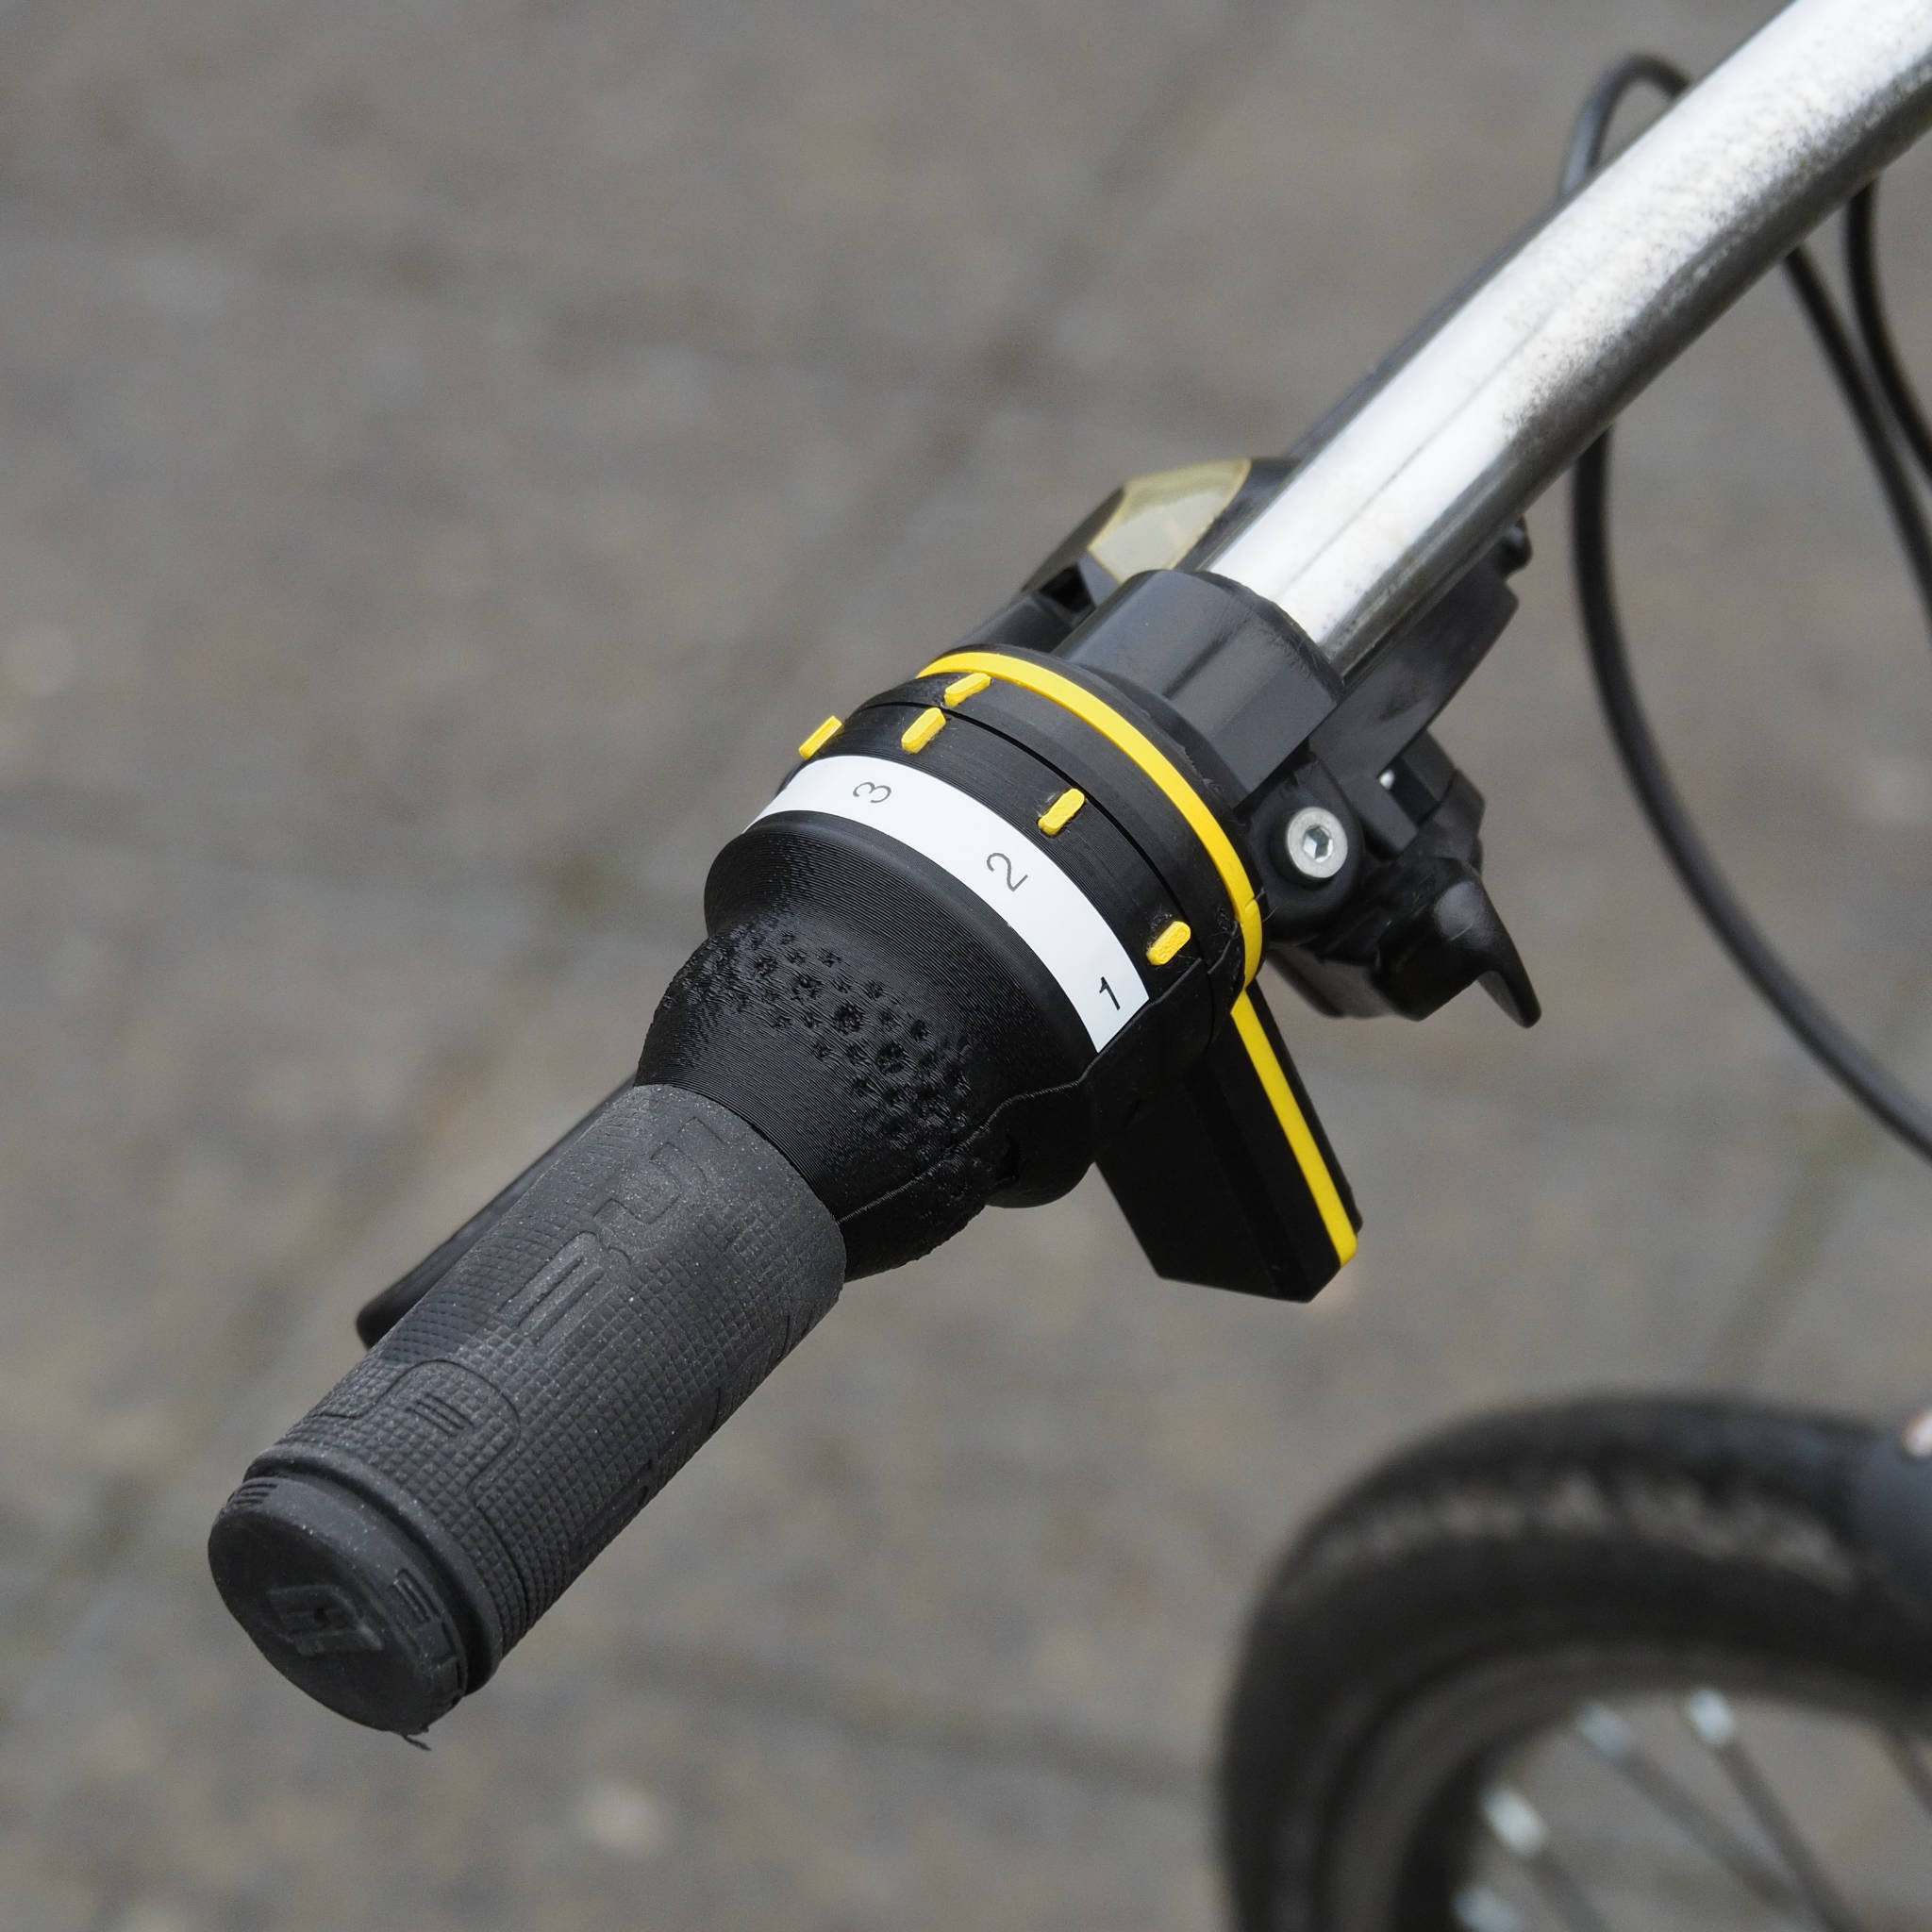
\includegraphics[width=.9\linewidth]{images/likertshift_mounted.jpg}
        \caption{Mounted to the handlebars}
        \label{subfig:likertshift_mounted}
    \end{subfigure}
    \caption{The final LikertShift prototype}
    \label{fig:likertshift}
\end{figure}

\noindent
To mount the prototype, the device is split in half and utilizes a simple clamping mechanism, similar to ones used for commercial bike accessories, to fix it to the handlebars.
We tried to add some texture to the clamping surface (see \autoref{subfig:cad_clamping_surface}), to reduce the necessary clamping pressure, but had mixed results with this.
The best solution to stop unwanted rotations and movements has been to apply a piece of masking tape to the handlebars at the desired mounting location.

We modeled a cavity to allow the application of a label sticker to mark the value of each discrete step and also added small markers to indicate the position that is currently selected.
The markers are 3D printed with a different filament color to improve visibility.
We also used a combination of CAD modeled indents, as well as the so-called “Fuzzy skin” feature in our slicer\footnoteurl{https://help.prusa3d.com/article/fuzzy-skin_246186} to add some texture to the grip area (see \autoref{subfig:slicer_textured_grip_area}).
This could be improved by utilizing multi-material 3D printing techniques and printing parts of it in more “grippy” materials like TPU, but we decided against such an approach, because multi-material 3D printing either requires special multi-toolhead printers or generates a lot of wasted material.

To satisfy \ref{drq:robust} and \ref{drq:easy_to_reproduce} we designed the device to be fully integrated, without requiring any external power.
\autoref{subfig:cad_pcb_compartment} shows the electronics compartment which houses the main Microcontroller board, as well as a button-cell battery to supply power to the electronics (see \autoref{subsec:electronics}).

\begin{figure}[!htb]
    \centering
    \begin{minipage}{.3333\textwidth}
        \centering
        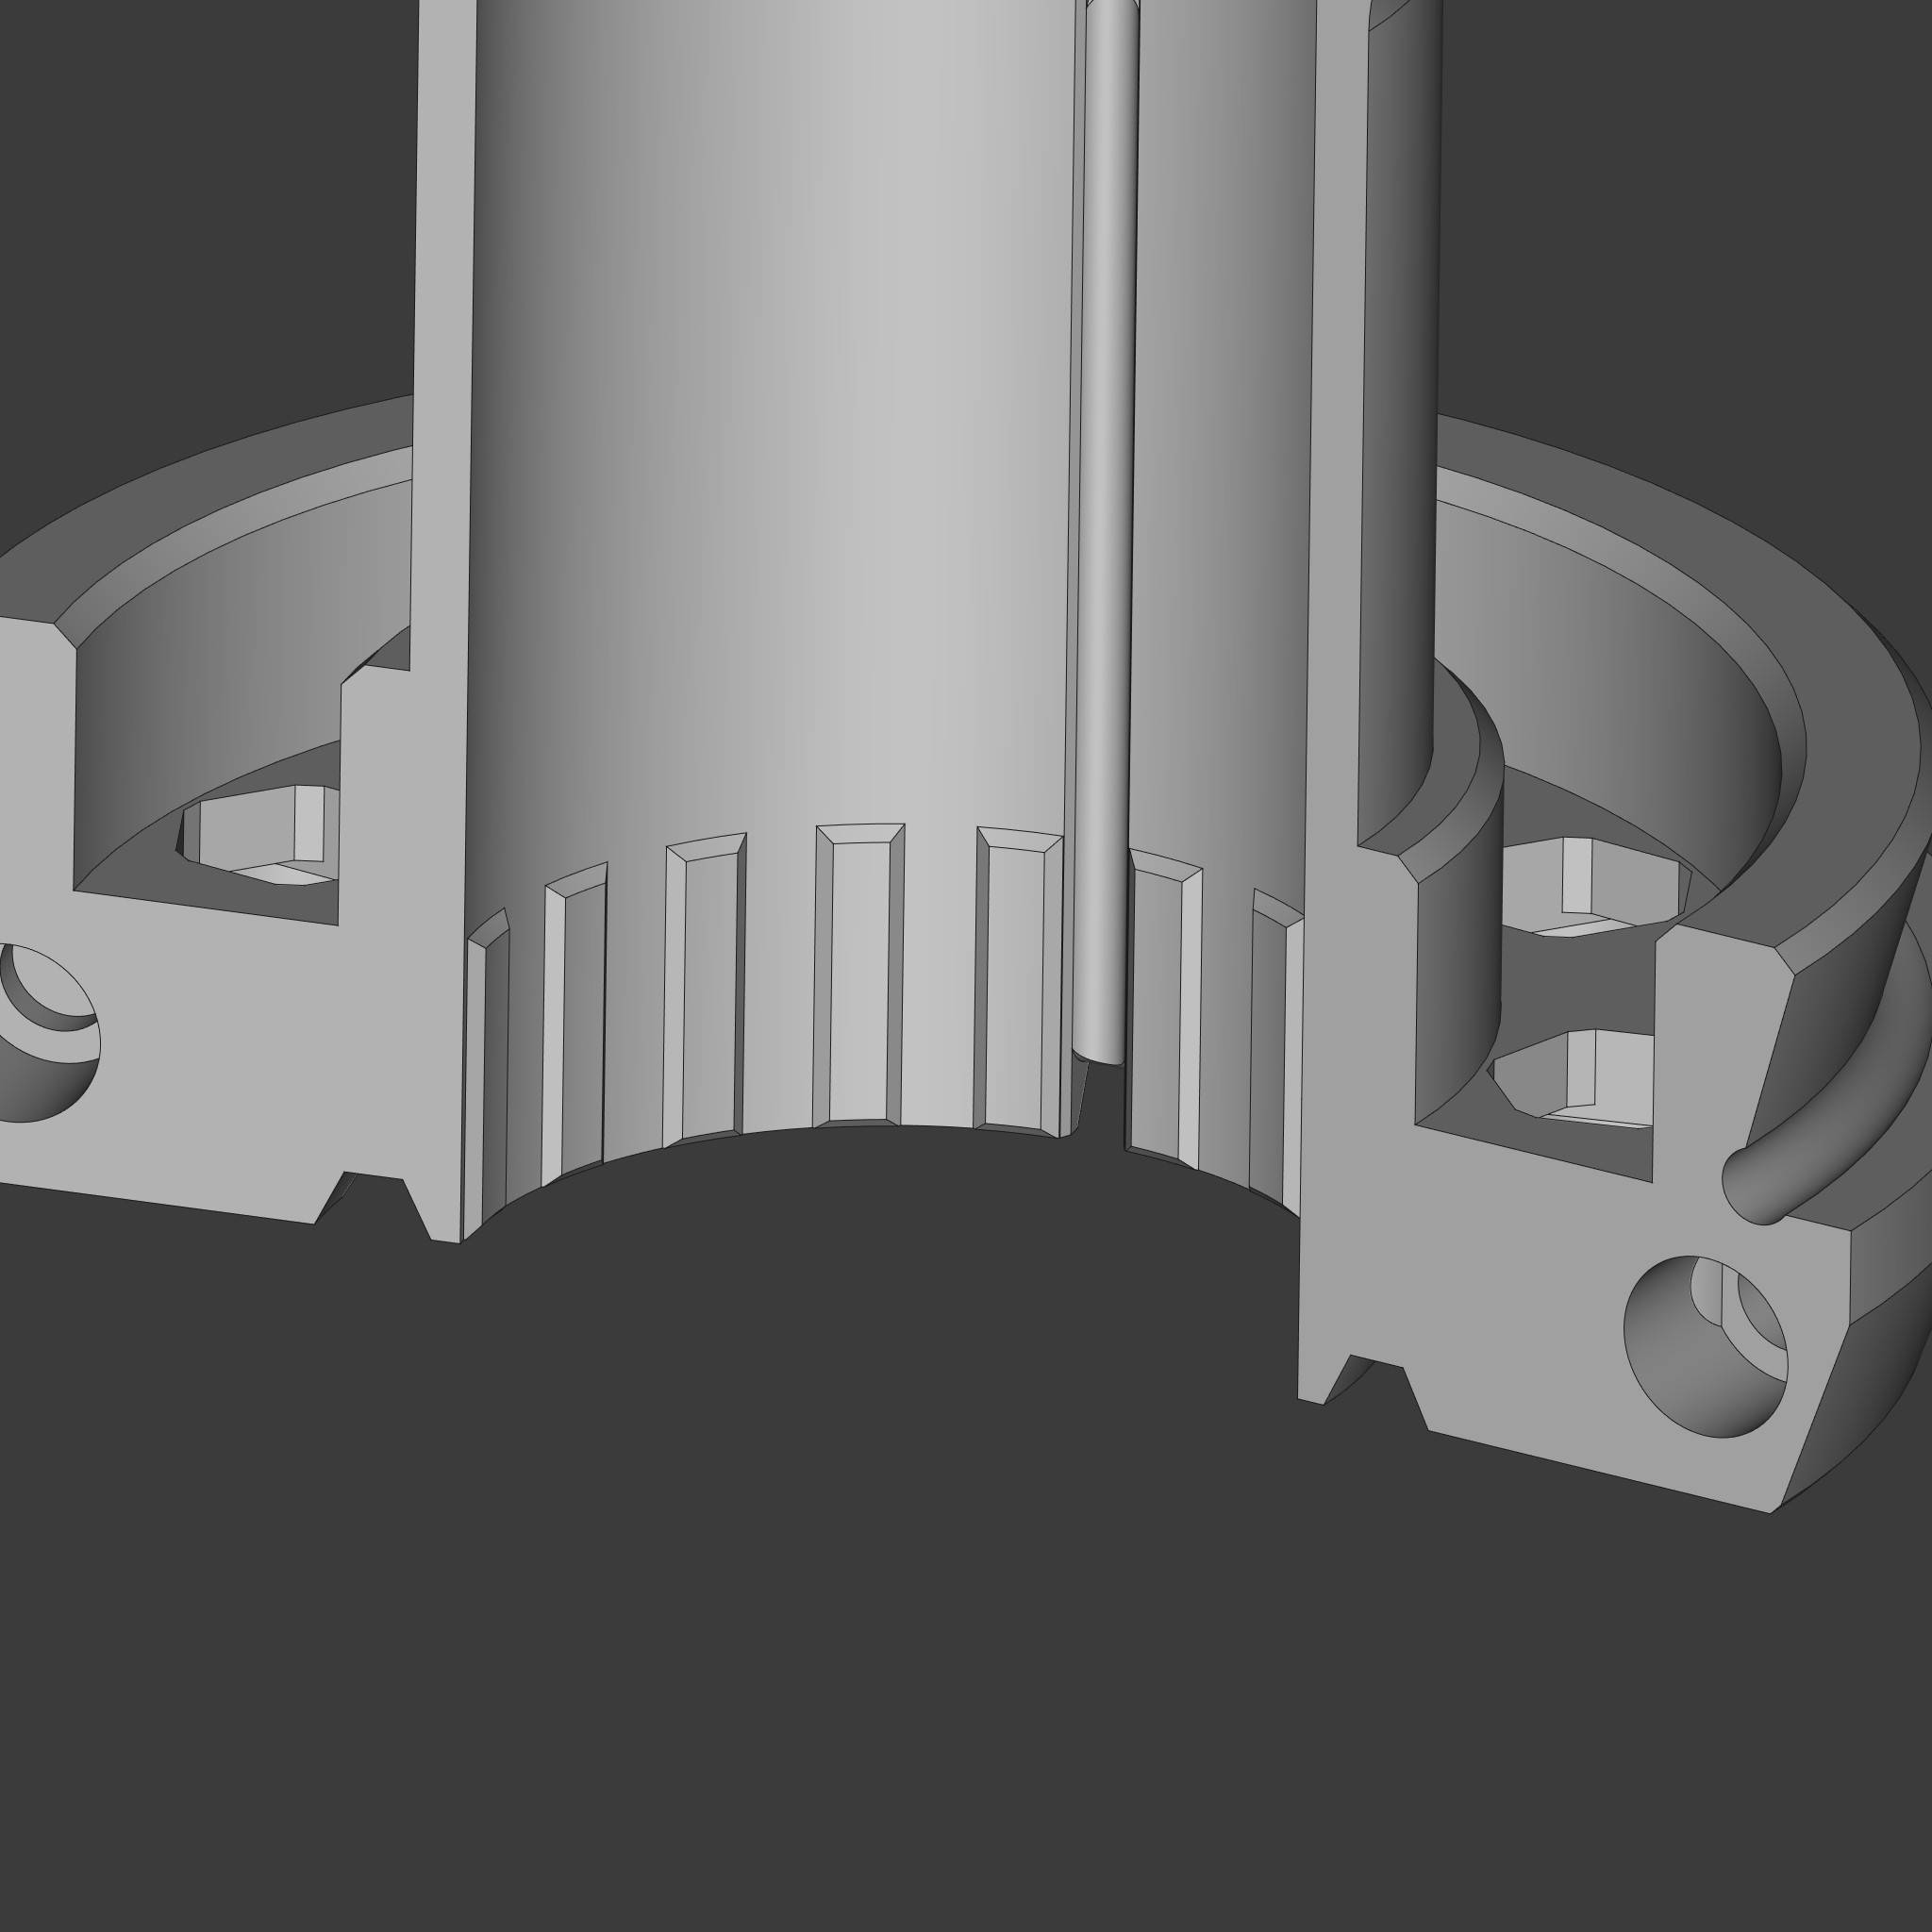
\includegraphics[width=.9\linewidth]{images/cad_clamping_surface.jpg}
        \caption{Clamping surface}
        \label{subfig:cad_clamping_surface}
    \end{minipage}%
    \begin{minipage}{.3333\textwidth}
        \centering
        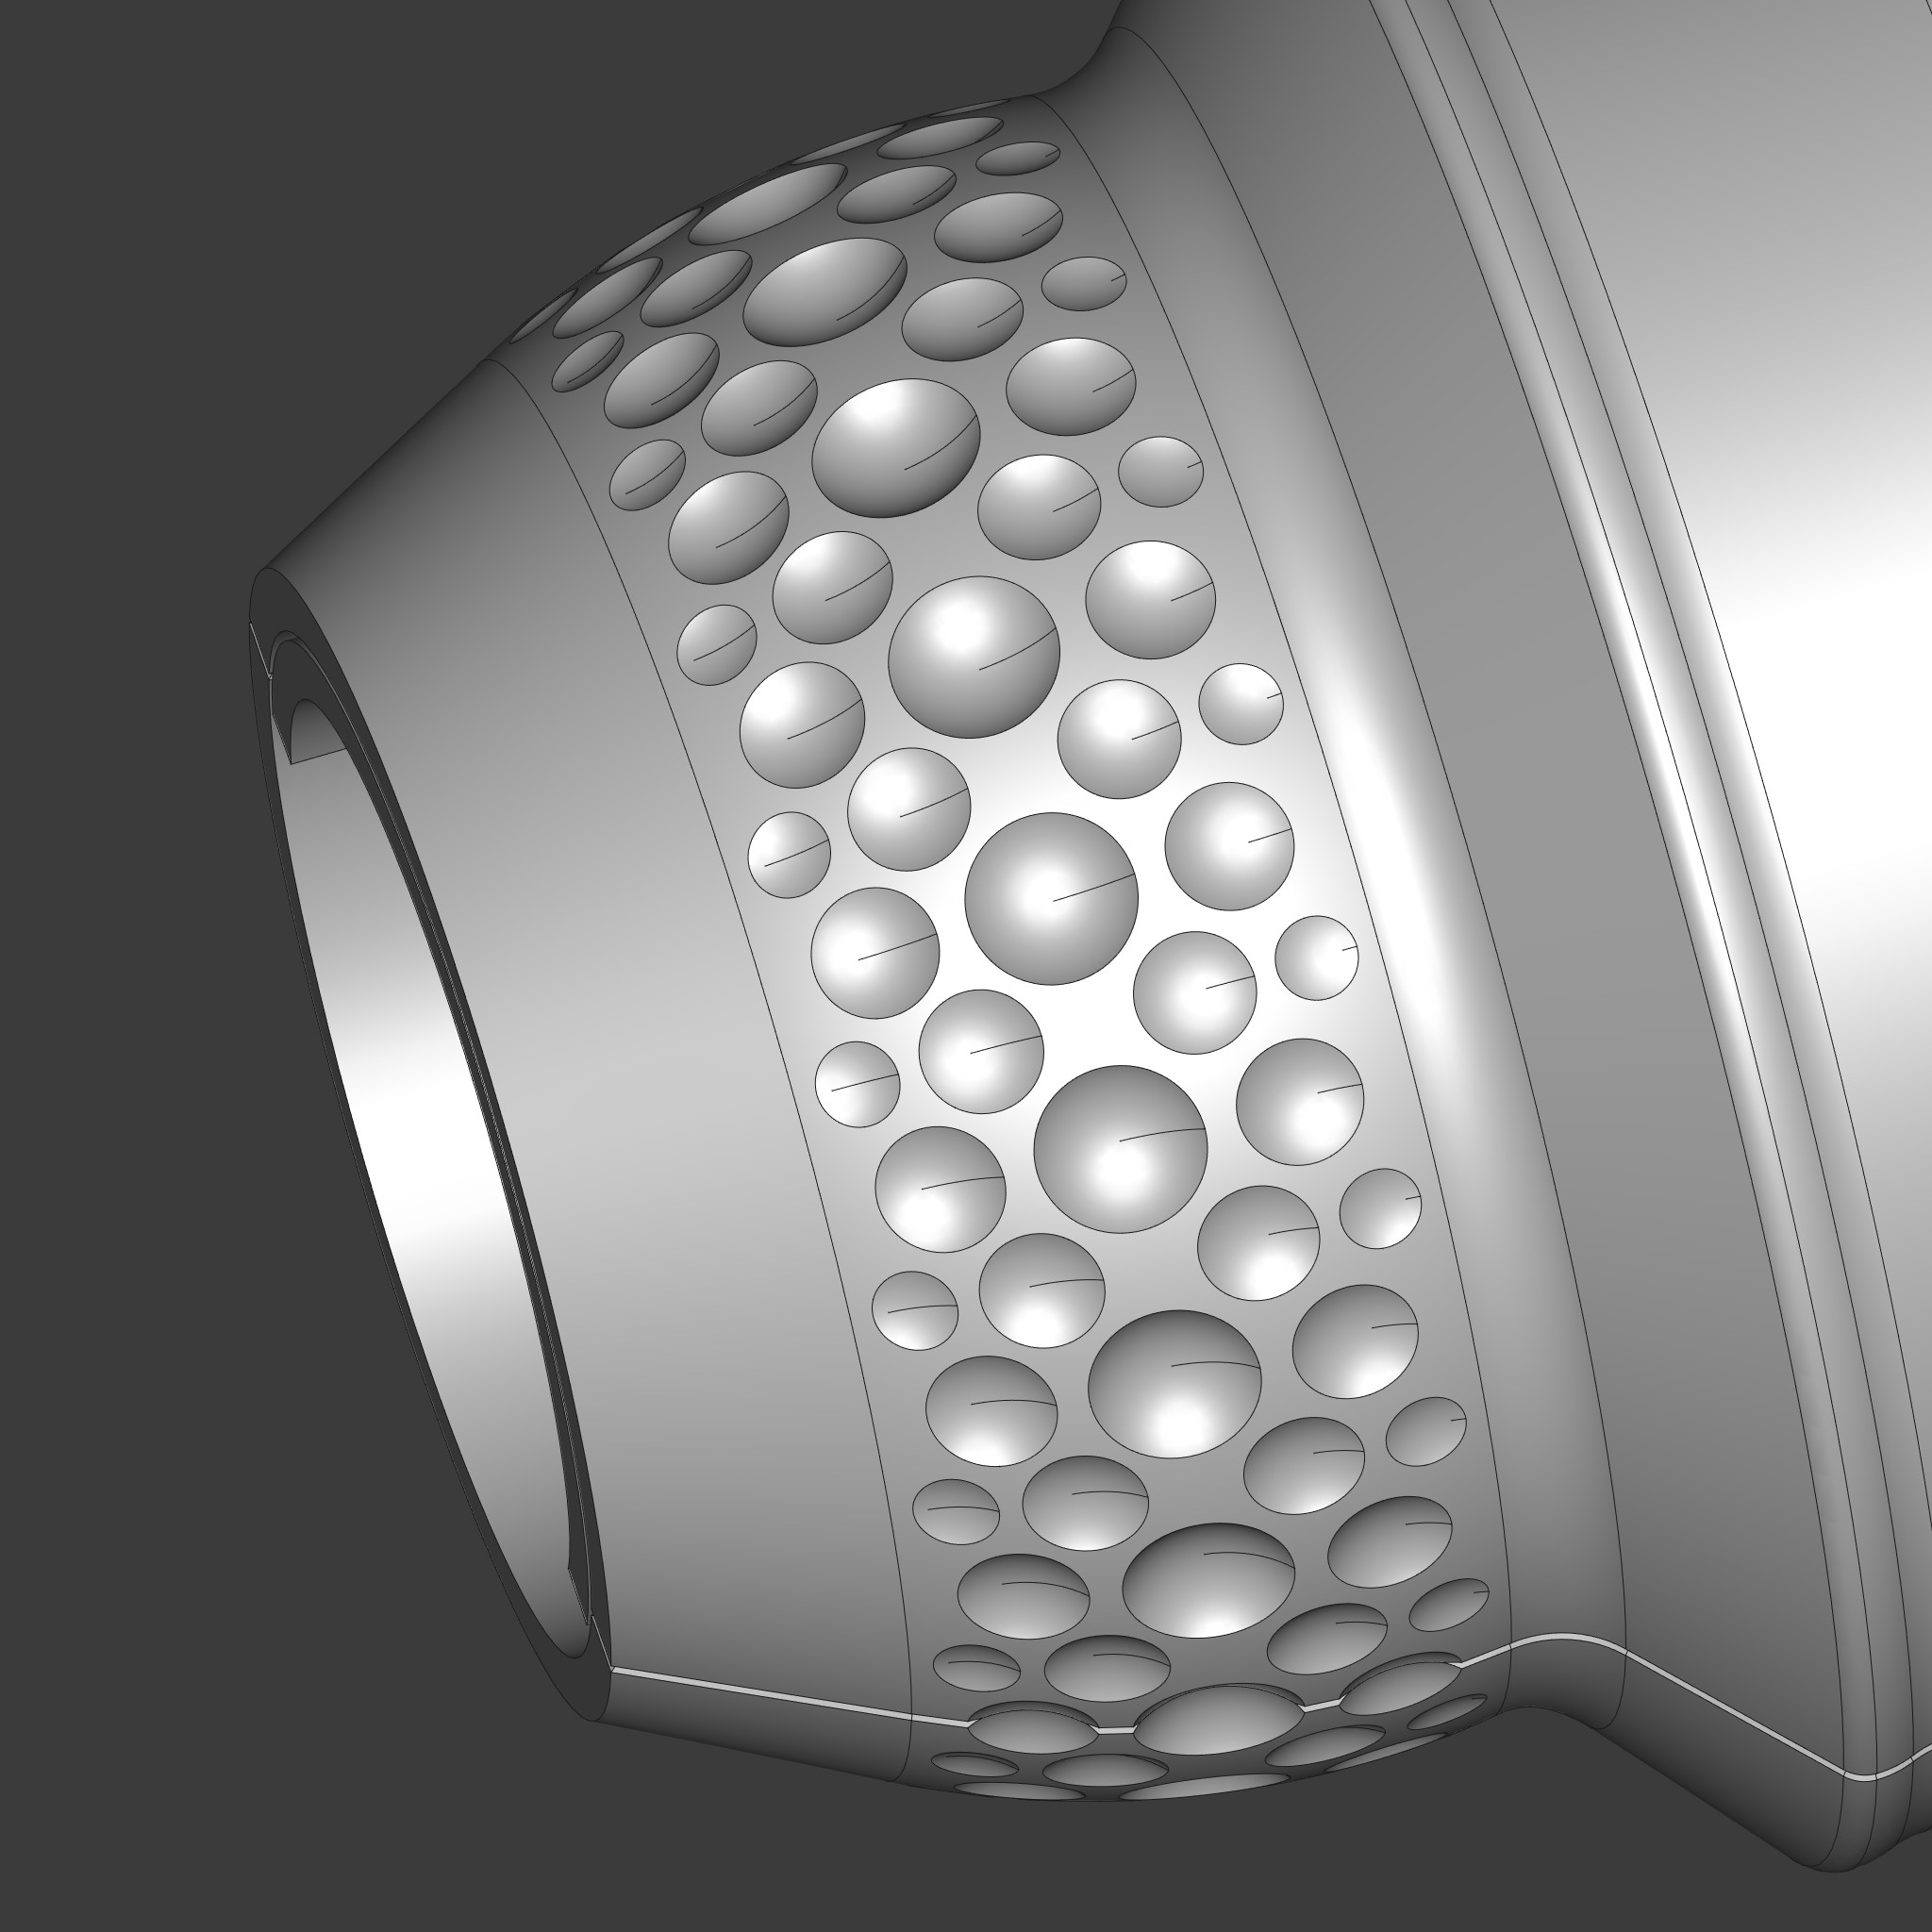
\includegraphics[width=.9\linewidth]{images/cad_grip_texture.jpg}
        \caption{Grip area}
        \label{subfig:slicer_textured_grip_area}
    \end{minipage}%
    \begin{minipage}{.3333\textwidth}
        \centering
        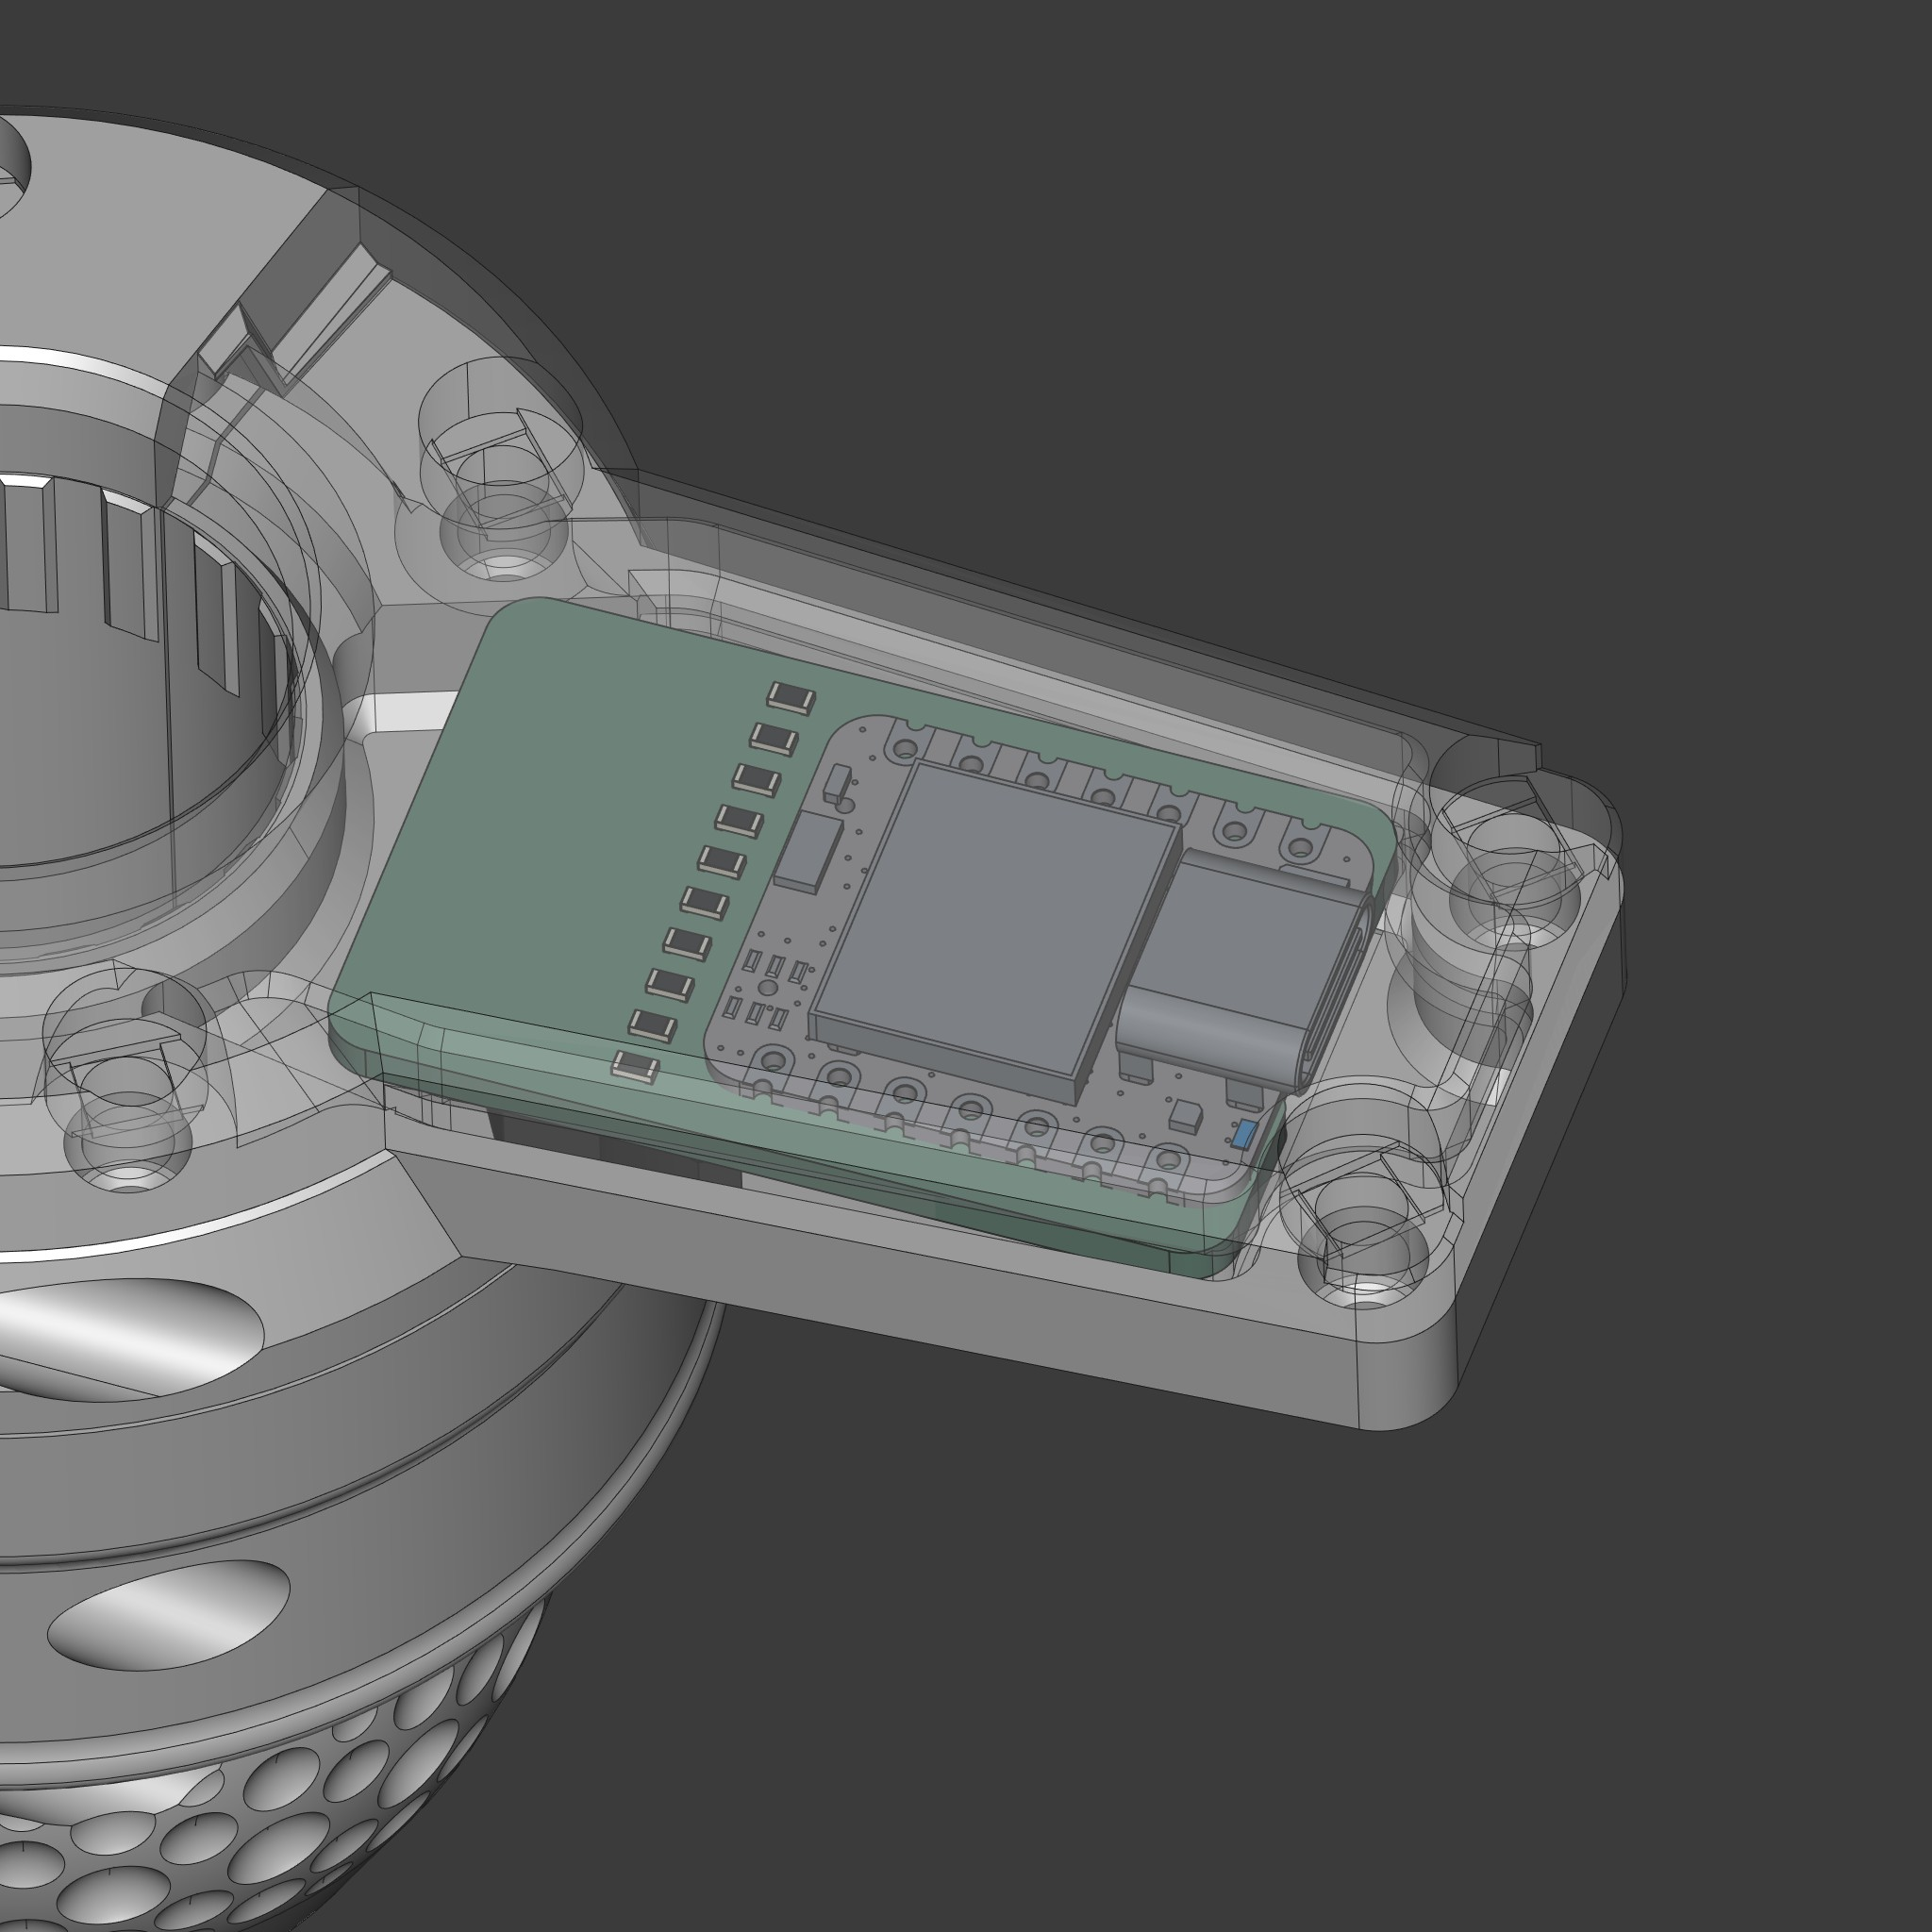
\includegraphics[width=.9\linewidth]{images/cad_pcb_compartment.jpg}
        \caption{PCB compartment}
        \label{subfig:cad_pcb_compartment}
    \end{minipage}
\end{figure}

\noindent
We used FreeCAD\footnoteurl{https://www.freecad.org/} (a parametric modelling software) in combination with OpenSCAD\footnoteurl{https://openscad.org/} (a code-based solid modelling software) for the mechanical design of our prototype. Both programs qualify as free and open-source software (FOSS), ensuring the design is accessible and modifiable by future contributors without requiring expensive software licenses.
The design was created parametrically, allowing for parameters like the number of discrete positions or their spacing to be easily adjusted.
All parts have been designed specifically for FDM 3D printing, with a particular print orientation in mind and don't require any additional support structures when printing.

\subsubsection{Mechanism}\label{subsec:mechanism}

\def\rotator{\textsf{Rotator}\xspace}
\def\rotatorhead{\textsf{Rotator-head}\xspace}

The prototype uses a simple rotary switching mechanism.
When the outer \rotator gets rotated, it pulls the \rotatorhead along a ramped track (see \autoref{fig:cad_ramped_track}).
The \rotatorhead, shown in \autoref{fig:cad_rotator_head}, consists of a \SI{4}{mm} steel bearing ball that is socketed into a 3D printed part and gets pushed into the track by a spring.
It is constrained to only move along the rotation axis by $\sim\SI{5}{\mm}$ to be able to overcome the ramps.
This way, the mechanism automatically snaps into the depressions between the ramps.

At the bottom of the depressions are nickel-plated neodymium magnets which are being used as the switching contacts while the \rotatorhead acts as the contactor.
M3 button head screws are used to clamp and connect cables to the contactor and switching contacts.
As the cable that goes to the \rotatorhead experiences lots of movement and thus relatively high stress, we used special FEP insulated wire\footnoteurl{https://shop.helukabel.com/de-en/heluflon-fep-6y-m25511/20271} made for the use in cable chains for it.
For the contacts we used standard PVC insulated wire.
This setup results in a total contact resistance of $\sim\SI{10}{\ohm}$, which is well within useable range for our purposes.

\begin{figure}[!htb]
    \centering
    \begin{minipage}{.3333\textwidth}
        \centering
        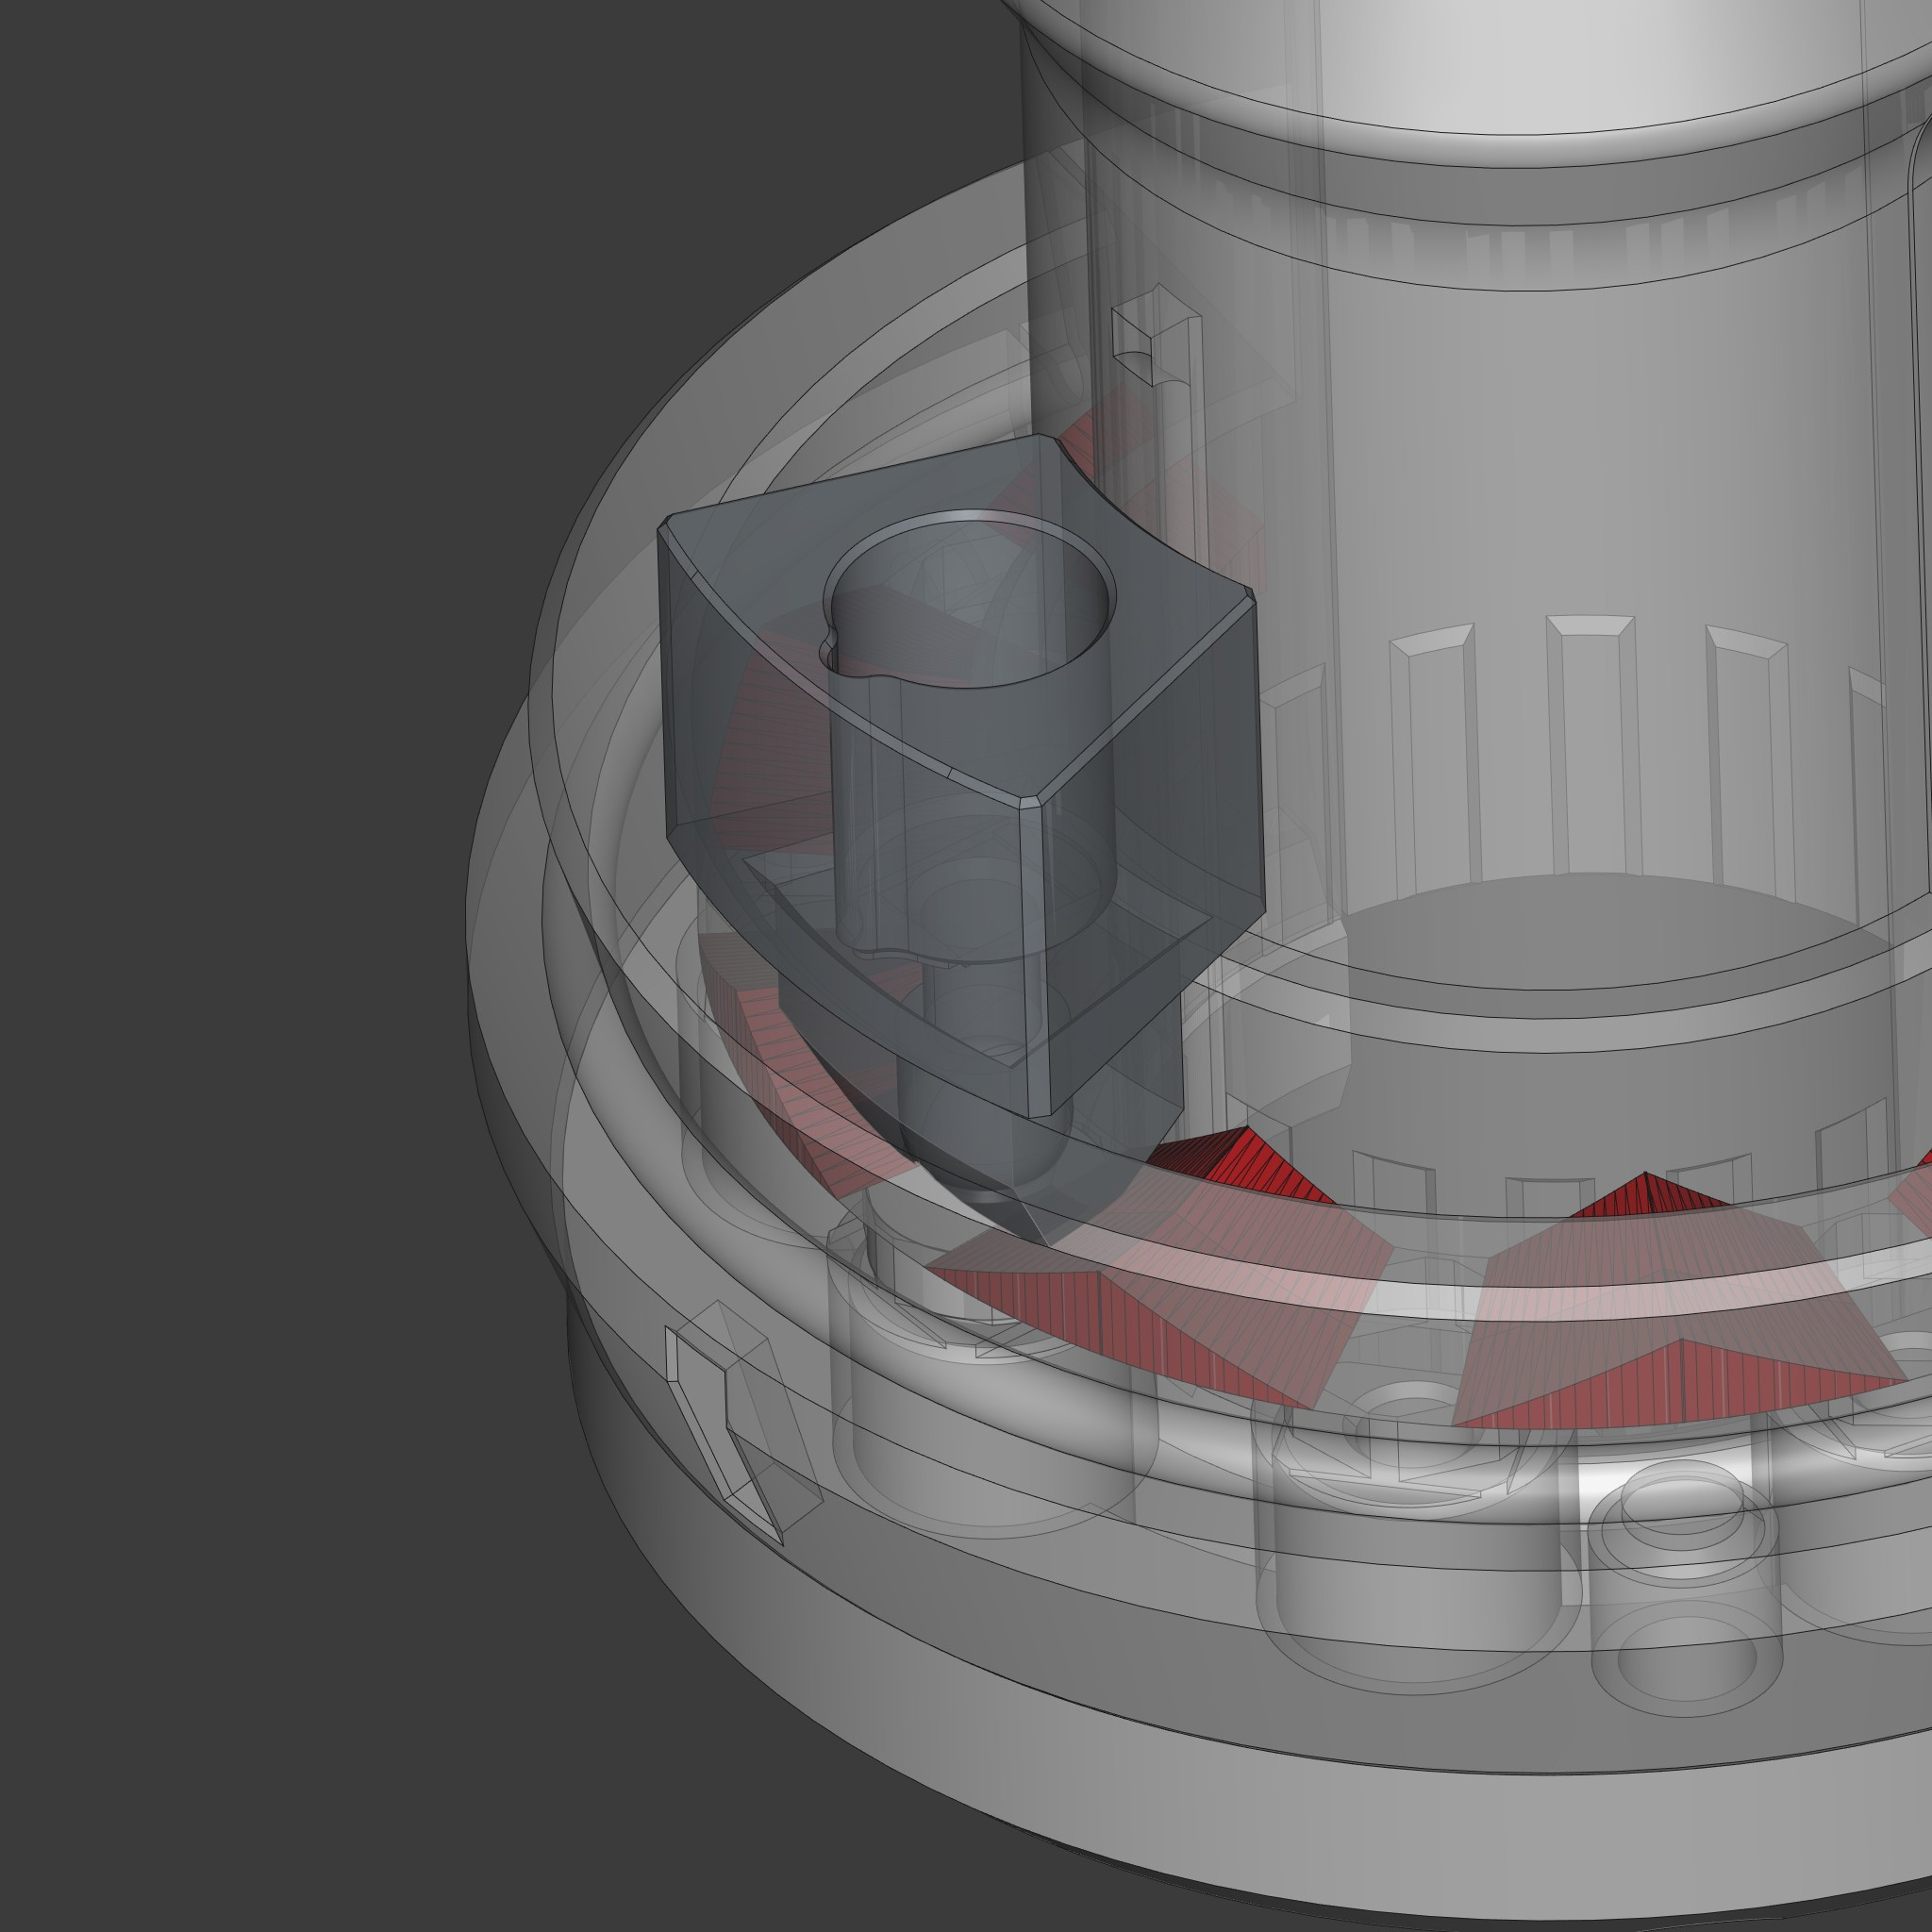
\includegraphics[width=.9\linewidth]{images/cad_ramped_track.jpg}
        \caption{Ramped track}
        \label{fig:cad_ramped_track}
    \end{minipage}%
    \begin{minipage}{.3333\textwidth}
        \centering
        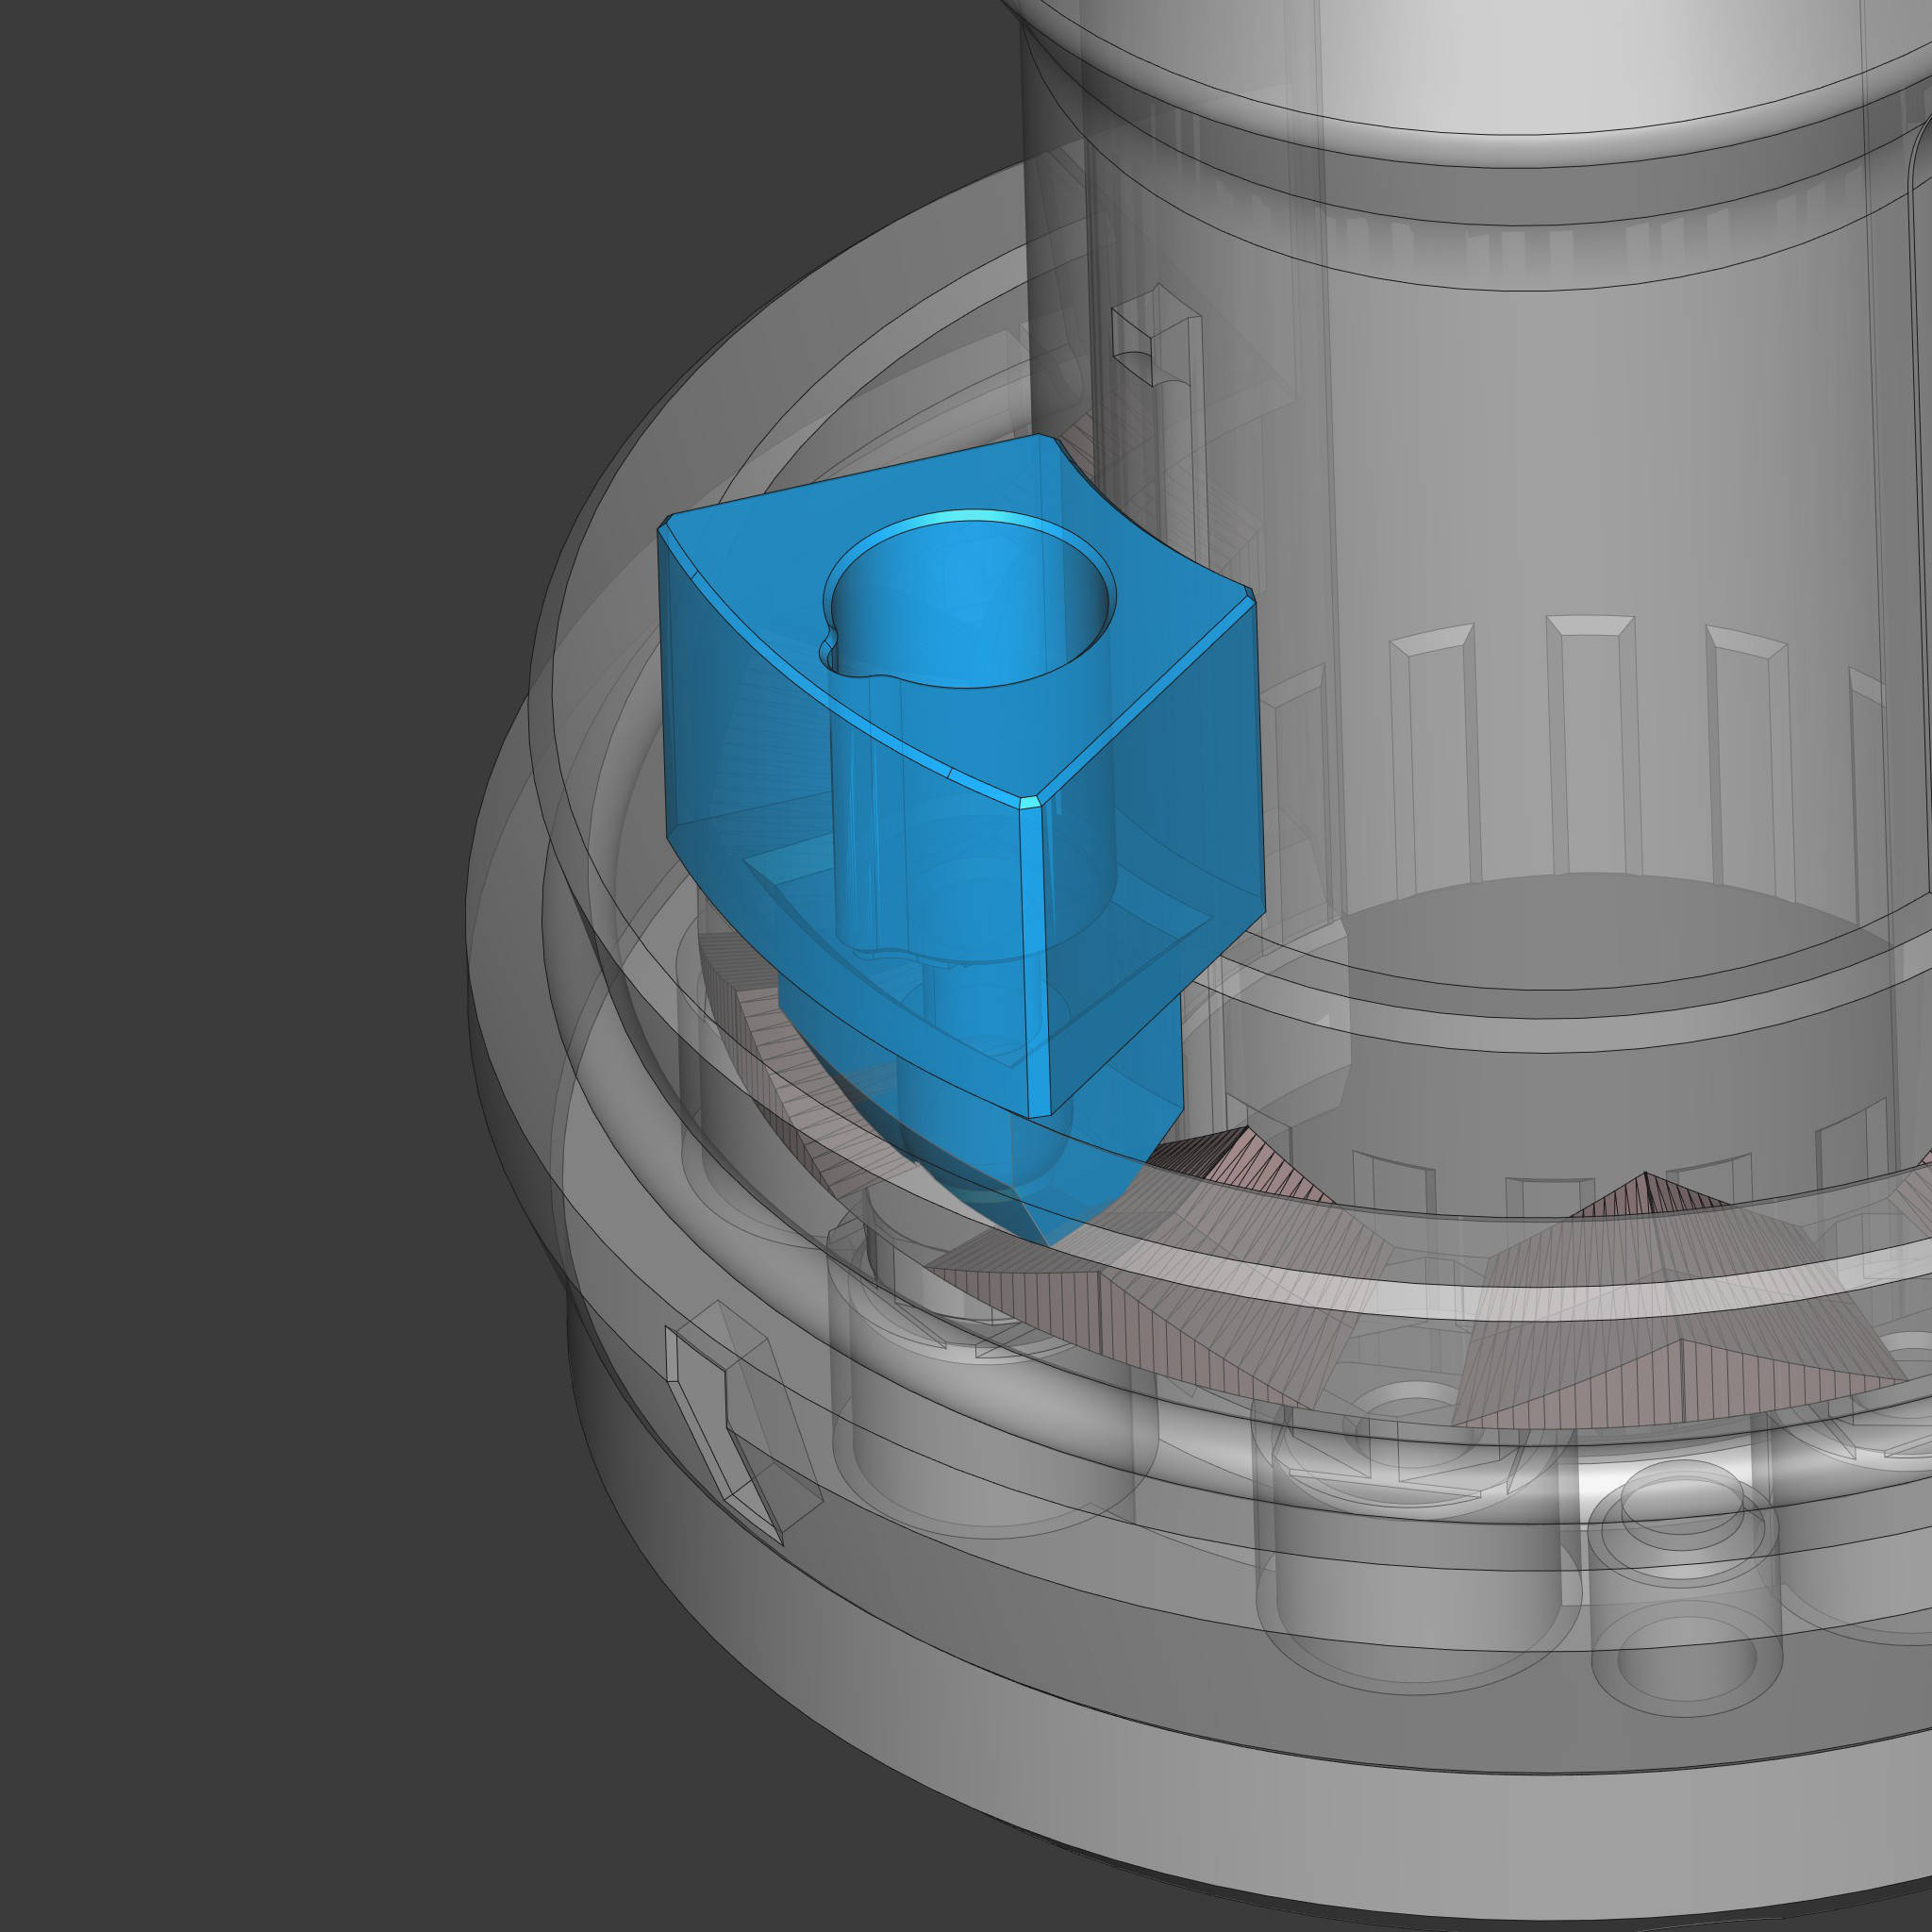
\includegraphics[width=.9\linewidth]{images/cad_rotator_head.jpg}
        \caption{\rotatorhead}
        \label{fig:cad_rotator_head}
    \end{minipage}%
    \begin{minipage}{.3333\textwidth}
        \centering
        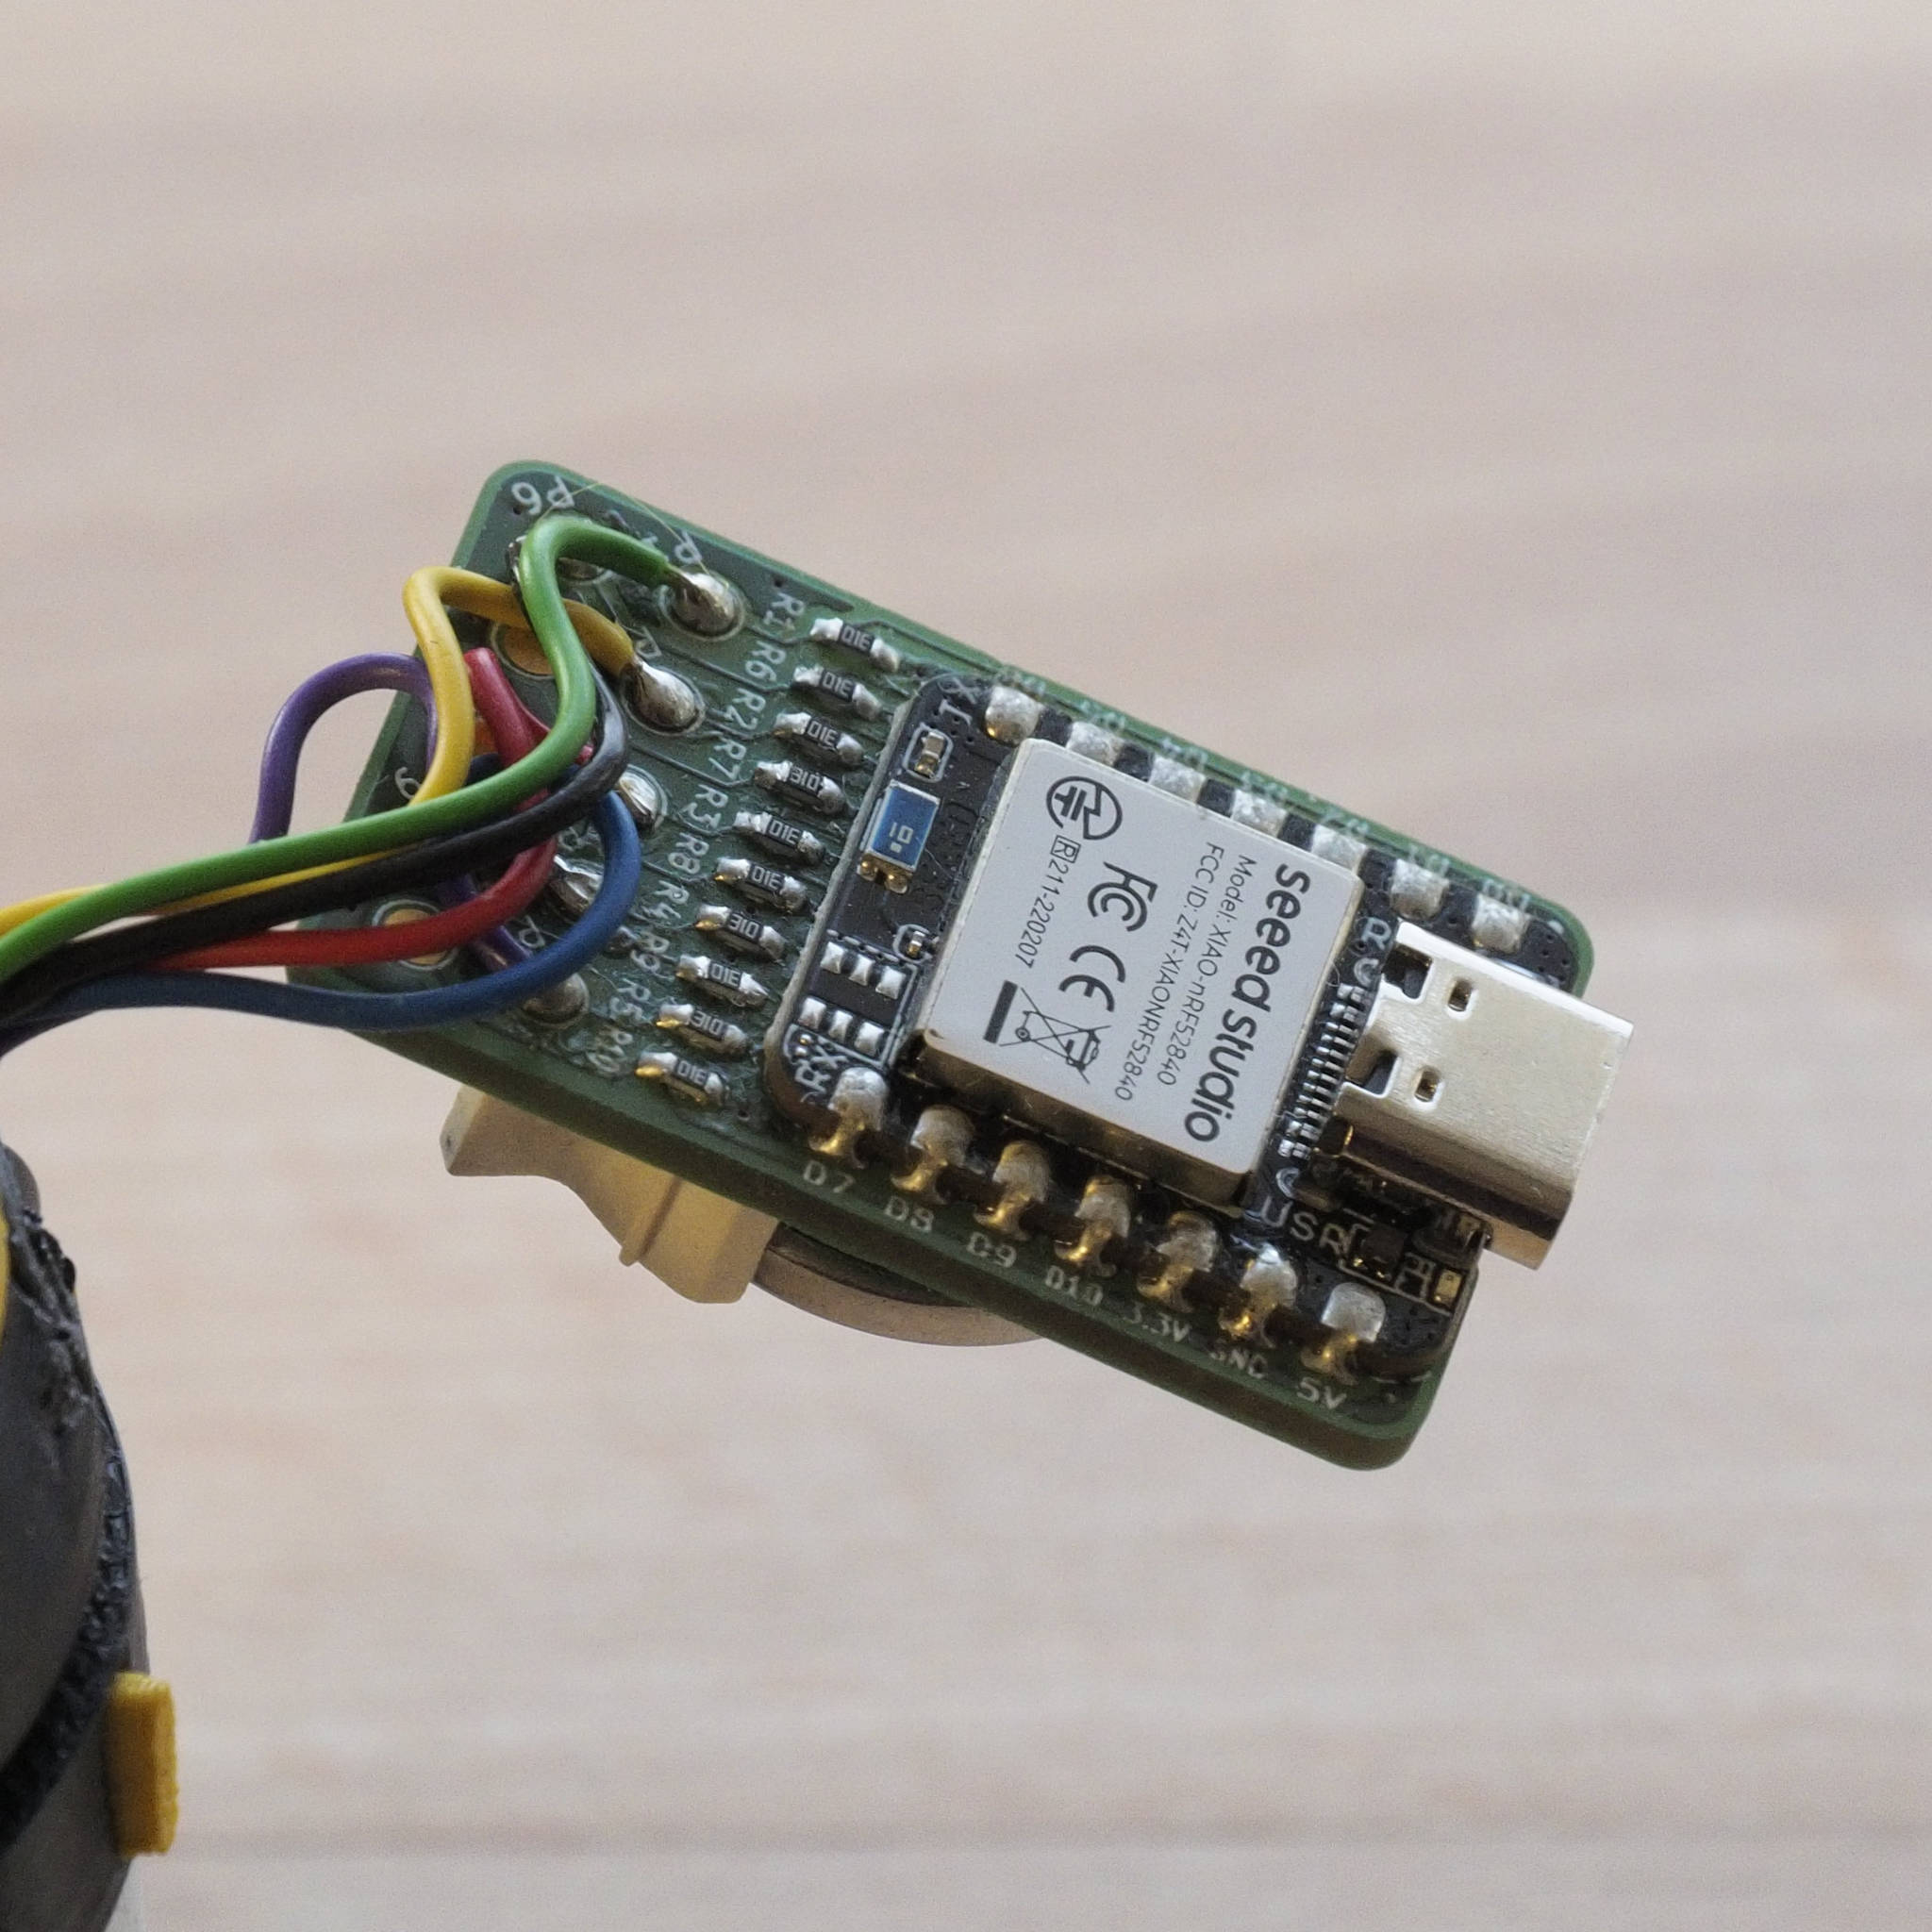
\includegraphics[width=.9\linewidth]{images/likertshift_pcb.jpg}
        \caption{Assembled PCB}
        \label{fig:likertshift_pcb}
    \end{minipage}
\end{figure}

\noindent

\subsection{Electronics}\label{subsec:electronics}

This section describes our electronics design, as well as microcontroller choice and power requirements.
For retrieving data from the prototype to our frontend (see \autoref{subsec:frontend_design}), we decided to use the Bluetooth Low Energy (BLE) network, as it offers low-power operation, is supported by most modern smartphones and does not require stationary access points to function.
We also only need very short-range communication capabilities, as the user is always situated right next to our device.

\subsubsection{Microcontroller Choice}

For data acquisition and communication we wanted to use the nRF52 series Microcontroller Units (MCUs) because of their exceptionally low-power usage, Bluetooth Low Energy (BLE) capabilities and wide availability\footnoteurl{https://docs.nordicsemi.com/category/nrf-52-series}.
Specifically, for our prototype we decided to use a relatively affordable (\ref{drq:affordable}) nRF52840 based development board by Seeed Studio\footnoteurl{https://wiki.seeedstudio.com/XIAO_BLE/}.
Using a development board allowed us to skip many electrical design challenges and to test the working principle of our prototype on a solderless breadboard.

\subsubsection{Power}

To satisfy \ref{drq:robust} and \ref{drq:easy_to_reproduce} we designed our device to be fully integrated and enclosed.
Due to the given space-constraints by our mechanical design it is only powered by a standard CR2032 button cell battery.
Under optimal conditions, it should be able to power our device for at least 1--2 years.
We did not optimize our firmware to achieve this kind of power usage though (see \ref{subsec:firmware}).

\subsubsection{Printed Circuit Board (PCB)}

To minimize wiring and to keep the electronics tightly integrated, we designed a simple breakout-PCB (see \autoref{fig:likertshift_pcb}) that holds the MCU development board and a battery holder and exposes solder pads that allow easy connection of the contactors described in \ref{subsec:mechanism}.
The solder pads allow connecting of up to ten such contactors, so it can be used with variants of the device with up to nine discrete positions.
The solder pads connect directly to the MCUs' General-Purpose Input/Output (GPIO) pins, as well as a high-impedance pull-down resistors to hold the logic state to $0V$ when not in use.

The two-layer PCB design was implemented using the KiCad Electronics Design Automation Suite (KiCad EDA) and is optimized for affordable manufacturing with design rules allowing for comparably high production tolerances.
The KiCad EDA also qualifies as FOSS.

\subsubsection{Firmware}\label{subsec:firmware}

\def\gpiohigh{\texttt{HIGH}\xspace}

When powered up, the prototype starts to advertise itself via BLE, broadcasting its name and that it is ready to accept connections.
Once a central device, the smartphone in our case, initiates a connection, the prototype hosts a Generic Attribute (GATT) server providing two services, a custom \likertshift service to retrieve the currently selected switch position and a battery service to retrieve the current battery level.
Both services each offer a one-byte characteristic that can be read by the central device.

When the \likertshift characteristic gets read, first the GPIO pin connected to the contactor at the \rotatorhead gets set to a \gpiohigh state ($\sim\SI{3.3}{V}$) then each of the pins connected to the switching contacts gets read, checking for a matching \gpiohigh state.
Finally, the detected position gets sent back to the central device, as a value from \mbox{$1$ -- $n_{positions}$}.
There are two special cases here:
\vspace*{-0.5em}
\begin{enumerate}[label=(\roman*),itemsep=0em]
    \item No switching contact is set to a \gpiohigh state.\\
        This can happen if the service gets read while the prototype is currently being moved from one position to another. In this case the service will return a value of $0$. How exactly this state should be handled is left to the software running of the central device.
    \item Multiple switching contacts are set to a \gpiohigh state.\\
        This should not happen during normal operation. In this case the service returns the position corresponding to the last GPIO pin read.
\end{enumerate}
\vspace*{-0.5em}
\noindent
When the battery characteristic gets read, the battery voltage is measured by the MCUs onboard Analog to Digital Converter (ADC).
Then, the measured voltage gets linearized and scaled to a value from $0$ -- $255$ and sent back to the central device.

\bigbreak\noindent
The firmware is written in Rust\footnoteurl{https://www.rust-lang.org/} using Embassy\footnoteurl{https://embassy.dev/} (a framework for embedded applications).

\newpage
\subsection{Frontend Design}\label{subsec:frontend_design}

To view and record ratings using the \likertshift we need a frontend that can connect to it via BLE and talk to our firmware to retrieve the currently selected position.
Because we also want to record location data simultaneously and the \likertshift hardware does not possess GPS recording capabilities, we decided to implement this frontend as a smartphone app.
This way, we can also extend it to query other information, relevant for our evaluation, from study participants.

\subsubsection{Features}

The base implementation of the app allows users to:

\begin{itemize}[itemsep=0em]
    \item connect to nearby \likertshift devices and display their currently selected rating.
    \item record GPS locations and \likertshift ratings along arbitrary travel routes.
    \item view their current location and travelled route on a 2D map.
\end{itemize}

\noindent
We later extended the app for performing our own field-study.
We took great care to make it as customizable and reusable as possible, so other researchers could reuse it to replicate our results or perform their own studies.
Thus, we added the ability for researchers to:

\begin{itemize}[itemsep=0em]
    \item inquire basic demographic information from study participants.
    \item predefine routes that participants should follow along and display them in the map view in addition to the actual travelled route.
    \item add custom surveys that appear when participants finish recording a route.
    \item record audio interviews.
    \item bundle up and export all recorded data to a single \texttt{ZIP} archive and reset the app back to a default state.
\end{itemize}

\noindent
Surveys and routes can be defined in a human-readable \texttt{JSON} format, so minimal programming knowledge is required to customize the app.
For evaluating the \likertshift in our own field-study we also added the ability to use the other recording methods described in \autoref{subsec:recording_methods}.

\subsubsection{Implementation Details}\label{subsec:implementation_details}

\def\mapscreen{\textsf{Map Screen}\xspace}
\def\routesscreen{\textsf{Routes Screen}\xspace}
\def\devicesscreen{\textsf{Devices Screen}\xspace}
\def\settingsscreen{\textsf{Settings Screen}\xspace}

The app is divided into four main screens which can be switched between by using the bottom bar.
When it gets started for the first time, the user is presented with a demographics form to fill-in (see \autoref{subfig:app_demographics_form}).
All form and survey data gets saved locally in a \texttt{JSON} format.

\begin{figure}[!htb]
    \centering
    %\captionsetup{format=plain,justification=centering,labelsep=newline}
    \begin{subfigure}{.25\textwidth}
        \centering
        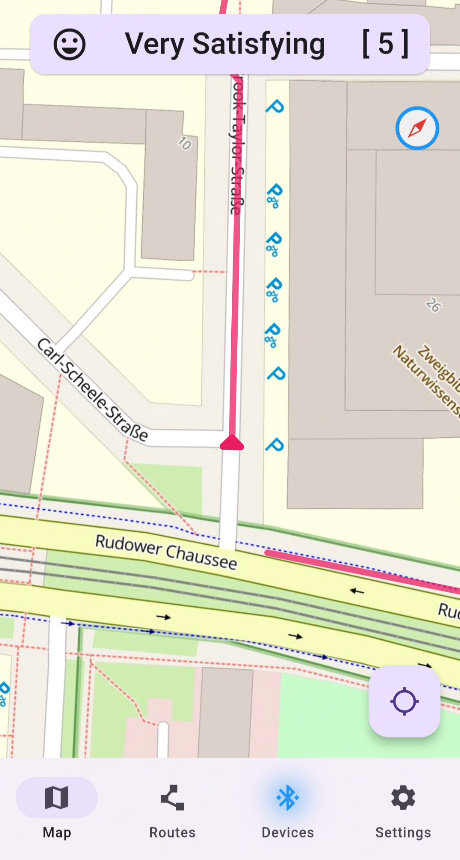
\includegraphics[width=.8666\linewidth]{images/app_map_screen.jpg}
        \caption{\mapscreen}
        \label{subfig:app_map_screen}
    \end{subfigure}%
    \begin{subfigure}{.25\textwidth}
        \centering
        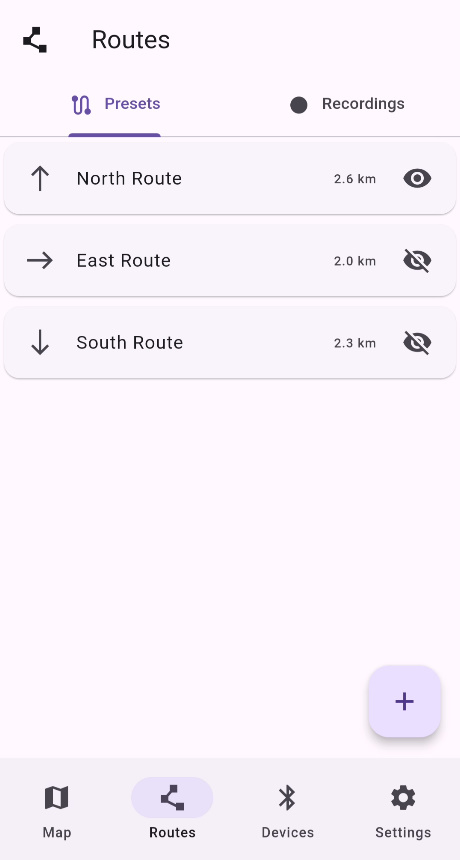
\includegraphics[width=.8666\linewidth]{images/app_routes_screen.jpg}
        \caption{\routesscreen}
        \label{subfig:app_routes_screen}
    \end{subfigure}%
    \begin{subfigure}{.25\textwidth}
        \centering
        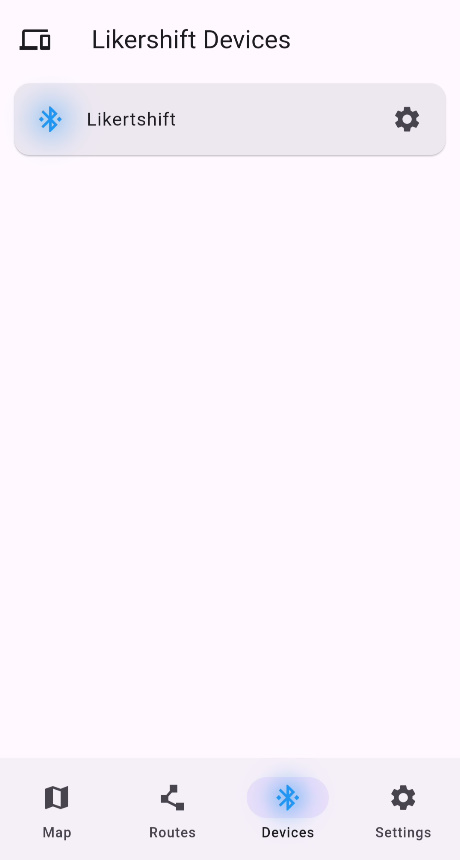
\includegraphics[width=.8666\linewidth]{images/app_devices_screen.jpg}
        \caption{\devicesscreen}
        \label{subfig:app_devices_screen}
    \end{subfigure}%
    \begin{subfigure}{.25\textwidth}
        \centering
        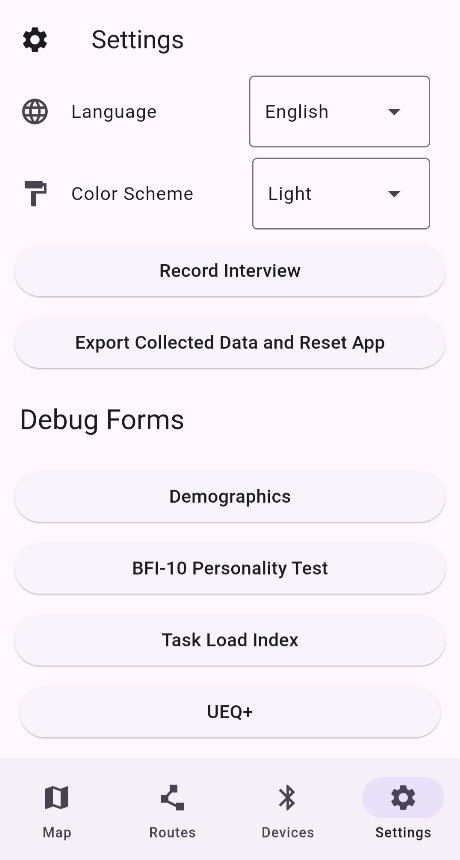
\includegraphics[width=.8666\linewidth]{images/app_settings_screen.jpg}
        \caption{\settingsscreen}
        \label{subfig:app_settings_screen}
    \end{subfigure}
    \caption{An overview of the four main app pages}
\end{figure}

\subsubsection*{Map Screen}

The \mapscreen displays the users current location and surroundings on a 2D map (see \autoref{subfig:app_map_screen}).
It can be moved and rotated using standard touch gestures.
The user can press the bottom-right toggle to make the map automatically follow the current location and long-press the compass to lock the rotation to the current movement direction.
If the user starts a recording, the \mapscreen will also display the travelled route, as well as the preset route, if one was selected.
Additionally, if a \likertshift device is connected, the \mapscreen will also display the devices' currently selected numeric rating and a description of its meaning.
Routes from the \routesscreen can also be previewed on the \mapscreen.

\subsubsection*{Routes Screen and Route Recording}

The \routesscreen is divided into two tabs, showing the available route presets and past recordings respectively (see \autoref{subfig:app_routes_screen}).
Route presets can be previewed using the “Eye” buttons and new recordings can be started using the \raisebox{0.1em}{\textbf{+}} button.

When starting a new recording the user has to select a recording method and optionally a route preset.
Then, whenever the app receives a location update (every $\sim1$--$\SI{5}{s}$), a new data point will be added to the recording, containing the new location, the time elapsed since starting the recording and the current rating value by the active \likertshift device, if available.
This data is then immediately written to a new line in a \texttt{CSV} file, to prevent data loss in case of app crashes or battery run out.
A recording can be stopped at any time by pressing the “Stop Recording” button that will appear above the main navigation bar.
Once a recording is finished, the user can be presented with various forms and surveys (see \autoref{subfig:app_tlx_survey} for an example we used in our field-study).

\subsubsection*{Devices Screen}

The \devicesscreen allows discovering of and connecting to nearby \likertshift devices (see \autoref{subfig:app_devices_screen}).
It displays a list of currently advertising and already known devices.
A new connection can be established by selecting one of the devices from the list.
Only one device can be connected to at any time.
If a connection gets established successfully, its Bluetooth icon lights up, signaling that its currently connected.
During connection, the \likertshift device is queried for its currently selected rating value every \SI{500}{ms} (this update rate can be easily adjusted).
Invalid ratings (see \autoref{subsec:firmware}) are ignored, so the previous rating is kept.

\subsubsection*{Settings Screen}

The apps' language and color theme can be adjusted in the \settingsscreen (see \autoref{subfig:app_settings_screen}).
It has been fully translated to English and German for use in our field-study.
Additionally, it allows navigating to the \textsf{Interview Recording Screen}, which offers a simple interface to start, pause and stop recording an audio interview (see \autoref{subfig:app_interview_recorder}).
Recorded audio interviews will also be saved locally as losslessly encoded \texttt{FLAC} files.
Finally, the \settingsscreen offers a button to “Export collected Data and Reset the App” which will bundle all recorded data into a single \texttt{ZIP} file and store it locally, under a randomly generated participant ID.
Said ID will then be reported back to the user, and the app will be reset (see \autoref{subfig:app_data_export}).

\begin{figure}[!htb]
    \centering
    \begin{subfigure}{.25\textwidth}
        \centering
        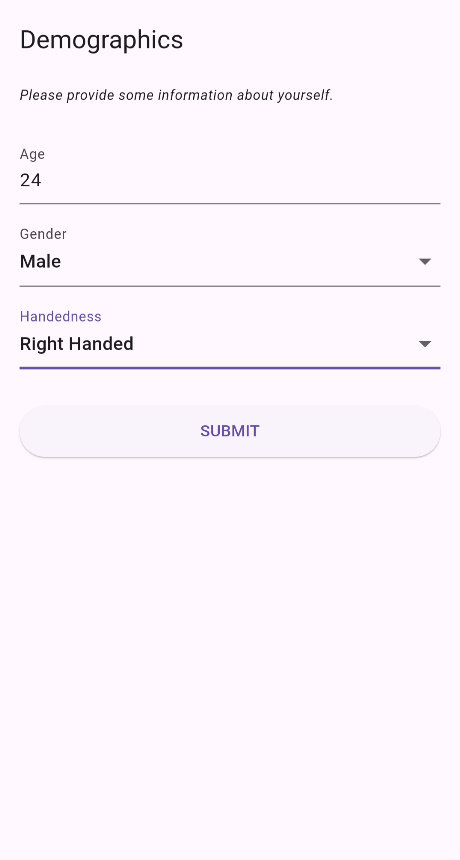
\includegraphics[width=.8666\linewidth]{images/app_demographics_form.jpg}
        \caption{Demographics form}
        \label{subfig:app_demographics_form}
    \end{subfigure}%
    \begin{subfigure}{.25\textwidth}
        \centering
        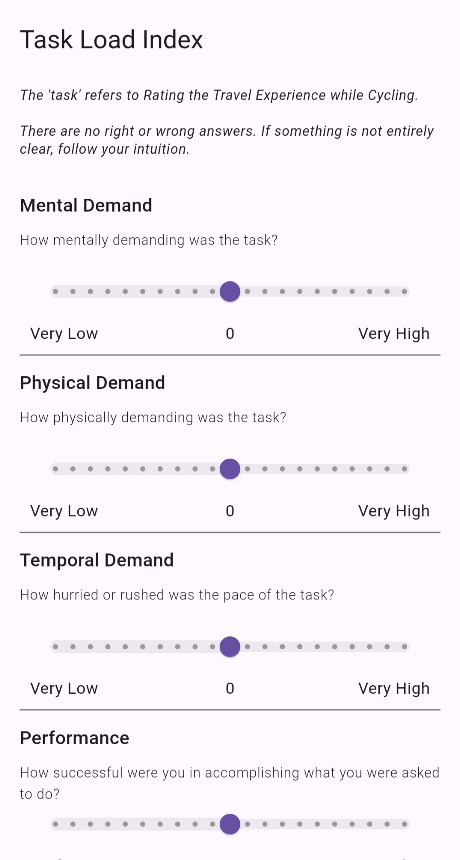
\includegraphics[width=.8666\linewidth]{images/app_tlx_survey.jpg}
        \caption{TLX survey}
        \label{subfig:app_tlx_survey}
    \end{subfigure}%
    \begin{subfigure}{.25\textwidth}
        \centering
        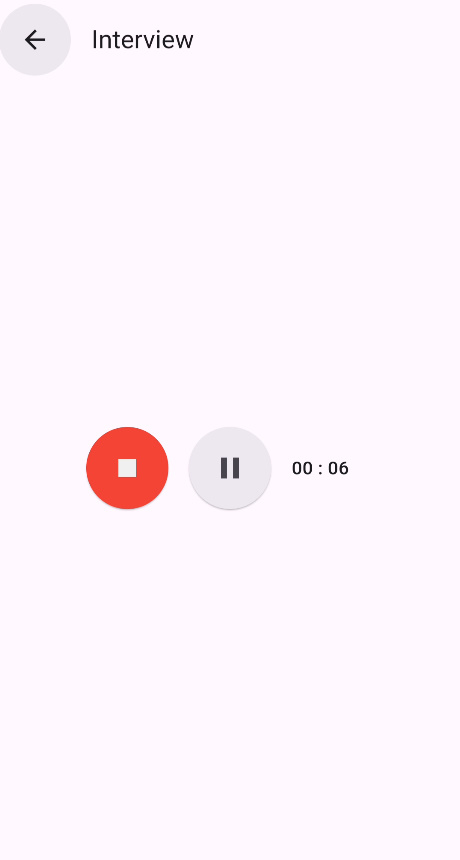
\includegraphics[width=.8666\linewidth]{images/app_interview_recorder.jpg}
        \caption{Interview recorder}
        \label{subfig:app_interview_recorder}
    \end{subfigure}%
    \begin{subfigure}{.25\textwidth}
        \centering
        
\includegraphics[width=.8666\linewidth]{images/app_reset_screen.jpg}
        \caption{Data export}
        \label{subfig:app_data_export}
    \end{subfigure}
    \caption{Contextual screens}
\end{figure}

\noindent
The app is written using the Flutter\footnoteurl{https://flutter.dev/} framework and Dart\footnoteurl{https://dart.dev/} programming language.
While we only tested and used our app on Android devices, the multi-platform nature of Flutter should also allow it to run on iOS powered devices with minimal modifications.

\newpage\section{Study Design}\label{sec:study_design}

We decided to evaluate our prototype in a semi-naturalistic field-study, comparing it against similar methods, capable of recording \CSE for individual segments of a larger route.
This section describes how we went about designing this study.

\subsection{Recording Methods}\label{subsec:recording_methods}

Our method using the \likertshift device works by recording its currently selected value, whenever we receive a new GPS location.
Thus, a selected value remains valid until the users selects a new one, and we receive their next GPS location, so a new rating gets recorded whenever they notice a change in their subjective experience and remains valid, onwards from that point in time, until they adjust the rating again.
This allows users to choose a rating frequency they consider appropriate by themselves.

We selected two methods from our survey of the related work we regard as suitable to compare against our method and adjusted them, to allow for a fair comparison.
The first one, referred to as \audiorecording from now on, is taken from the work of \citetext{evaluation_models_for_cyclists_perception}{Yamanaka et al.}, who captured audio data while cycling and required participants to rate pre-defined route-segments using multiple measures on scales from 1 to 5.
We adjusted it to only used one measure and also let participants perform ratings on arbitrary route segments, in contrast to pre-defined ones.
The second method, referred to as \mapping is the one proposed by \citetext{using_mental_mapping}{Manton et al.}, who let participants color code segments of a previously driven route, based on their risk assessment.
In our study, we provided participants with a printed map, picturing the route they drove and let them divide it into multiple segments themselves, assigning a numerical rating to each segment, instead of color coding it.

\subsubsection*{Choosing a Measure}

We had to take great care to select a suitable measure, so we could compare the data collected by different participants and the different methods against each other.
This is inherently difficult, as cyclists' subjective experiences are arguably very subjective and will therefore vary drastically from participant to participant.

As mentioned in the introduction to \autoref{sec:related_work}, most works rely on risk/safety and stress/comfort measures to quantify \CSE.
The advantage of using risk/safety would be its independence from many external factors and high dependence on the chosen route.
Constructing a route with highly varying risk factors would be comparatively easy, but deliberately placing participants in high-risk environments would be extremely unethical, which led us to quickly dismiss that approach.
Letting participants rate their comfort level or travel satisfaction comes with its own set of challenges though.
Overall comfort level depends on a lot of factors, such as participants initial mood, their experience in riding a bicycle, but also external factors such as weather, traffic, or surrounding scenery of the route.
To be able to properly compare our recorded datasets against each other, we needed to find a way to eliminate as many of these factors as possible.

As findings by \citetext{thinking_aloud_on_the_road}{McIlroy et al.} revealed the high impact of road surface quality on cyclists overall comfort and satisfaction with their travel, we decided to limit our measure to this, using the metric of “Travel satisfaction, based on the road” as the \CSE measure that participants have to use to rate segments of the route.
We carefully explained this metric to each participant before conducting the study, instructing them on what should (road condition, road type, available space, slope of the road, etc.) and should not (general mood, current traffic situation, route scenery, etc.) affect their ratings.
Ratings were to be performed on a Likert scale from 1 to 5, denoting high dissatisfaction and high satisfaction, respectively.
This measure should exert a similar mental demand on participants, as they still need to feel out their comfort level, while increasing data quality, allowing us to perform quantitative comparisons of the different methods used.
\subsection{Route Selection}

If each participant was to evaluate all three methods after each other on the same route, we would expect to see an increase in accuracy for subsequent route traversals, as by that point the route is already known.
Thus, we constructed three different routes and balanced route orders, method orders as well as the number of routes per method in our study.
We chose each route to take $\sim\SI{10}{min}$ to complete for an average cyclist and ensured it contained a multitude of different road types and crossings.
As we wanted to conduct the study in a single session per participant, at our university campus, we were limited by the available traffic infrastructure in the immediate vicinity and also had to put all start and endpoints in the approximate same location.

\begin{table}[!htb]
    \footnotesize
    \centering
    \begin{tabular}{c|c|ccccc|c}
        \multirow{2}{*}{Name} & \multirow{2}{2.4em}{Total\newline} & \multicolumn{5}{c|}{Road Type} & \multirow{2}{4.7em}{Number of\newline}\\
        \cline{3-7}
        &&&&&&&\\[-1em]
        & Length & Road & Bike Path & Mixed Path & Pedestrian Way & Other & Crossings\\[0.15em]
        \hline
        &&&&&&&\\[-0.8em]
        North & \SI{2589}{m} &  \SI{191}{m} & \SI{480}{m} & \SI{1135}{m} & \SI{359}{m} & \SI{424}{m} & 13\\[0.3em]
        East  & \SI{2007}{m} &  \SI{853}{m} & \SI{465}{m} &  \SI{173}{m} & \SI{181}{m} & \SI{335}{m} & 9\\[0.3em]
        South & \SI{2289}{m} & \SI{1152}{m} & \SI{677}{m} &  \SI{116}{m} &  \SI{47}{m} & \SI{297}{m} & 9\\
    \end{tabular}
    \caption{Overview of the study routes}
    \label{table:routes_overview}
\end{table}

\noindent
\autoref{table:routes_overview} shows the total lengths of the routes, as well as an overview of the different road types and number of crossings per route.
Each route is named according to the direction it starts towards.
The study was conducted at the Campus Adlershof\footnoteurl{https://www.hu-berlin.de/en/about/campus/adlershof} of the Humboldt University of Berlin, located in a mixed-use area outside the city center.
Notably, the roads participants had to drive on were mostly side-roads with very little traffic and therefore received a more positive rating than one might expect.
We also opted to use existing cycling infrastructure wherever possible, only evading to drive on the road when no such infrastructure was available.
Furthermore, mixed-paths refer to areas mainly intended to be used by pedestrians that are spacious enough to allow for cycling at low speeds.

\begin{figure}[!htb]
    \centering
    \begin{minipage}{.5\textwidth}
        \centering
        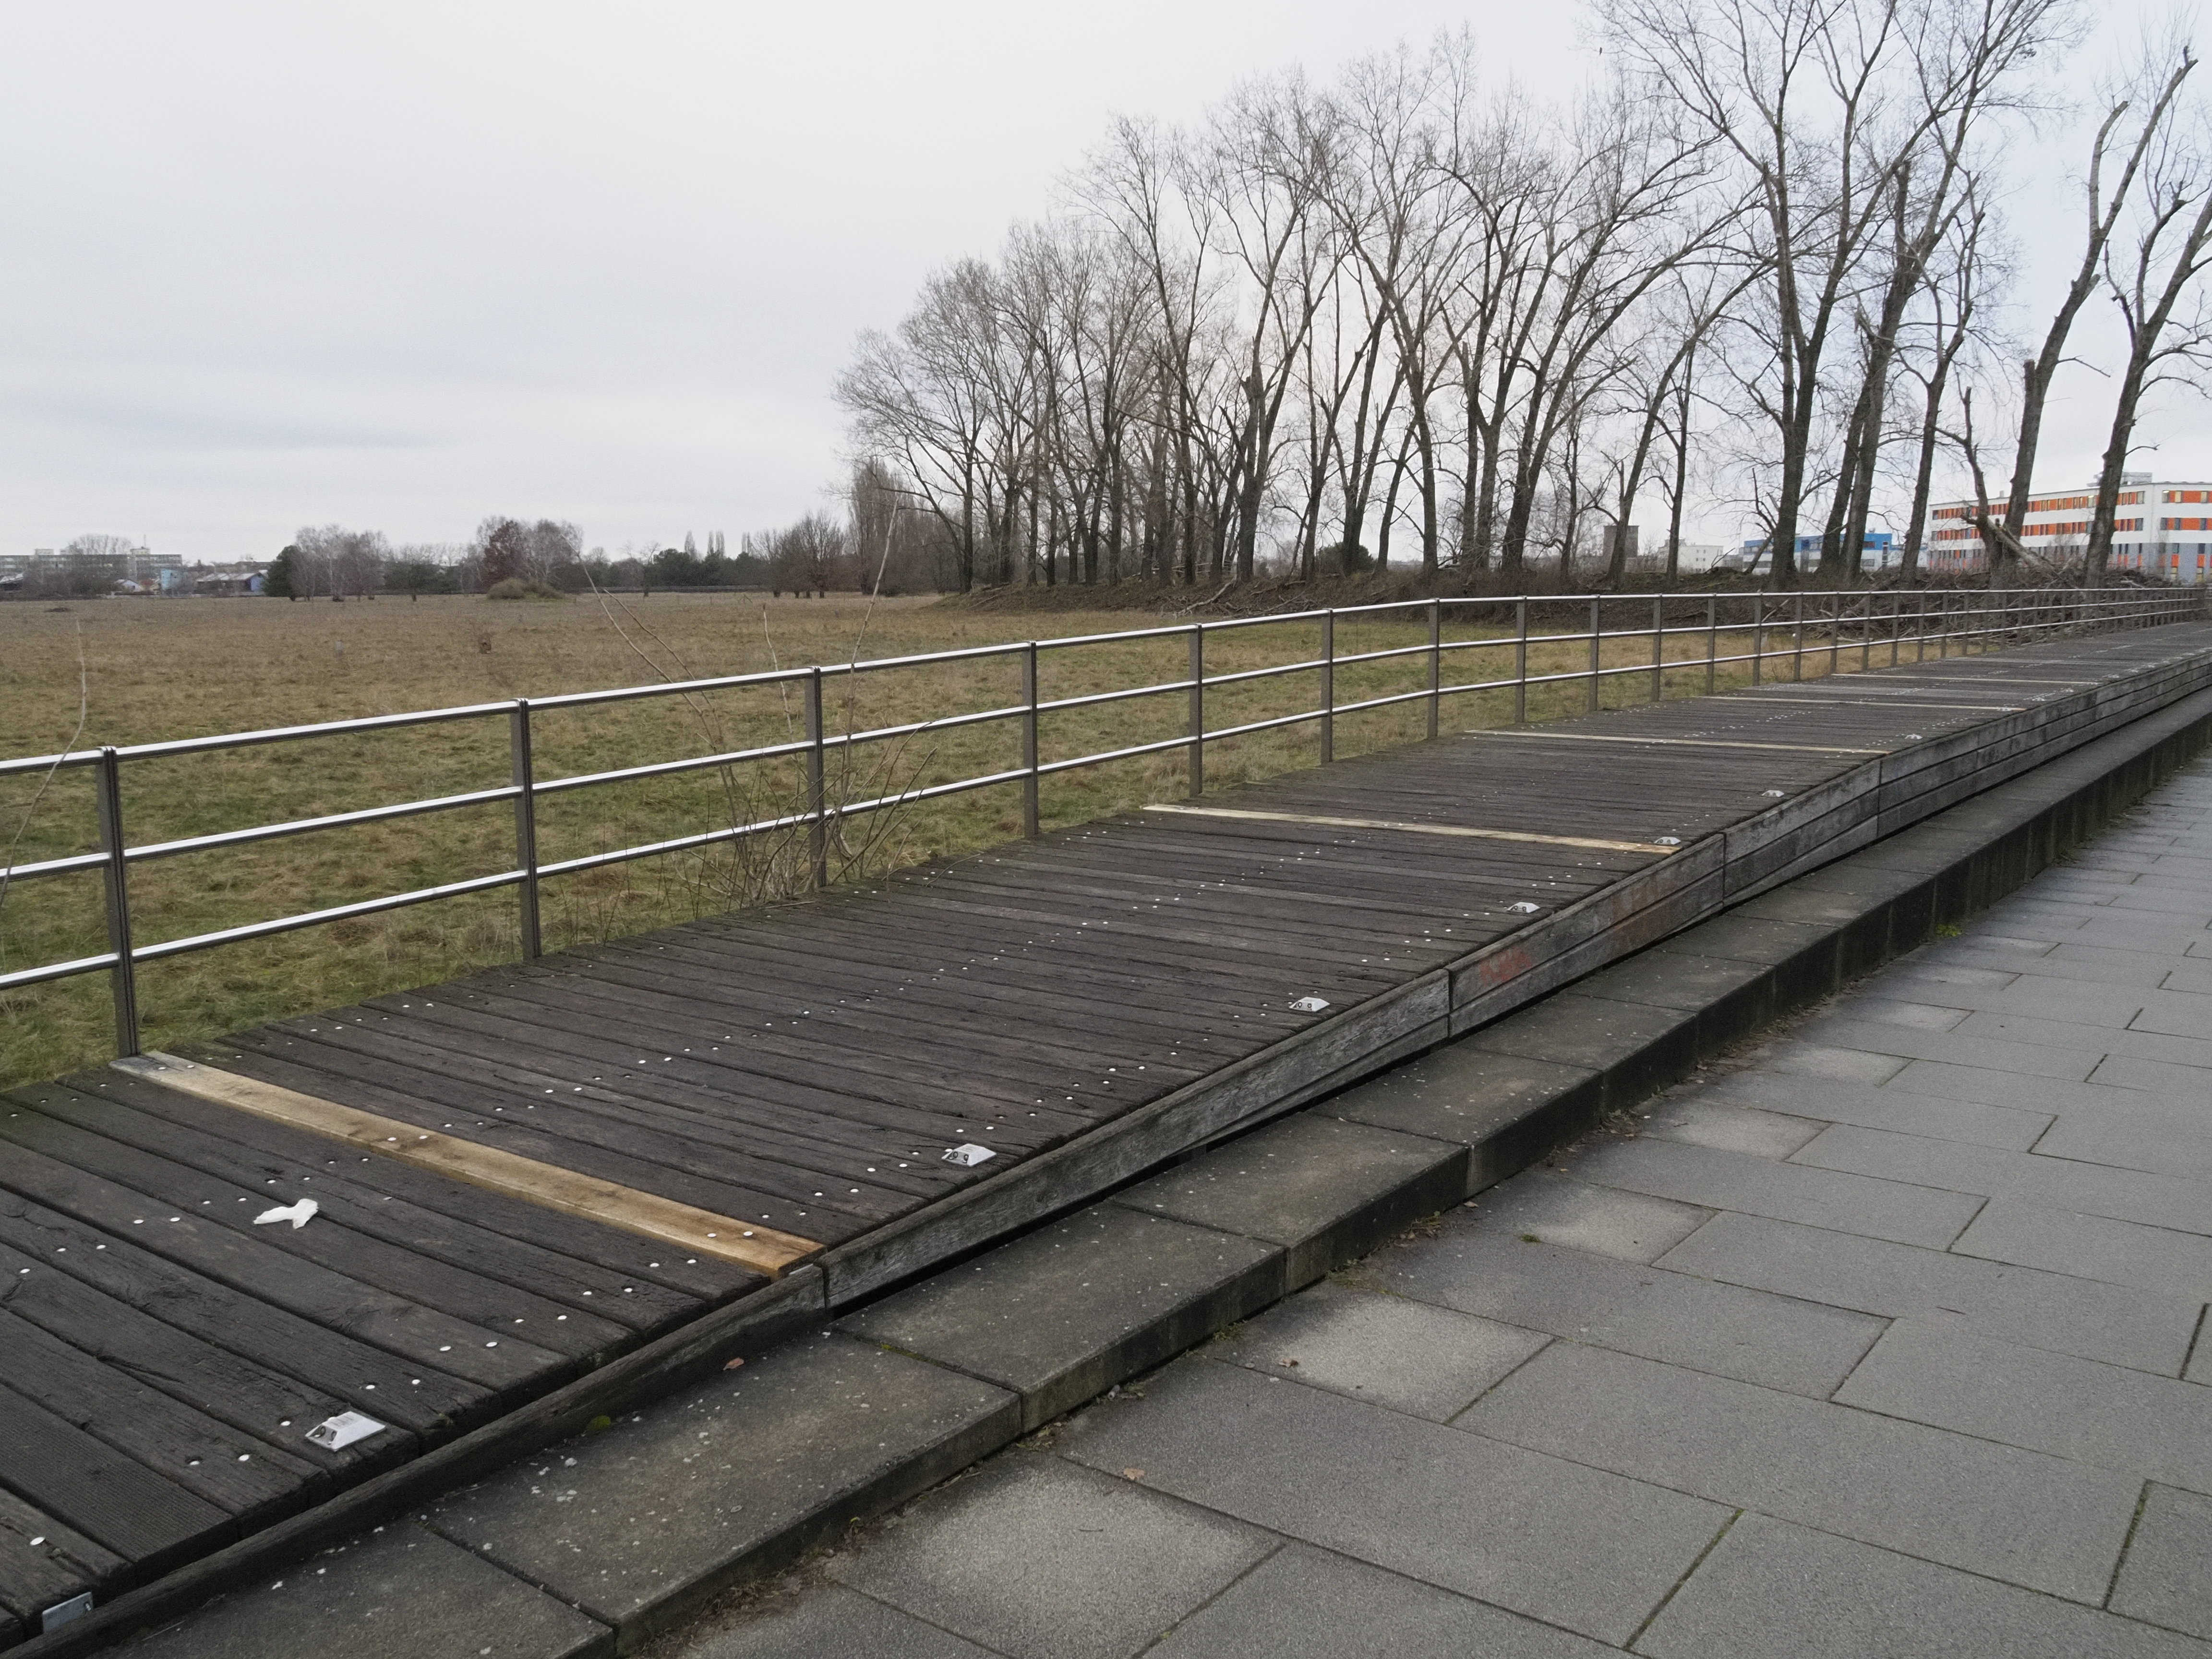
\includegraphics[width=.9333\linewidth]{images/wood_planks_path.jpg}
        \caption{Elevated path (wood planks)}
        \label{fig:wood_planks}
    \end{minipage}%
    \begin{minipage}{.5\textwidth}
        \centering
        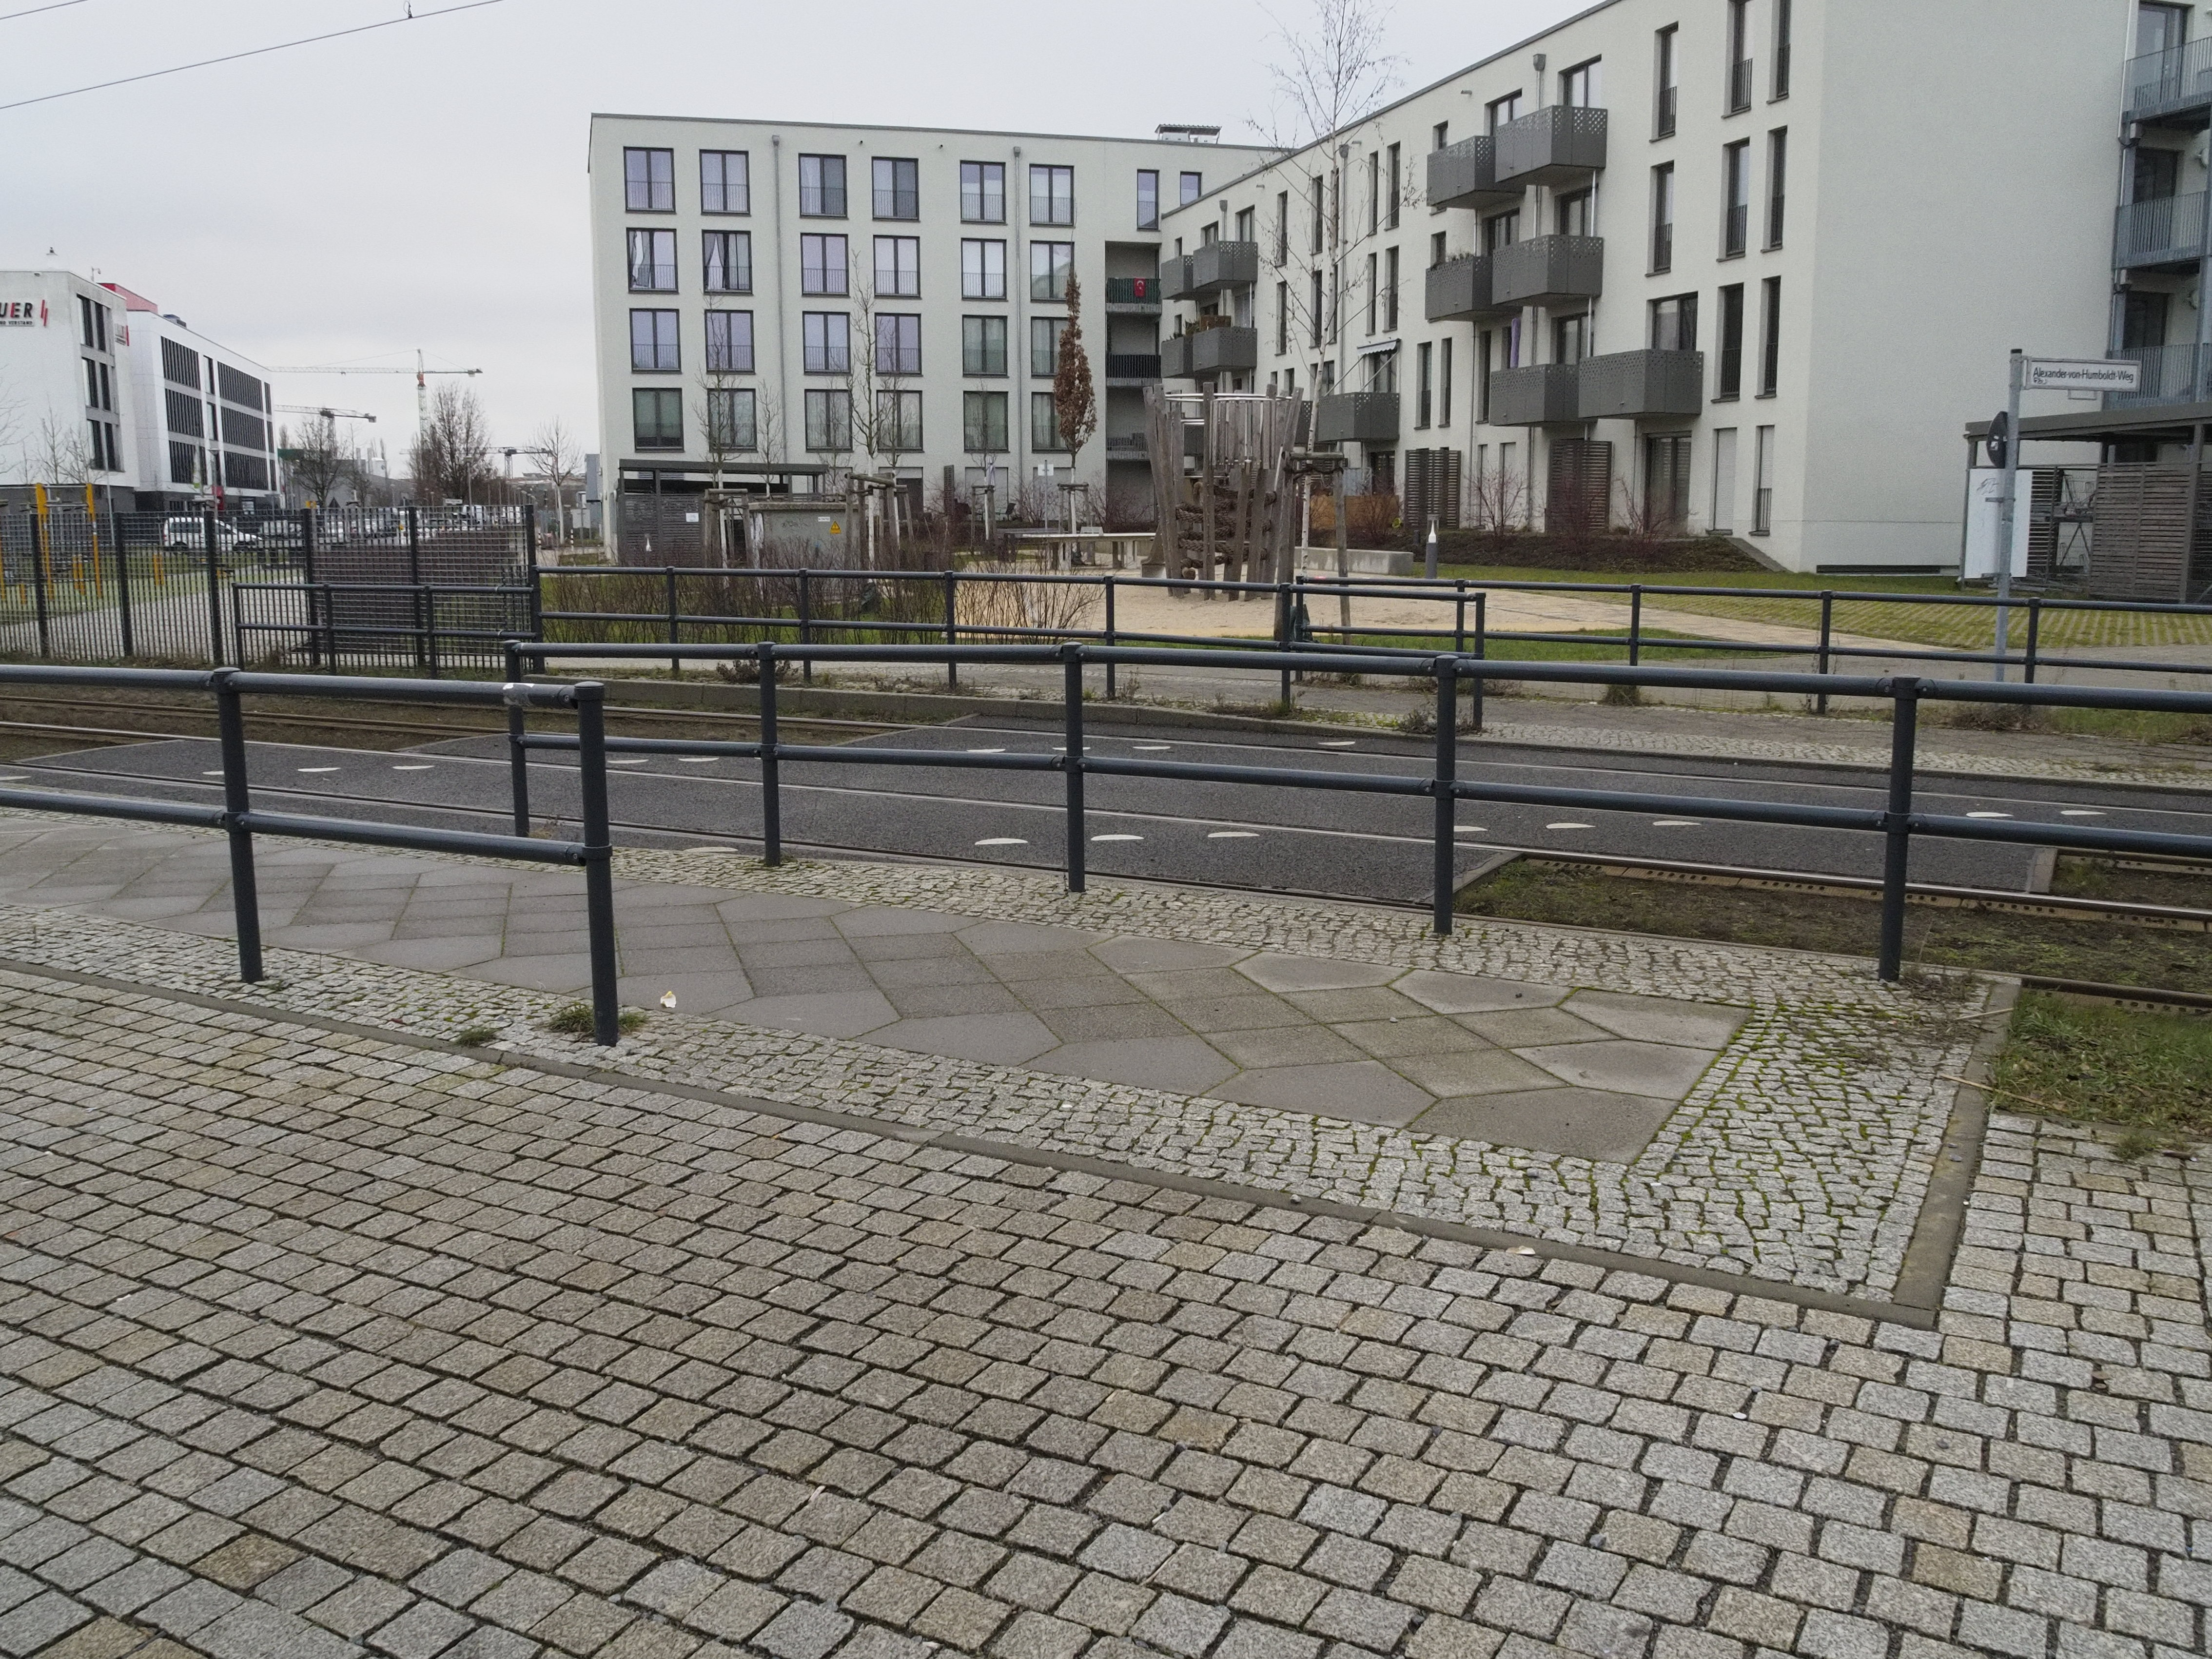
\includegraphics[width=.9333\linewidth]{images/tram_crossing.jpg}
        \caption{Tram crossing}
        \label{fig:tram_crossing}
    \end{minipage}
\end{figure}

\bigbreak\noindent
We also chose each route to contain at least one section that particularly stands out from the rest of the route.
For the “North” route this was an elevated wooden path (\autoref{fig:wood_planks}), as well as an awkward tram crossing (\autoref{fig:tram_crossing}).
The “East” route contained the objectively worst terrain of our study, a very rugged field participants had to traverse (\autoref{fig:field_east}).
The “South” route also featured an “off-road” section, traversing a lawn next to a building, this one was noticeably more flat though (\autoref{fig:field_south}).
The “East” and “South” routes also both featured different sections blocked by the same construction site (\autoref{fig:construction_site}), where participants had to result to driving on pedestrian ways.

\begin{figure}[!htb]
    \centering
    \begin{minipage}{.3333\textwidth}
        \centering
        \includegraphics[width=.9\linewidth]{images/field_east_route.jpg}
        \caption{Rugged field}
        \label{fig:field_east}
    \end{minipage}%
    \begin{minipage}{.3333\textwidth}
        \centering
        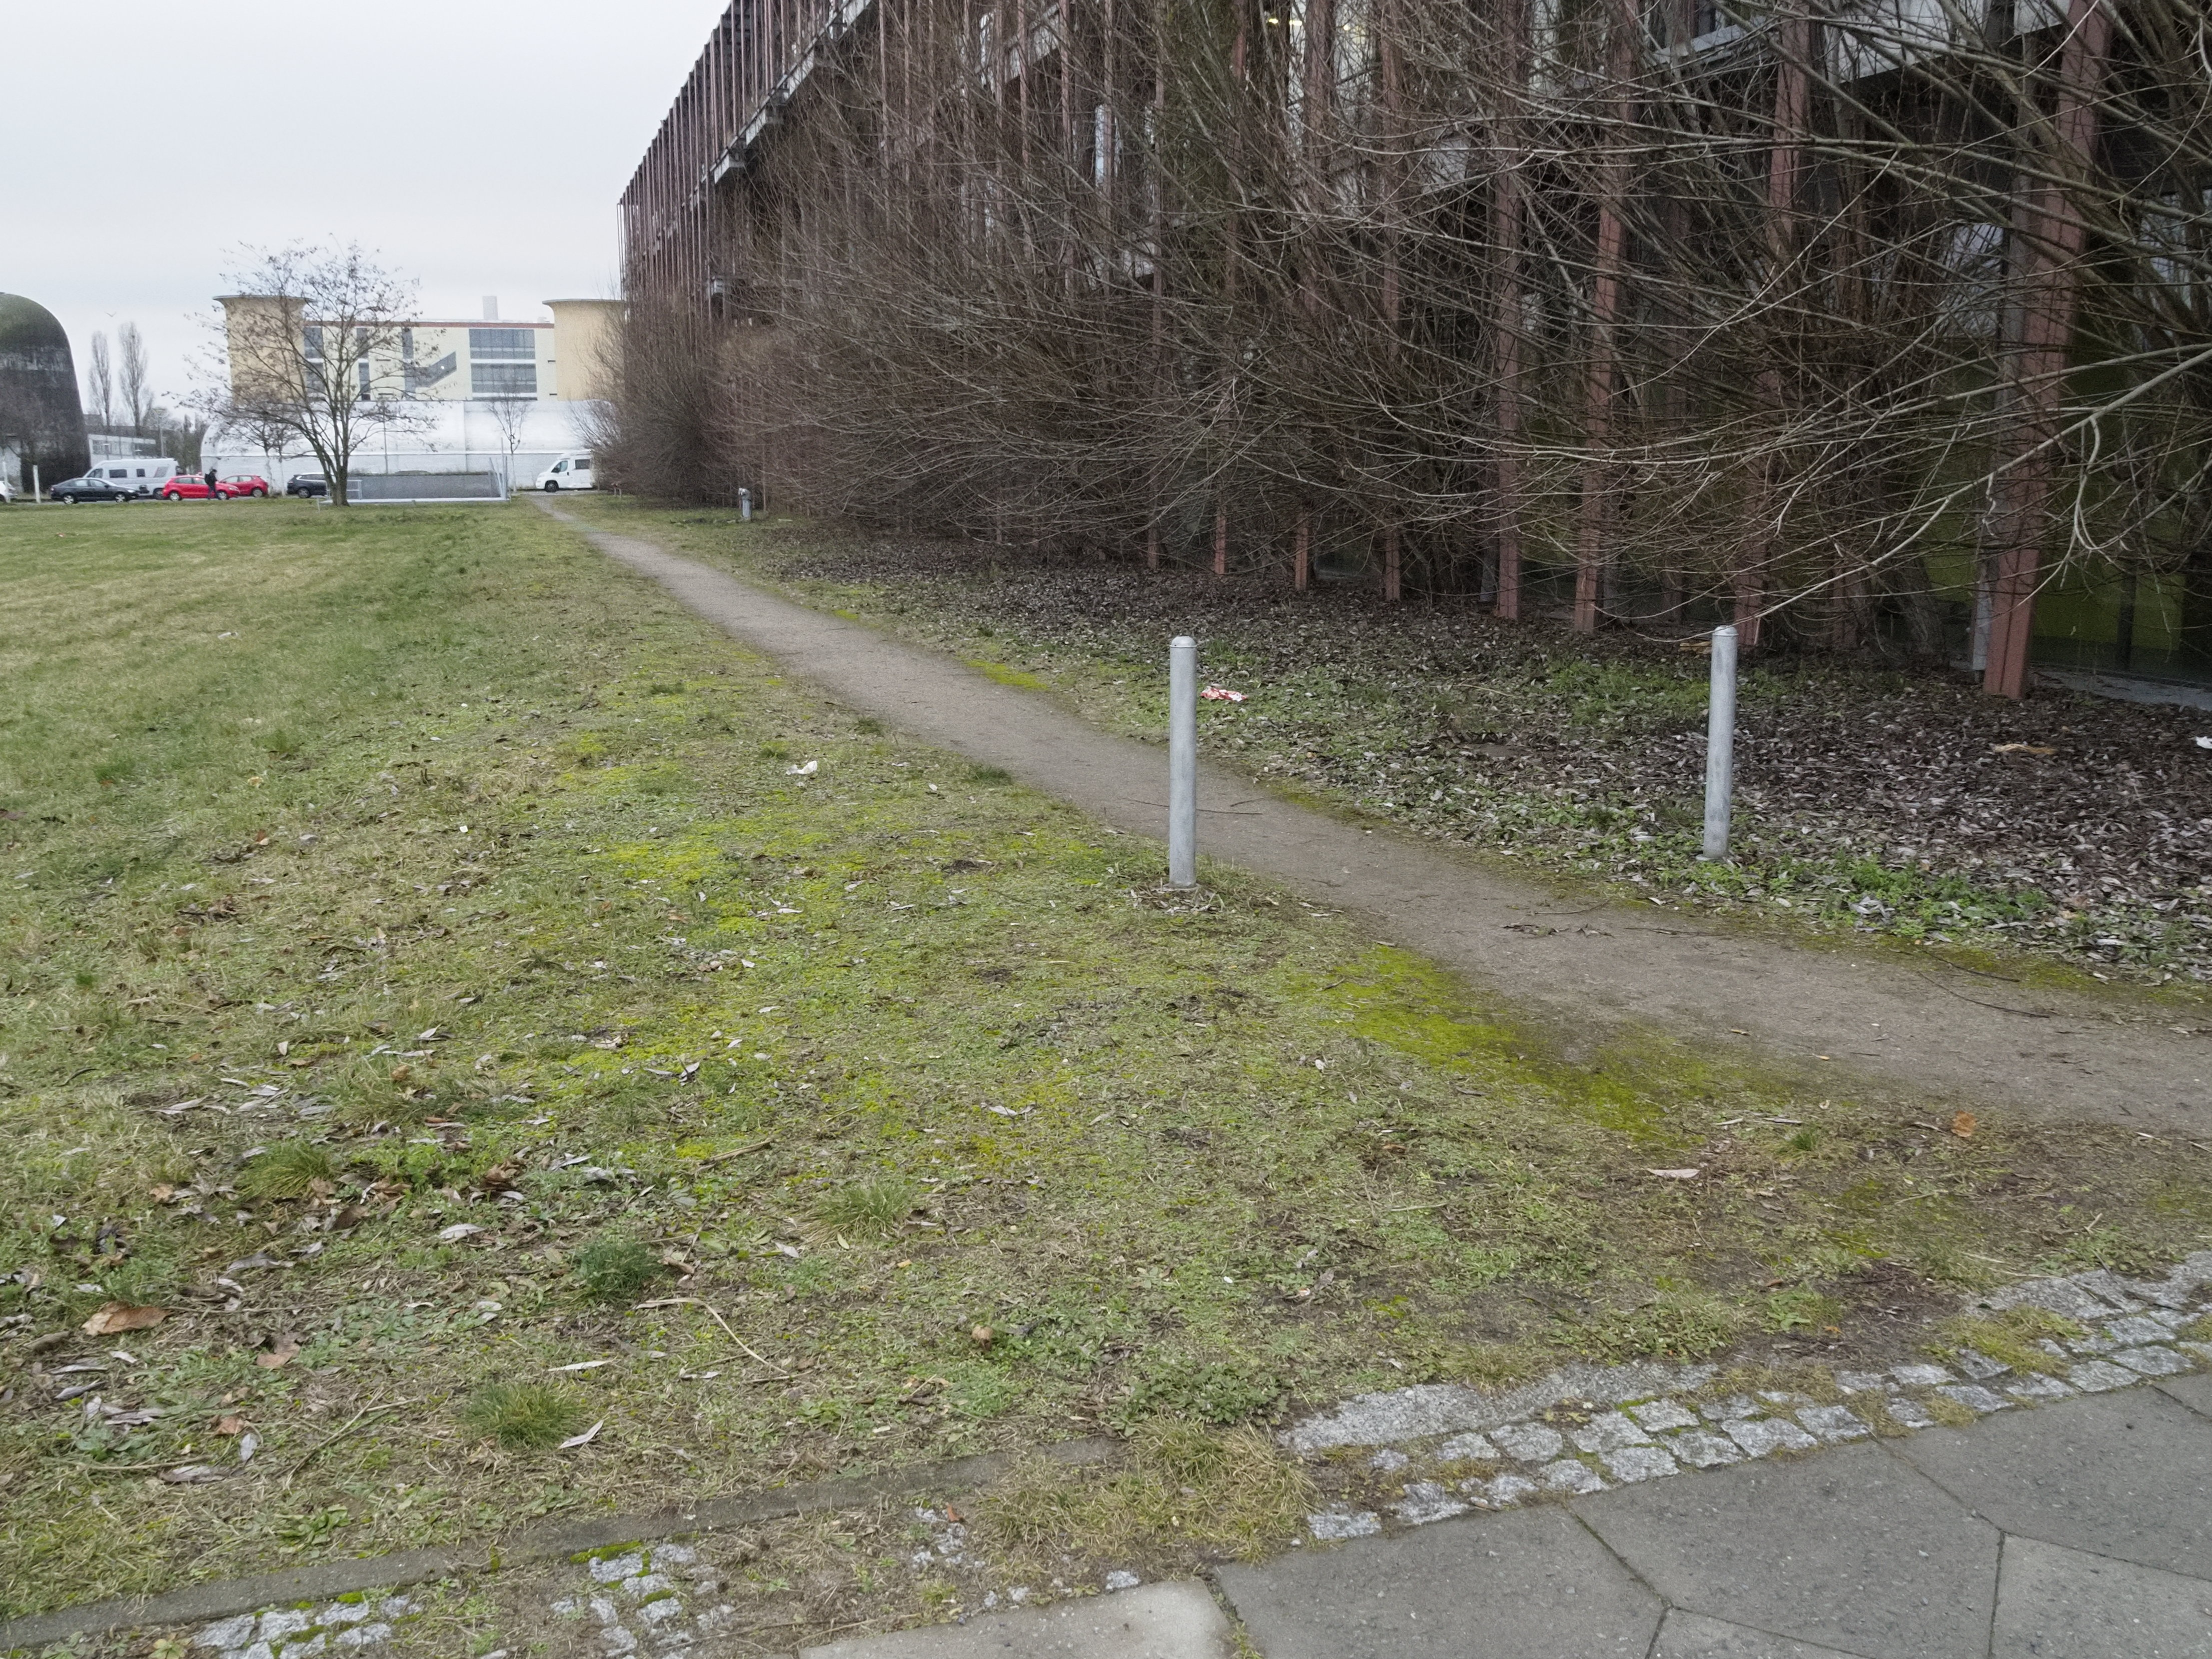
\includegraphics[width=.9\linewidth]{images/field_south_route.jpg}
        \caption{Flat lawn}
        \label{fig:field_south}
    \end{minipage}%
    \begin{minipage}{.3333\textwidth}
        \centering
        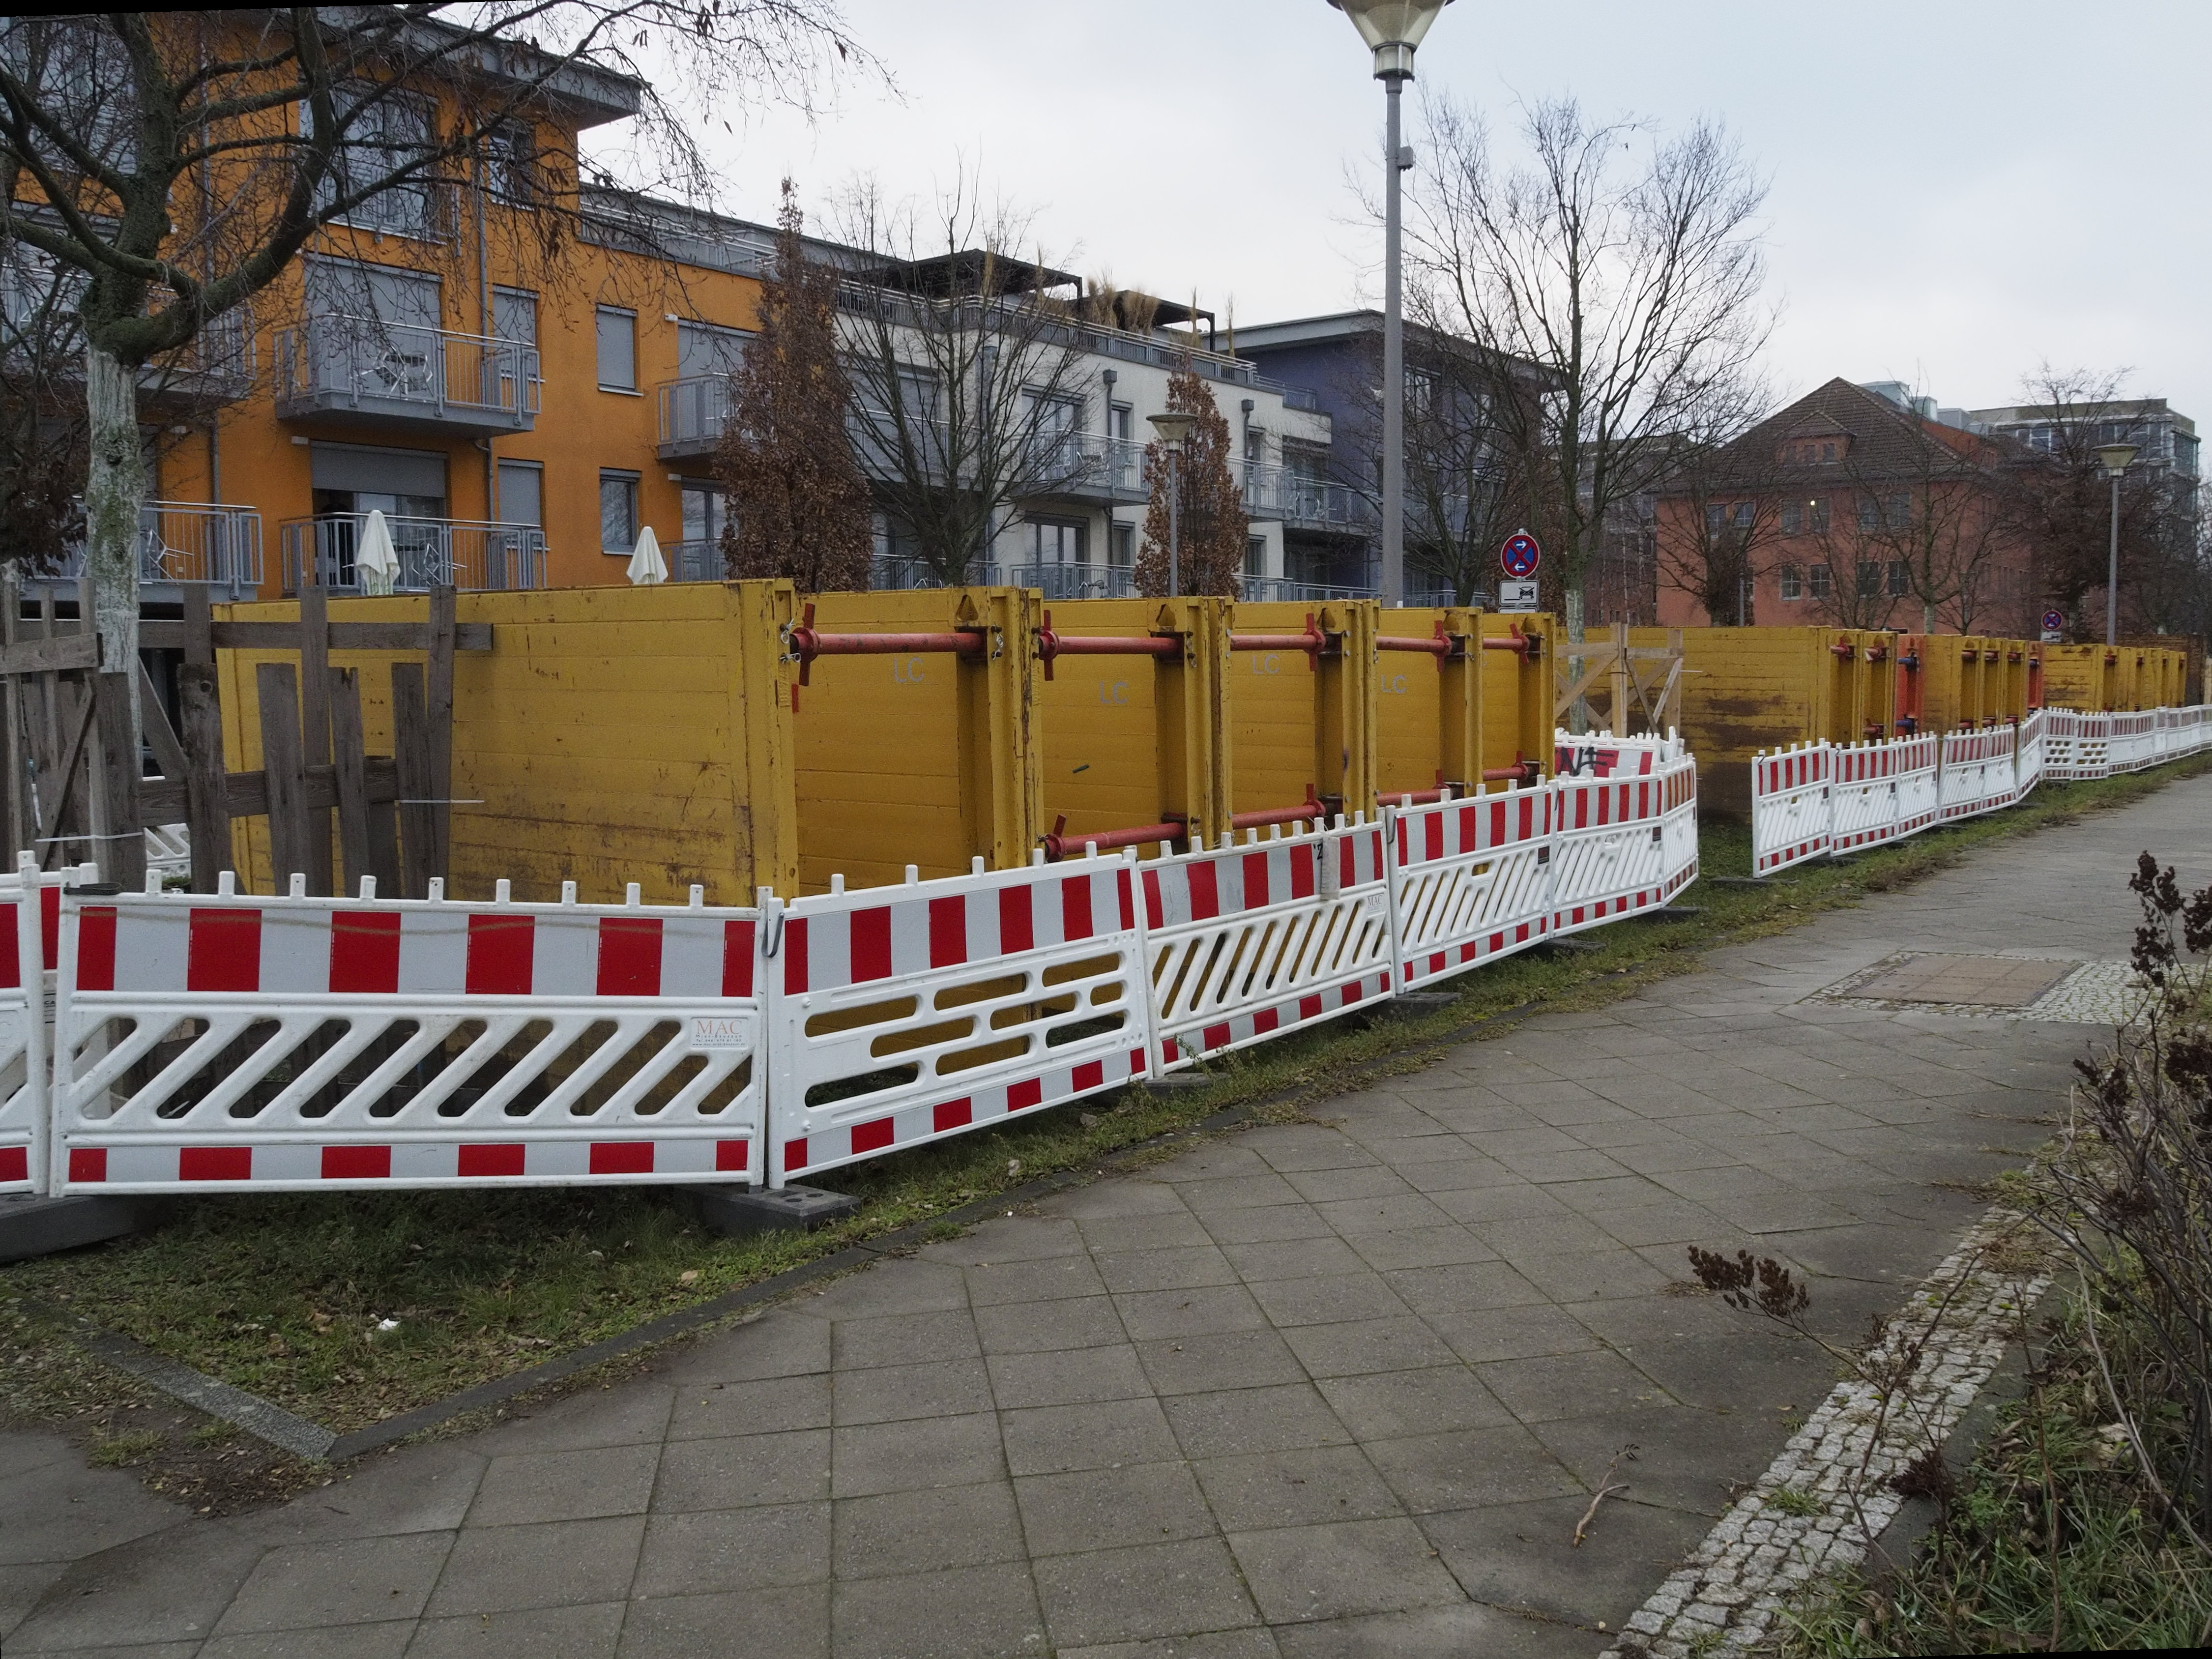
\includegraphics[width=.9\linewidth]{images/construction_site.jpg}
        \caption{Construction site}
        \label{fig:construction_site}
    \end{minipage}
\end{figure}

\subsection{Data Collection}\label{subsec:data_collection}

All data was collected using the \likertshift app acting as a frontend for our prototype, as described in \autoref{subsec:frontend_design} and the \audiorecording and \mapping methods were added to it.
\audiorecording is implemented by using the smartphones internal microphone to record an audio track while cycling.
The recorded audio will then be added to the recording data as a lossless \texttt{FLAC} file.
For the \mapping method, we only recorded location and time information in the app.
The actual ratings were performed retrospectively on a piece of paper.
After resetting the app at the end of each study participation, we simply wrote down the participants ID on said piece of paper, to be able to match it with the recorded data later on.
This is described in more detail in \autoref{subsec:preprocessing}.

\subsubsection{Questionnaires}

In addition to this quantitative data, we also used two questionnaires, the \citetext{nasa_tlx}{NASA TLX} and the \citetext{ueq+}{UEQ+} (a modular extension of the commonly used \citetext{ueq}{UEQ}) to obtain qualitative data, regarding differences between the recording methods used.
Participants were asked to fill in these questionnaires right after they finished rating a route with each method.
We made sure participants understood that both questionnaires only concerned the respective method used to rate their subjective experience during cycling, but not the act of cycling itself.
For the \citetextnoref{ueq+}{UEQ+}, we selected the \textit{Attractiveness}, \textit{Efficiency}, \textit{Intuitive Use}, \textit{Hardware Security} and \textit{Social Acceptance} scales and slightly adjusted some questions wordings, as the \citetextnoref{ueq+}{UEQ+} is usually used to evaluate the user experience of products, not methods.

\subsubsection{Interview}

We also conducted a short $\sim\SI{10}{min}$ interview with every participant, asking them about their frequency of and reasoning for cycling, a ranking of the three methods used to record their subjective experience, as well as problems that could occur and possible improvements for each of the methods.
Additionally, we asked what kind of bicycles participants used privately and whether our devices would be able to be mounted to them in its current form, to assess the compatibility of our method with different types of bicycles.

\subsection{Procedure}

We started by giving an introduction to the study as well as the methods used and explained the general order of operations and approximate duration.
We also provided participants with an informed consent sheet, outlining the procedure, associated risks, our data protection guidelines and information about compensation, which they had to sign.
They then got introduced to out \likertshift app and had to fill in the initial demographics form.
Next, participants were shown the bicycle used for performing the study (\autoref{fig:study_bike}) and then asked to adjust the saddle height to their liking and to drive along a short test route, to get used to it.
Then, we randomly selected a row from our balancing sheet (containing three method/route combinations, with each method and route only appearing once).
For each of these combinations, we first explained the method used to participants and asked them if they would like to perform another short test drive to simulate using said method.
Once done, participants drove the respective route and after submitting their ratings, also filled in our prepared questionnaires in the \likertshift app.
During the ride, a smartphone was mounted to the bicycle, in between the handlebars (\autoref{fig:smartphone_holder}), running the \likertshift app which displayed the route participants had to follow and recorded the required data.
After all three combinations were completed, we finished by carrying out our interview.

% linewidth_factor = 1 - (1 / (30 * textwidth_factor))
% textwidth_factor ~ 4/7 (adjusted by hand)
\begin{figure}[!htb]
    \centering
    \begin{minipage}{.5675\textwidth}
        \centering
        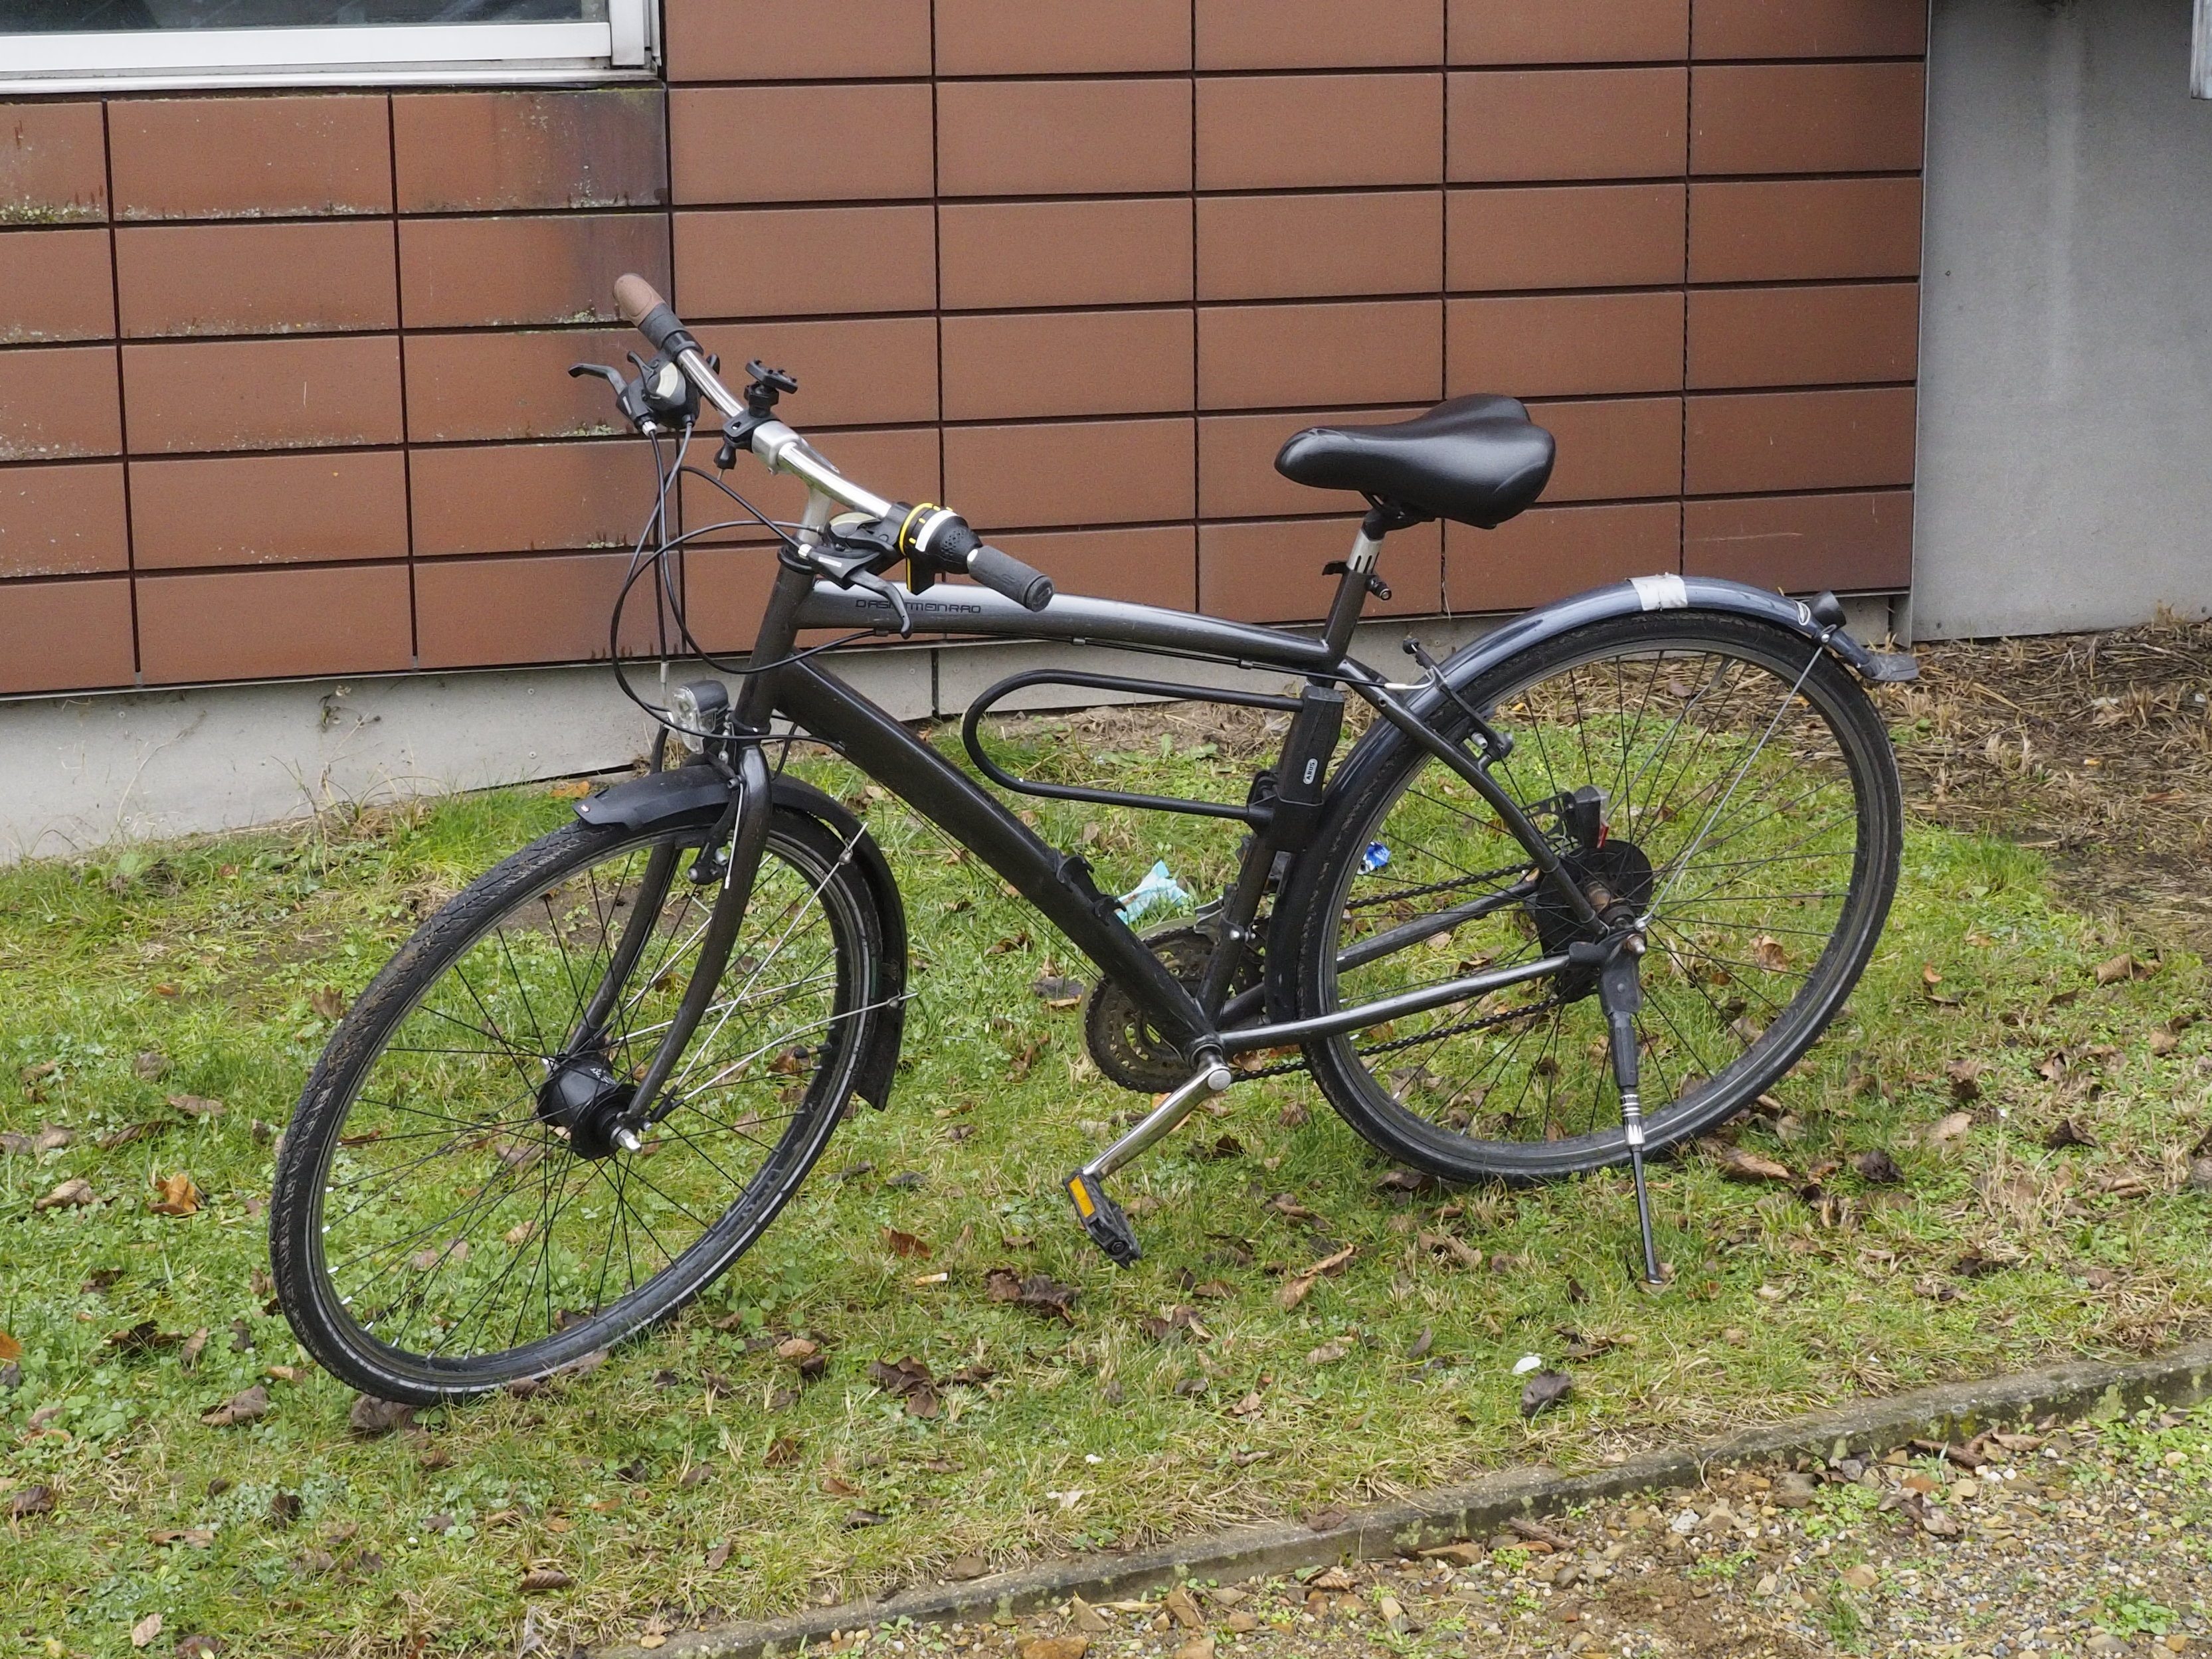
\includegraphics[width=.9413\linewidth]{images/study_bike.jpg}
        \caption{The bicycle used in the field-study}
        \label{fig:study_bike}
    \end{minipage}%
    \begin{minipage}{.4325\textwidth}
        \centering
        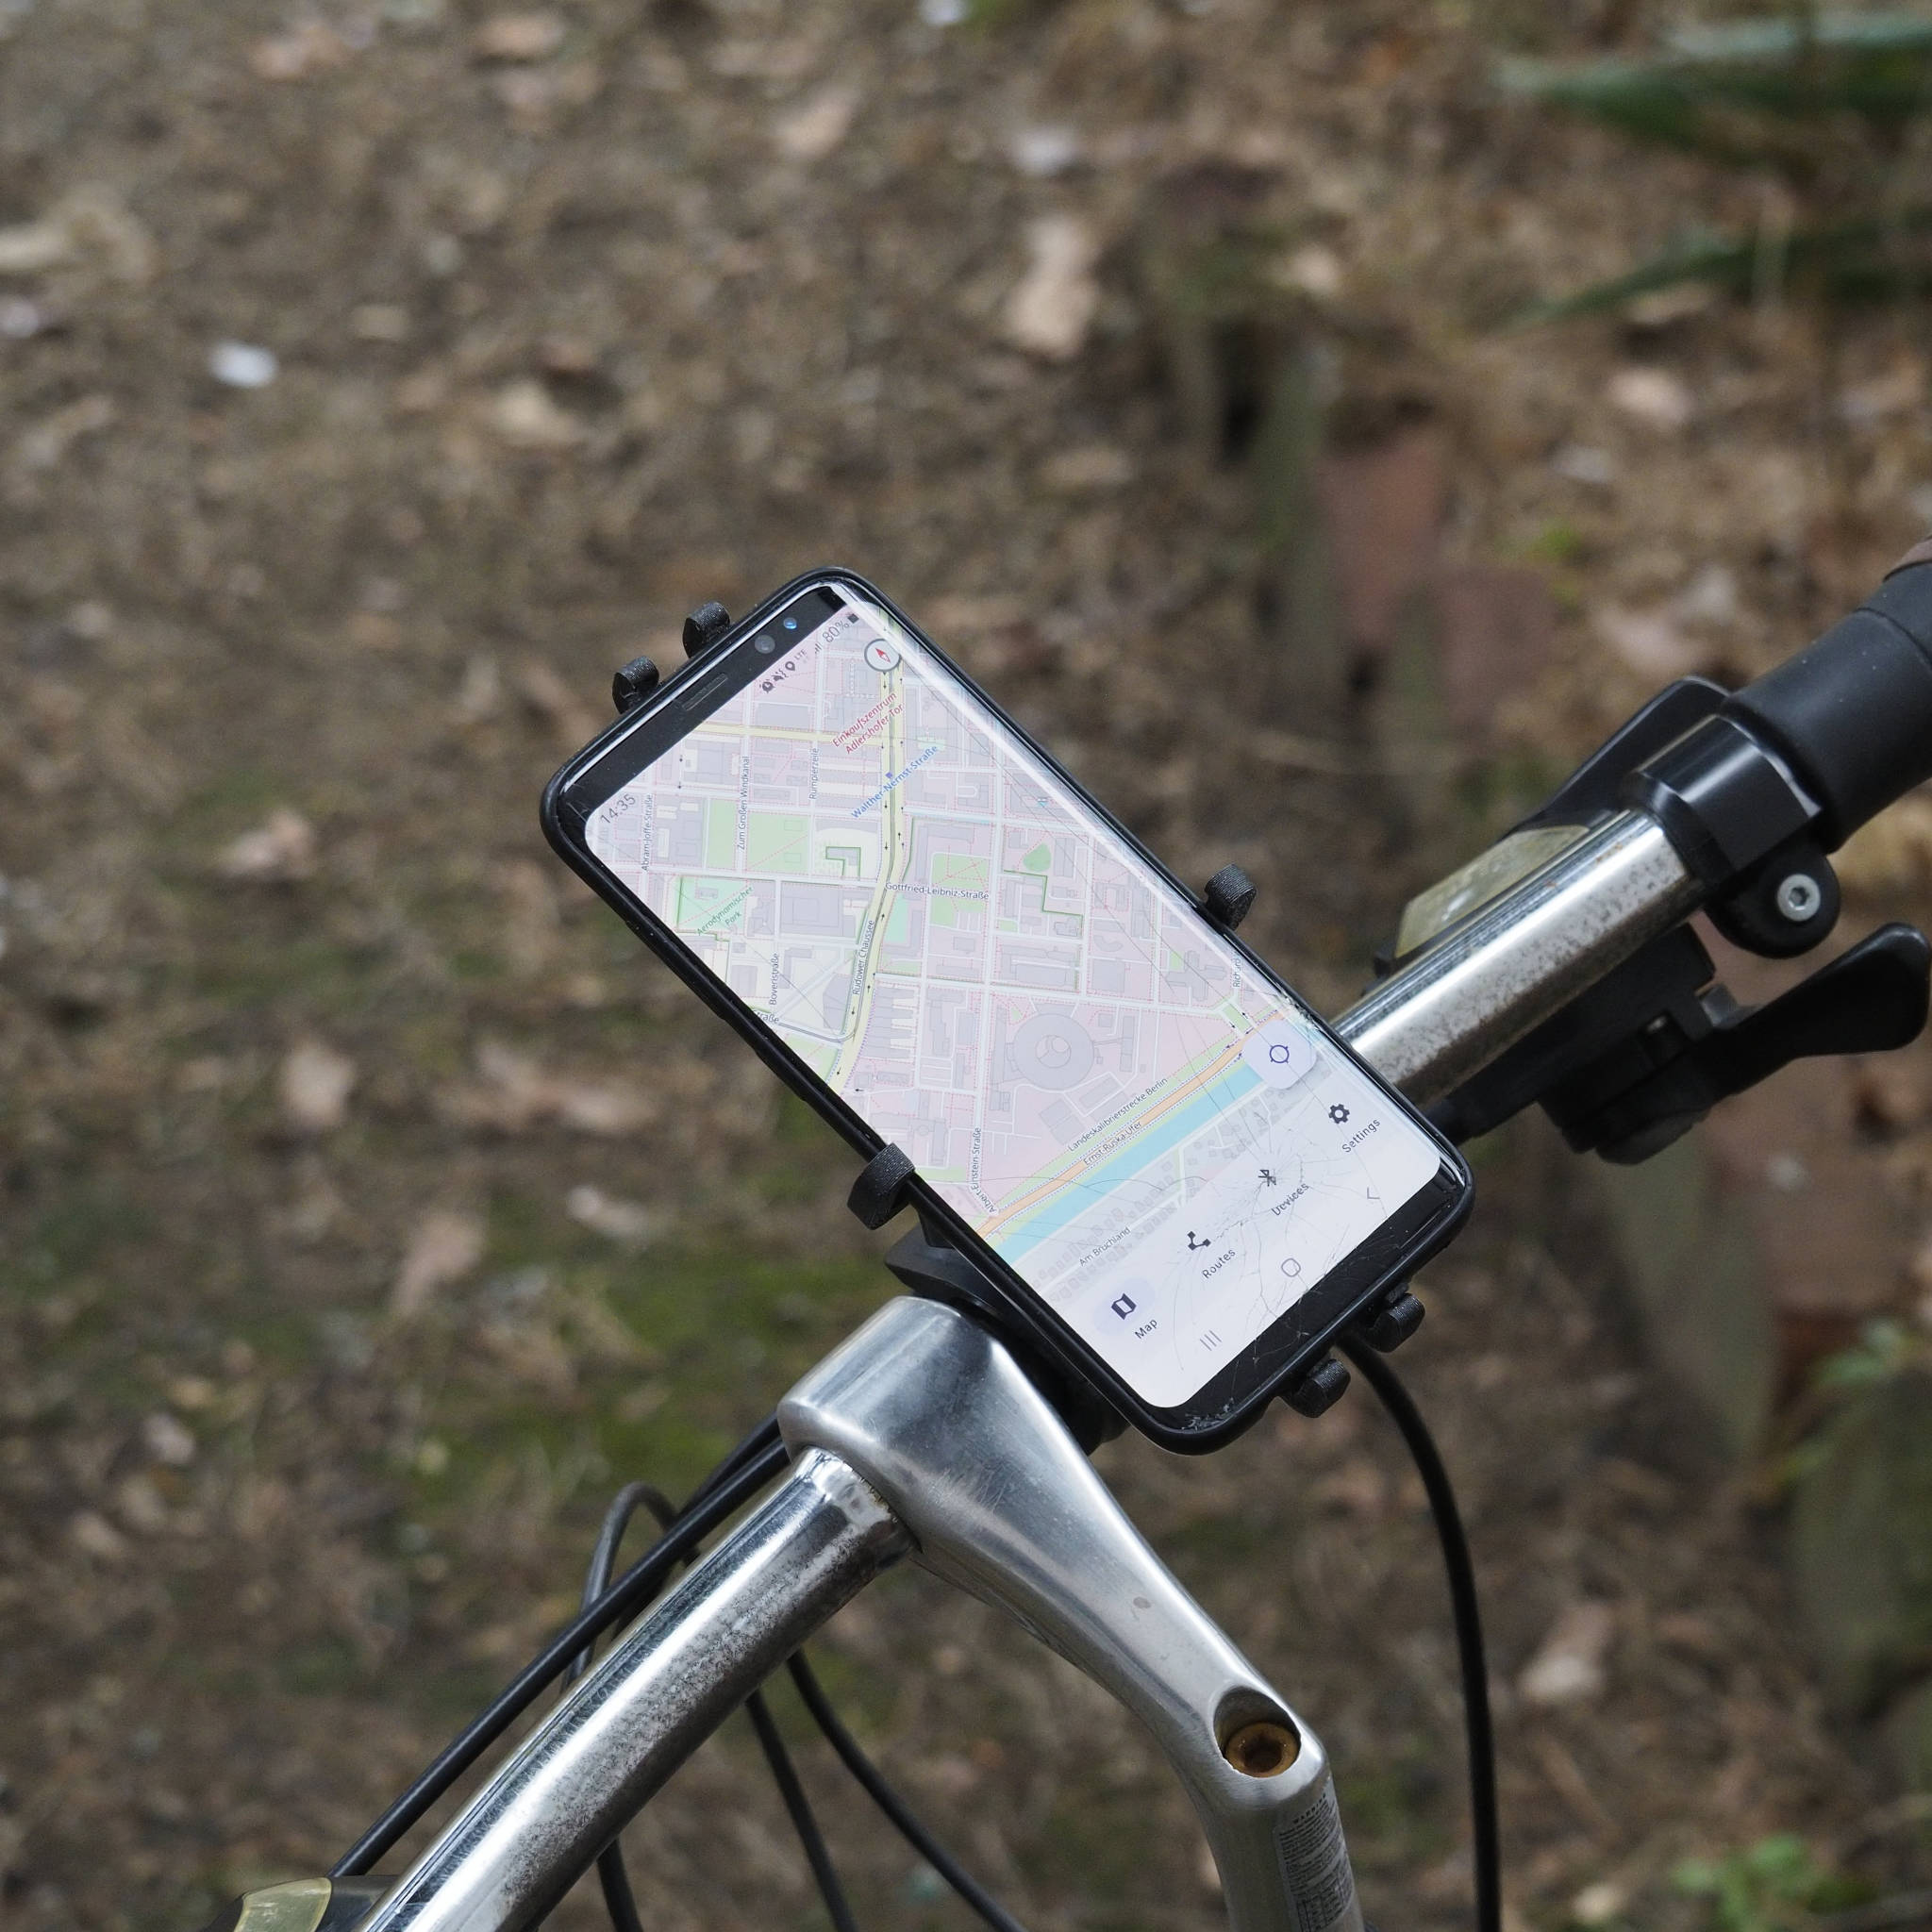
\includegraphics[width=.9229\linewidth]{images/smartphone_holder.jpg}
        \caption{Smartphone holder}
        \label{fig:smartphone_holder}
    \end{minipage}
\end{figure}

\subsubsection*{Safety Precautions}

To ensure each participants' safety, the researcher conducting the study followed them on their routes, retaining a safe distance, with another bicycle.
Participants were further told to not look at the route on the smartphone for extended periods of time and to focus their attention on the road in front of them and to stop and get in contact with the researcher if a problem occurred, but to otherwise ignore them.
They were also told to only drive at a conservative, safe speed.

\newpage\section{Results}\label{sec:results}

\subsection{Participants}

We recruited a total of 18 participants for our study using posters we placed on the university campus in combination with snowball sampling.
Participants age ranged from 18 to 59 years.
Only 3 of the 18 participants identified as female, all others identified as male.
Each participant received a compensation of \euro10.00 for their efforts.
The study was conducted from November to December, but except for temperature differences and some light rain, general weather conditions were consistent between study sessions.
Each session took about 90 minutes in total.
We experienced no study cancellations, and all recorded data was usable.

\subsection{Route Data}

In this section, we describe the evaluation of the quantitative ratings performed by participants on the measure of “Travel satisfaction, based on the road” using the \likertshift, \audiorecording, and \mapping methods respectively, as described in \autoref{subsec:recording_methods} and \autoref{subsec:data_collection}. \autoref{fig:route_ratings} shows a visually appealing overview of all data collected using all three methods.

\begin{figure}[!htb]
    \centering
    \begin{subfigure}{.3333\textwidth}
        \centering
        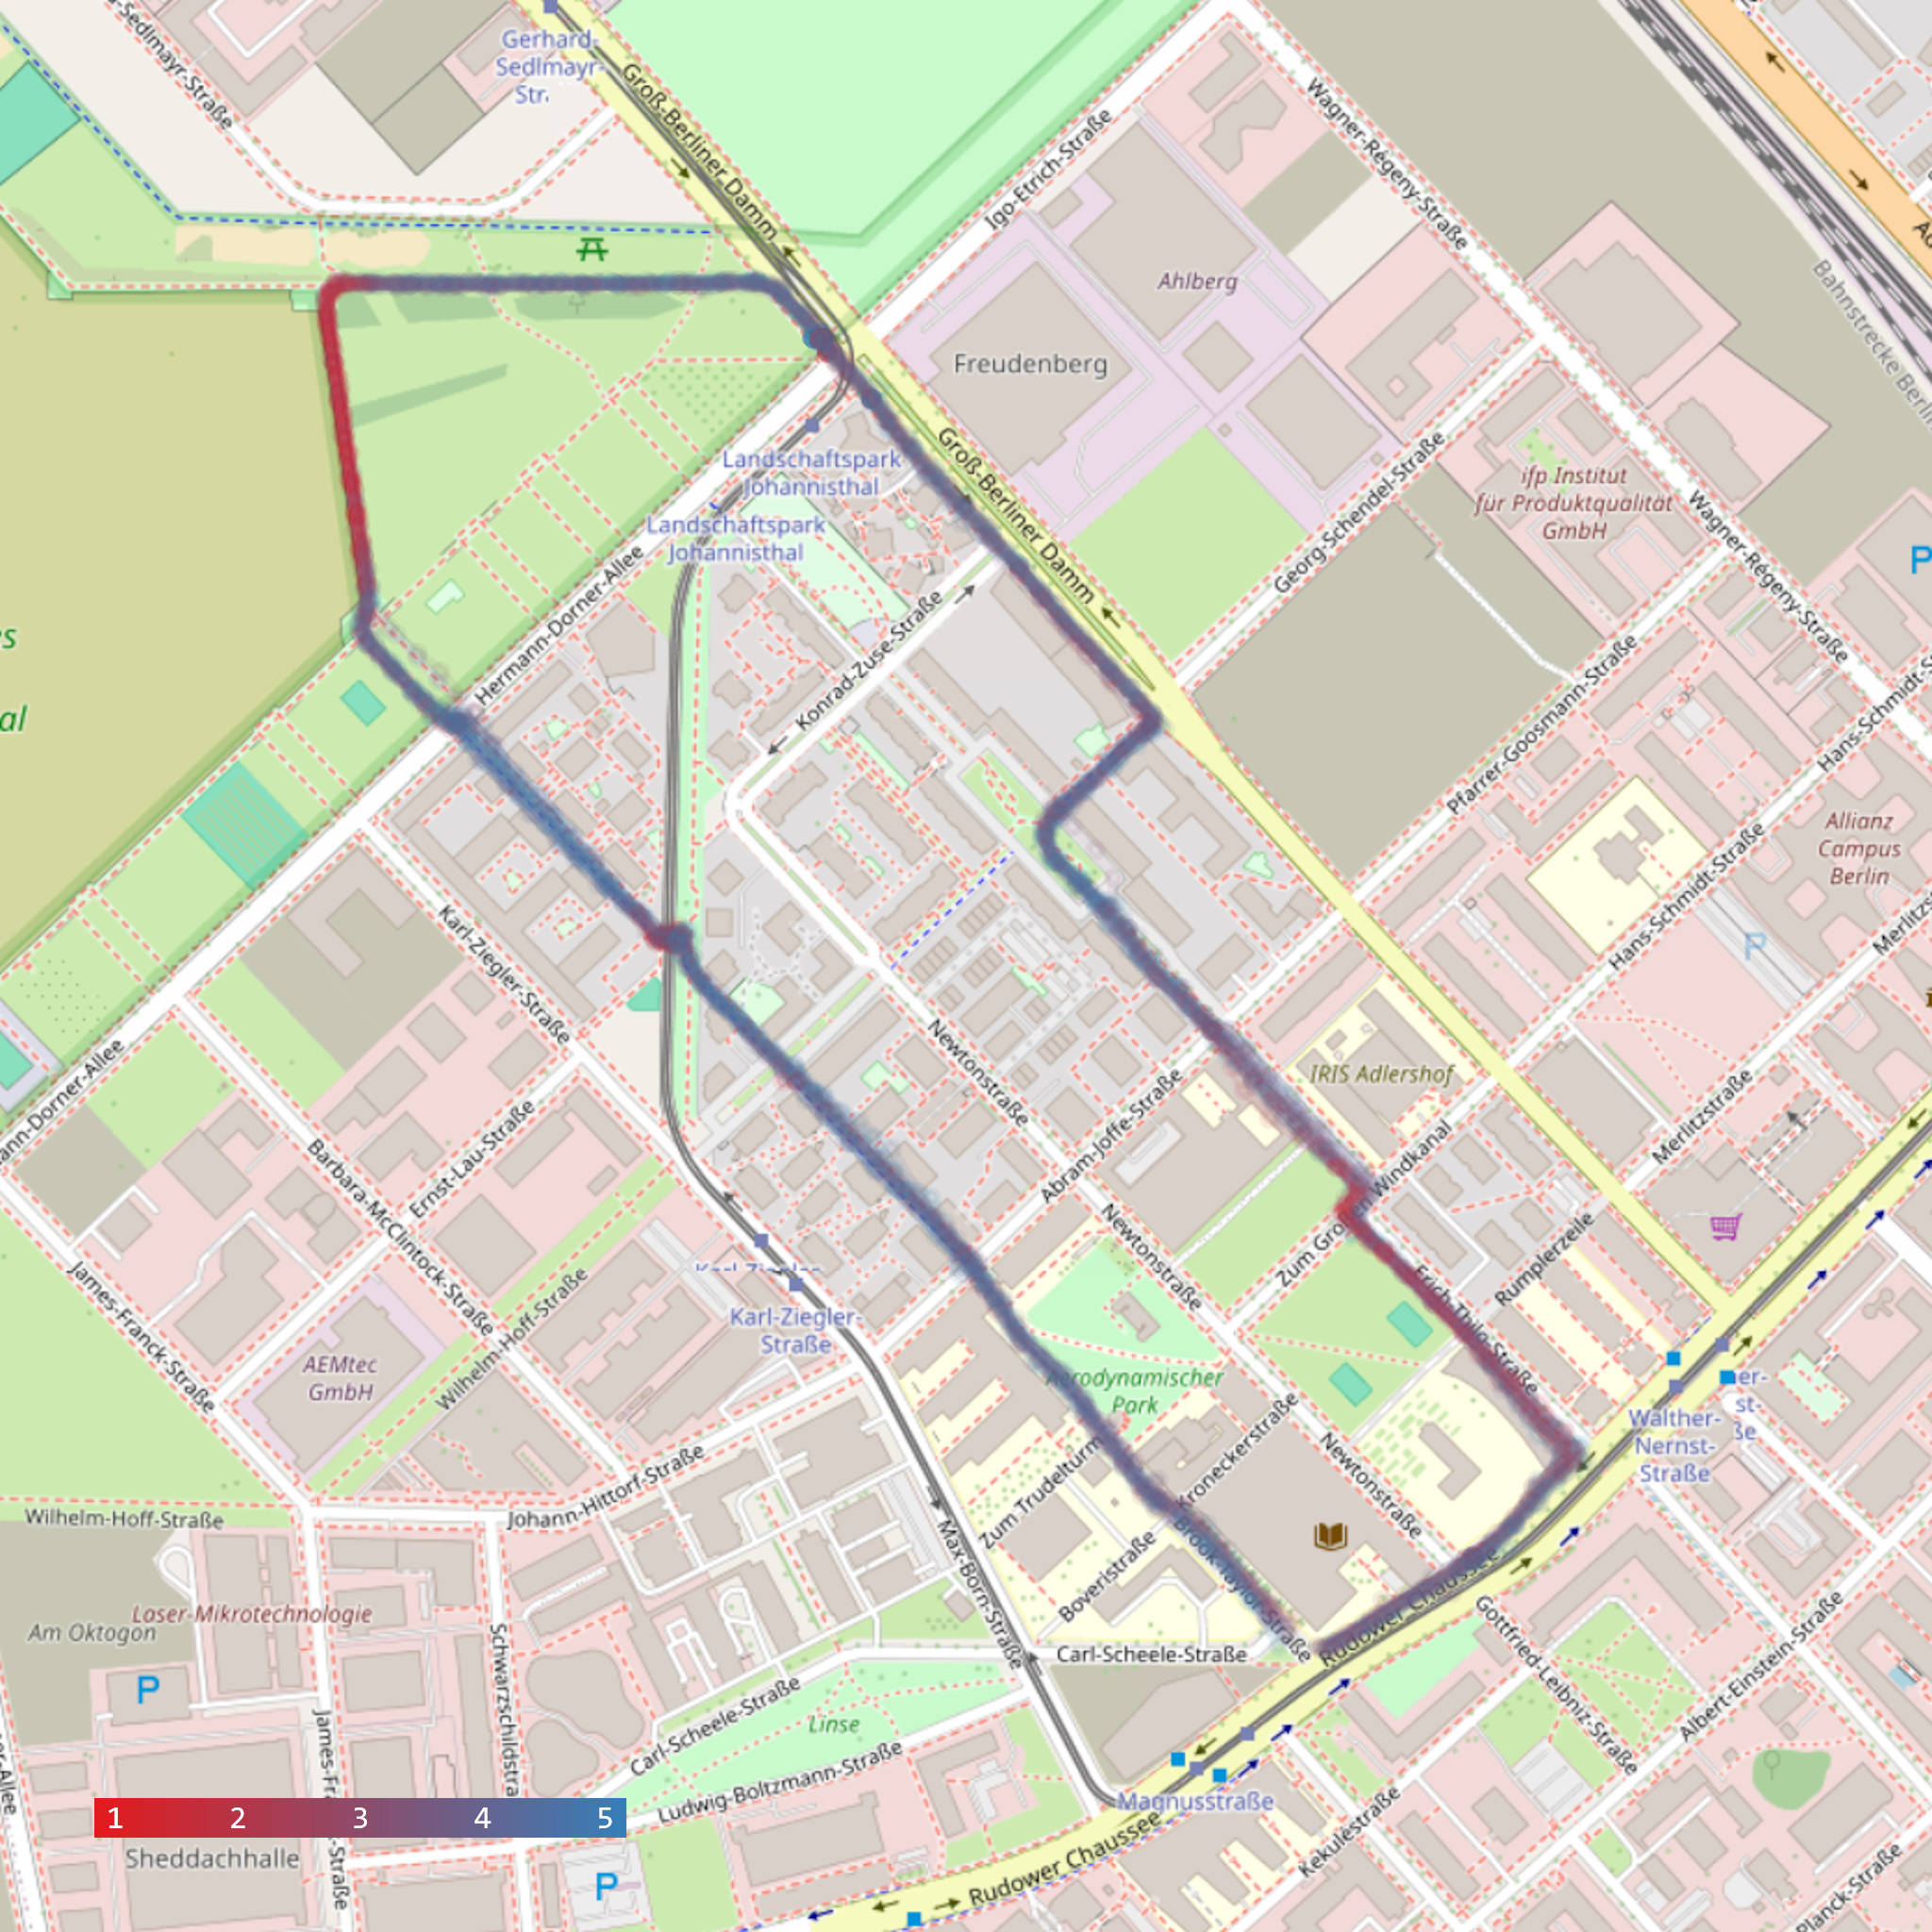
\includegraphics[width=.9\linewidth]{images/ratings_north_route.jpg}
        \caption{North route}
        \label{fig:ratings_north_route}
    \end{subfigure}%
    \begin{subfigure}{.3333\textwidth}
        \centering
        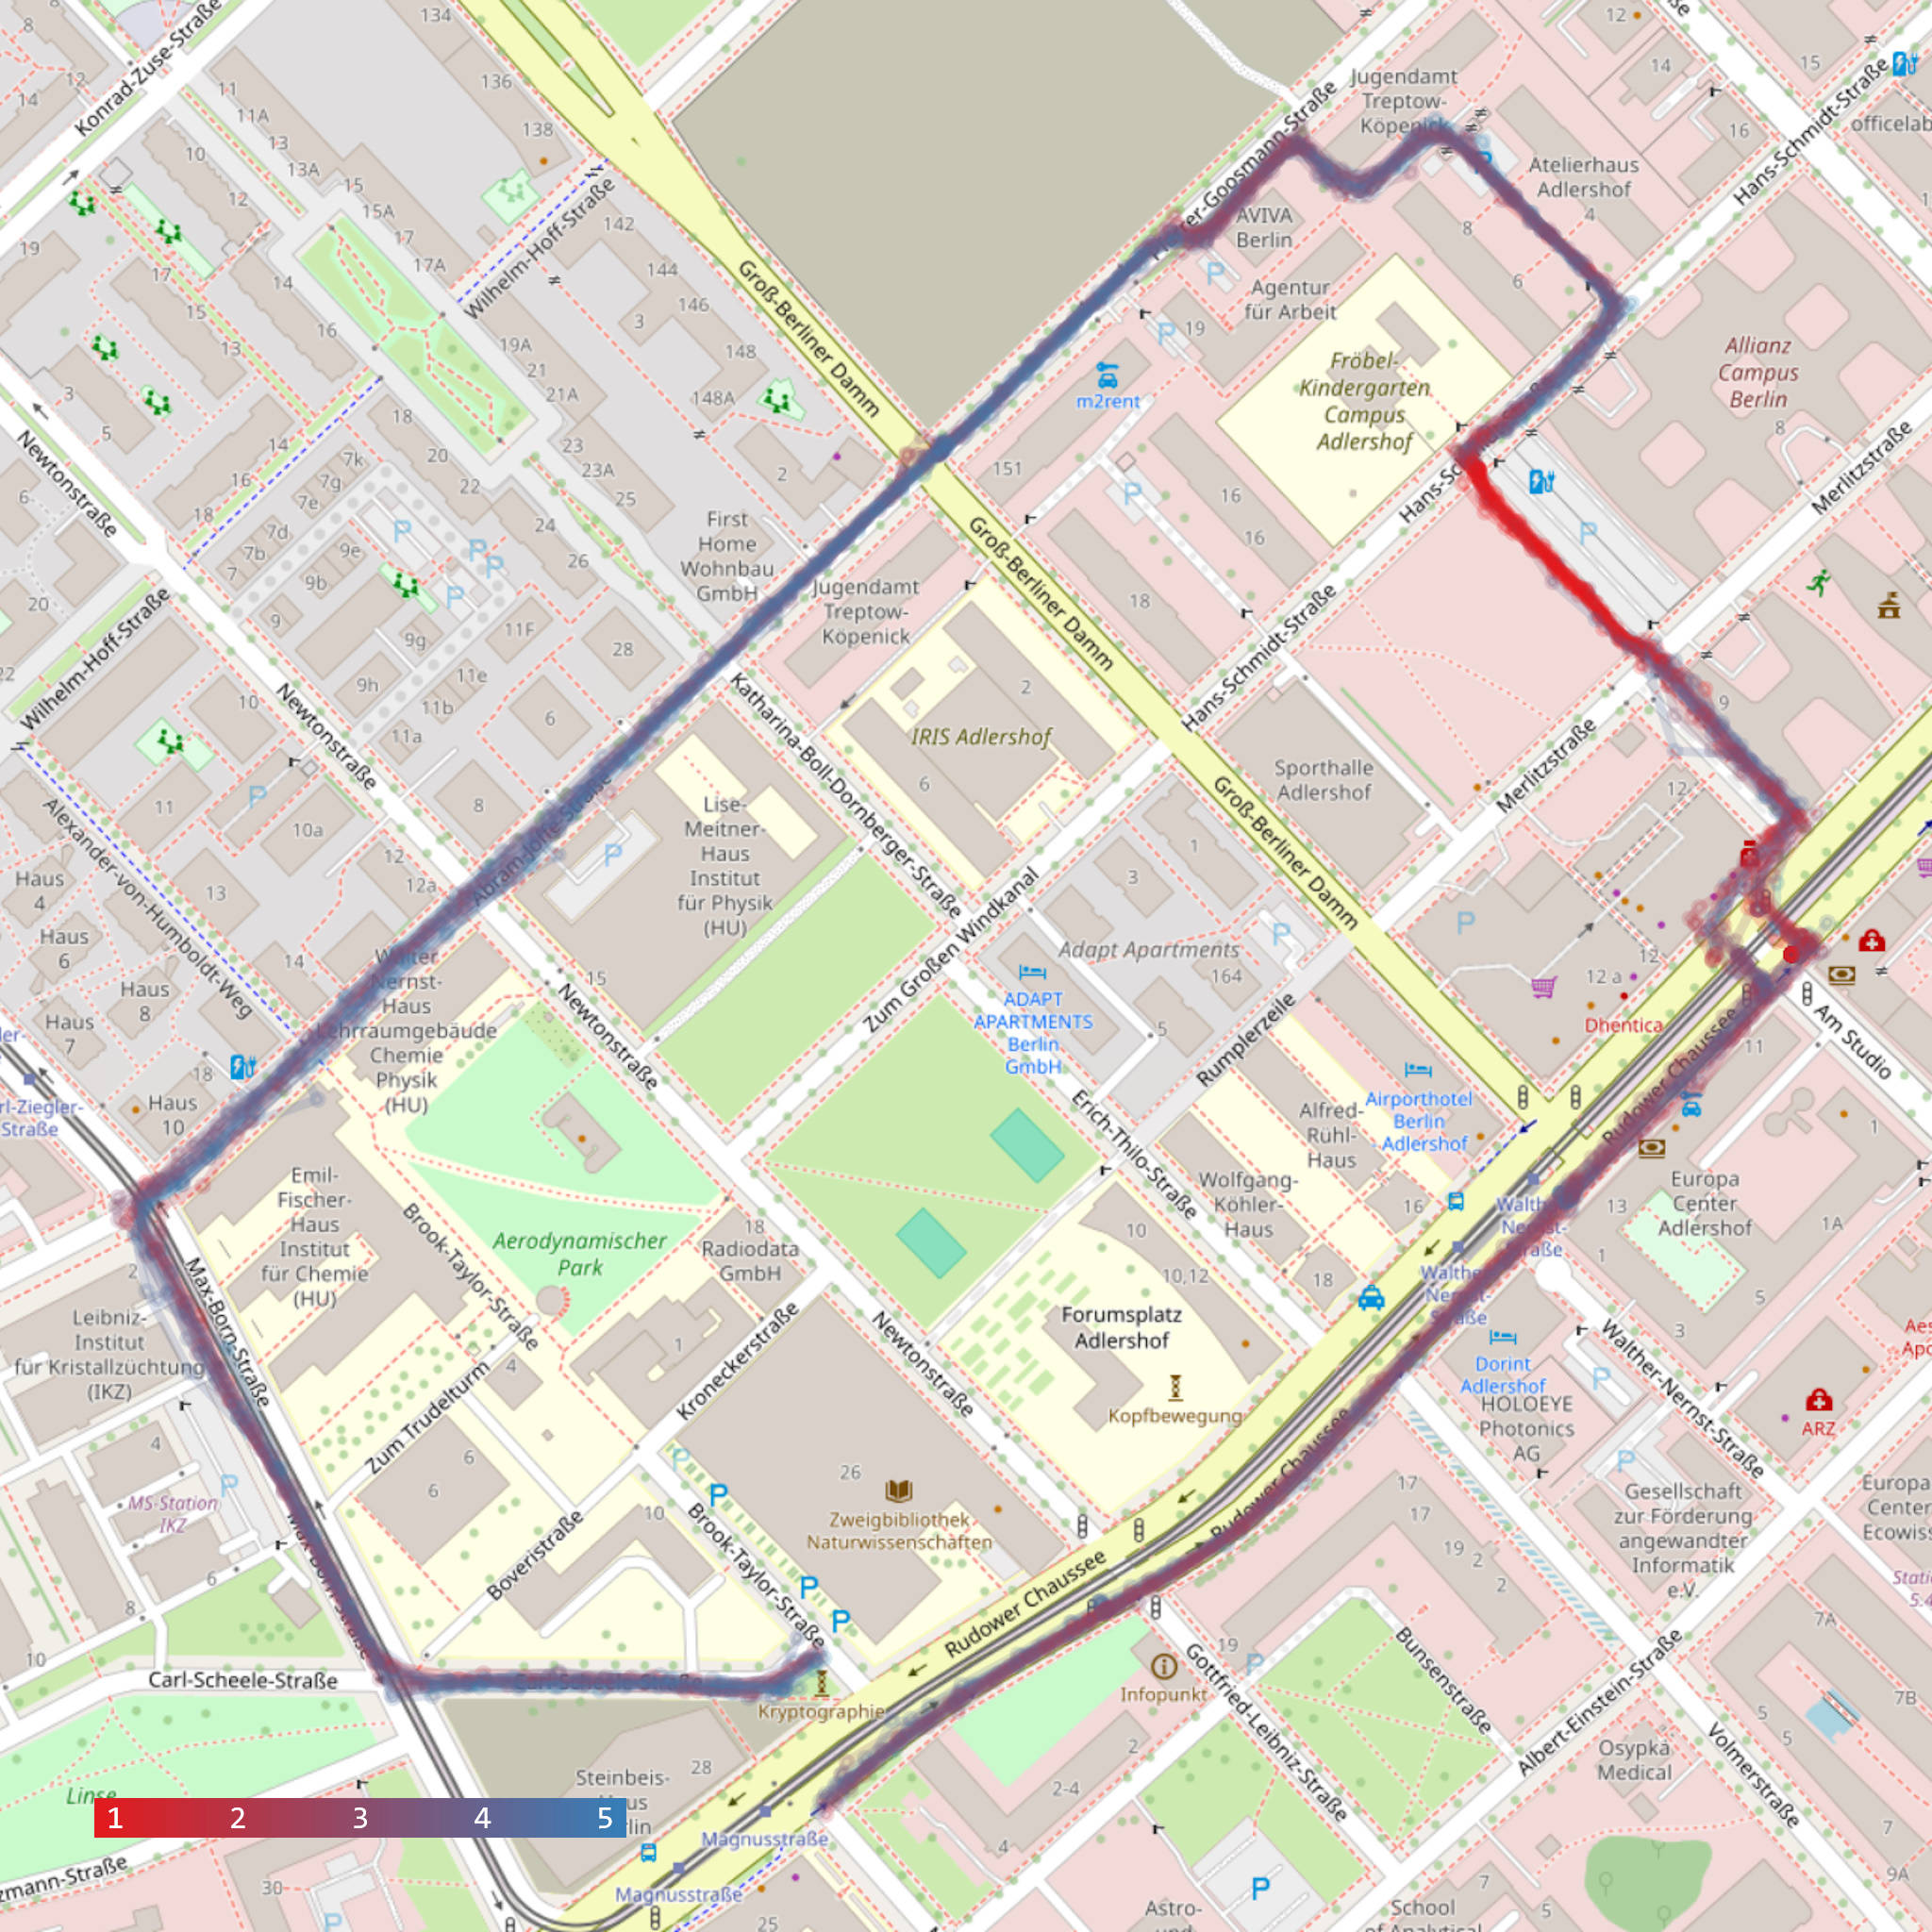
\includegraphics[width=.9\linewidth]{images/ratings_east_route.jpg}
        \caption{East route}
        \label{fig:ratings_east_route}
    \end{subfigure}%
    \begin{subfigure}{.3333\textwidth}
        \centering
        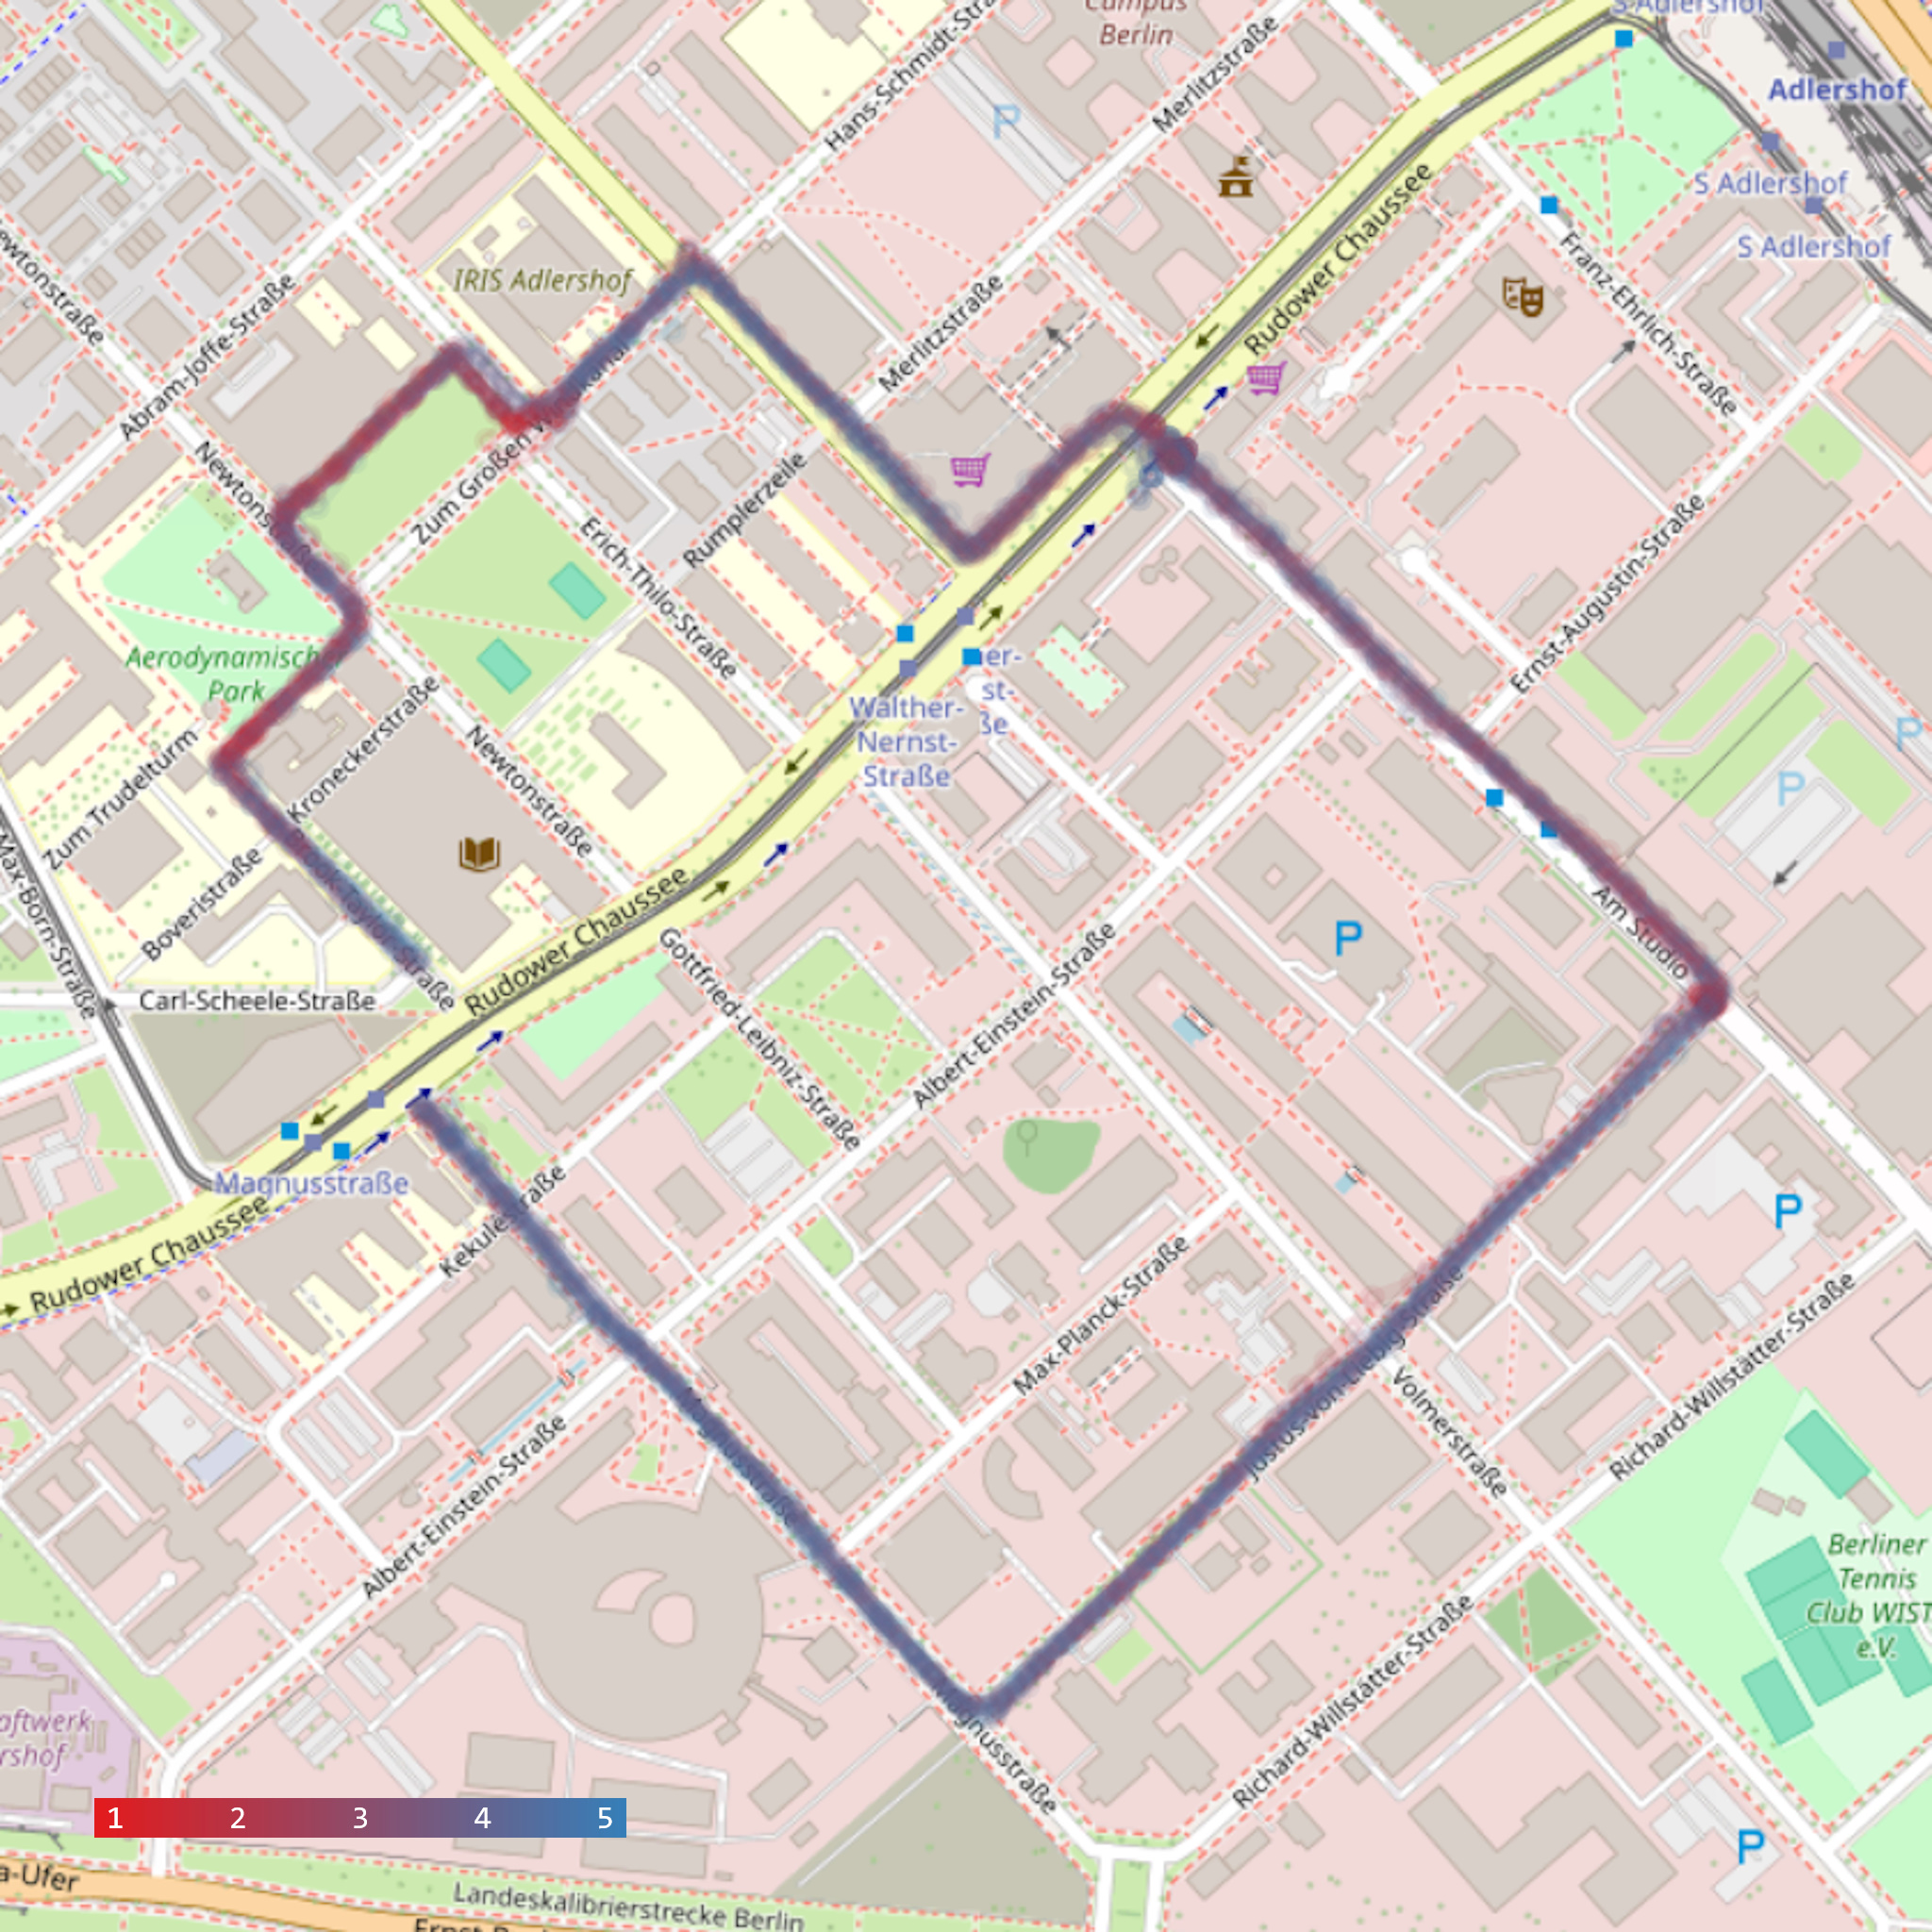
\includegraphics[width=.9\linewidth]{images/ratings_south_route.jpg}
        \caption{South route}
        \label{fig:ratings_south_route}
    \end{subfigure}\
    \caption{Combined ratings from all methods}
    \label{fig:route_ratings}
\end{figure}

\subsubsection{Preprocessing}\label{subsec:preprocessing}

Preprocessing of the recorded data was largely performed by hand, with the help of some simple Python scripts.
The start and end positions of all data recordings were adjusted manually, to remove unneeded data.
For the \audiorecording method, we had to manually listen to each audio file and extract the ratings performed by participants to match them to the recorded timestamps and GPS locations.
A similar process was used for the \mapping method to match the sections drawn on the paper maps to the recorded data.
Our \likertshift method required no further preprocessing.

\subsubsection{Evaluation}

As mentioned in \autoref{subsec:recording_methods}, comparing subjective data is inherently hard.
To perform our analysis, we categorized our original reference routes by road type and resampled them to $\sim\SI{1}{m}$ segments.
Then, we projected all recorded data from each method to them.
This left us with a combination of rating and road-type for each $\SI{1}{m}$ segment of each recording.
We then gathered all ratings by road-type for each method and computed their mean value, variance, and standard deviation, to see if we could see any drastic differences (see \autoref{table:likertshift_eval}).

\begin{table}[!htb]
    \footnotesize
    \centering
    \begin{tabular}{l|ccccccc}
        \multirow{2}{*}{\likertshift} & \multicolumn{7}{c}{Road Type}\\
        \cline{2-8}
        &&&&&&&\\[-1em]
        & Road & Bike Path & Mixed Path & Pedestrian Way & Wood Path & Field & Lawn\\[0.15em]
        \hline
        &&&&&&&\\[-0.8em]
        MEAN     & 3.7661 & 3.4624 & 3.7708 & 3.0176 & 1.8114 & 1.9804 & 2.8664\\[0.3em]
        VARIANCE & 0.9327 & 0.9140 & 0.8548 & 0.8873 & 0.9661 & 1.2512 & 1.3830\\[0.3em]
        STDDEV   & 0.9658 & 0.9560 & 0.9246 & 0.9420 & 0.9829 & 1.1186 & 1.1760\\
    \end{tabular}

    \vspace{1em}
    \begin{tabular}{l|ccccccc}
        \textsf{Audio} & \multicolumn{7}{c}{Road Type}\\
        \cline{2-8}
        &&&&&&&\\[-1em]
        \textsf{Recording} & Road & Bike Path & Mixed Path & Pedestrian Way & Wood Path & Field & Lawn\\[0.15em]
        \hline
        &&&&&&&\\[-0.8em]
        MEAN     & 3.6622 & 3.4978 & 3.7915 & 2.9559 & 2.5513 & 1.6895 & 2.4405\\[0.3em]
        VARIANCE & 0.8519 & 0.7970 & 0.8172 & 1.4158 & 0.5622 & 1.2402 & 0.9290\\[0.3em]
        STDDEV   & 0.9230 & 0.8927 & 0.9040 & 1.1899 & 0.7498 & 1.1137 & 0.9638\\
    \end{tabular}

    \vspace{1em}
    \begin{tabular}{l|ccccccc}
        \multirow{2}{*}{\mapping} & \multicolumn{7}{c}{Road Type}\\
        \cline{2-8}
        &&&&&&&\\[-1em]
        & Road & Bike Path & Mixed Path & Pedestrian Way & Wood Path & Field & Lawn\\[0.15em]
        \hline
        &&&&&&&\\[-0.8em]
        MEAN     & 3.7476 & 3.4952 & 3.7230 & 3.3553 & 2.3586 & 1.0000 & 3.0291\\[0.3em]
        VARIANCE & 0.9192 & 1.0542 & 1.0379 & 1.2773 & 1.5566 & 0.0000 & 1.0891\\[0.3em]
        STDDEV   & 0.9587 & 1.0267 & 1.0188 & 1.1302 & 1.2476 & 0.0000 & 1.0436\\
    \end{tabular}
    \caption{Evaluation of the recorded quantitative data}
    \label{table:likertshift_eval}
\end{table}

\subsection{Questionnaires and Interviews}

We evaluated each component of the \citetextnoref{nasa_tlx}{TLX} and \citetextnoref{ueq+}{UEQ+} surveys separately, without computing an overall index, because we are most interested in what components cause increased task load or affect the user experience.

The \textit{Physical Demand}, \textit{Temporal Demand}, and \textit{Performance} metrics of the \citetextnoref{nasa_tlx}{TLX} showed little statistical evidence for differences between methods.
The most notable difference is the increased \textit{Mental Demand} observed with the \mapping method, as well as higher \textit{Frustration} and perceived \textit{Effort} in comparison to the live-recording methods.
There is insufficient statistical evidence for differences in task load between our \likertshift method and the \audiorecording method.

\begin{figure}[!htb]
    \centering
    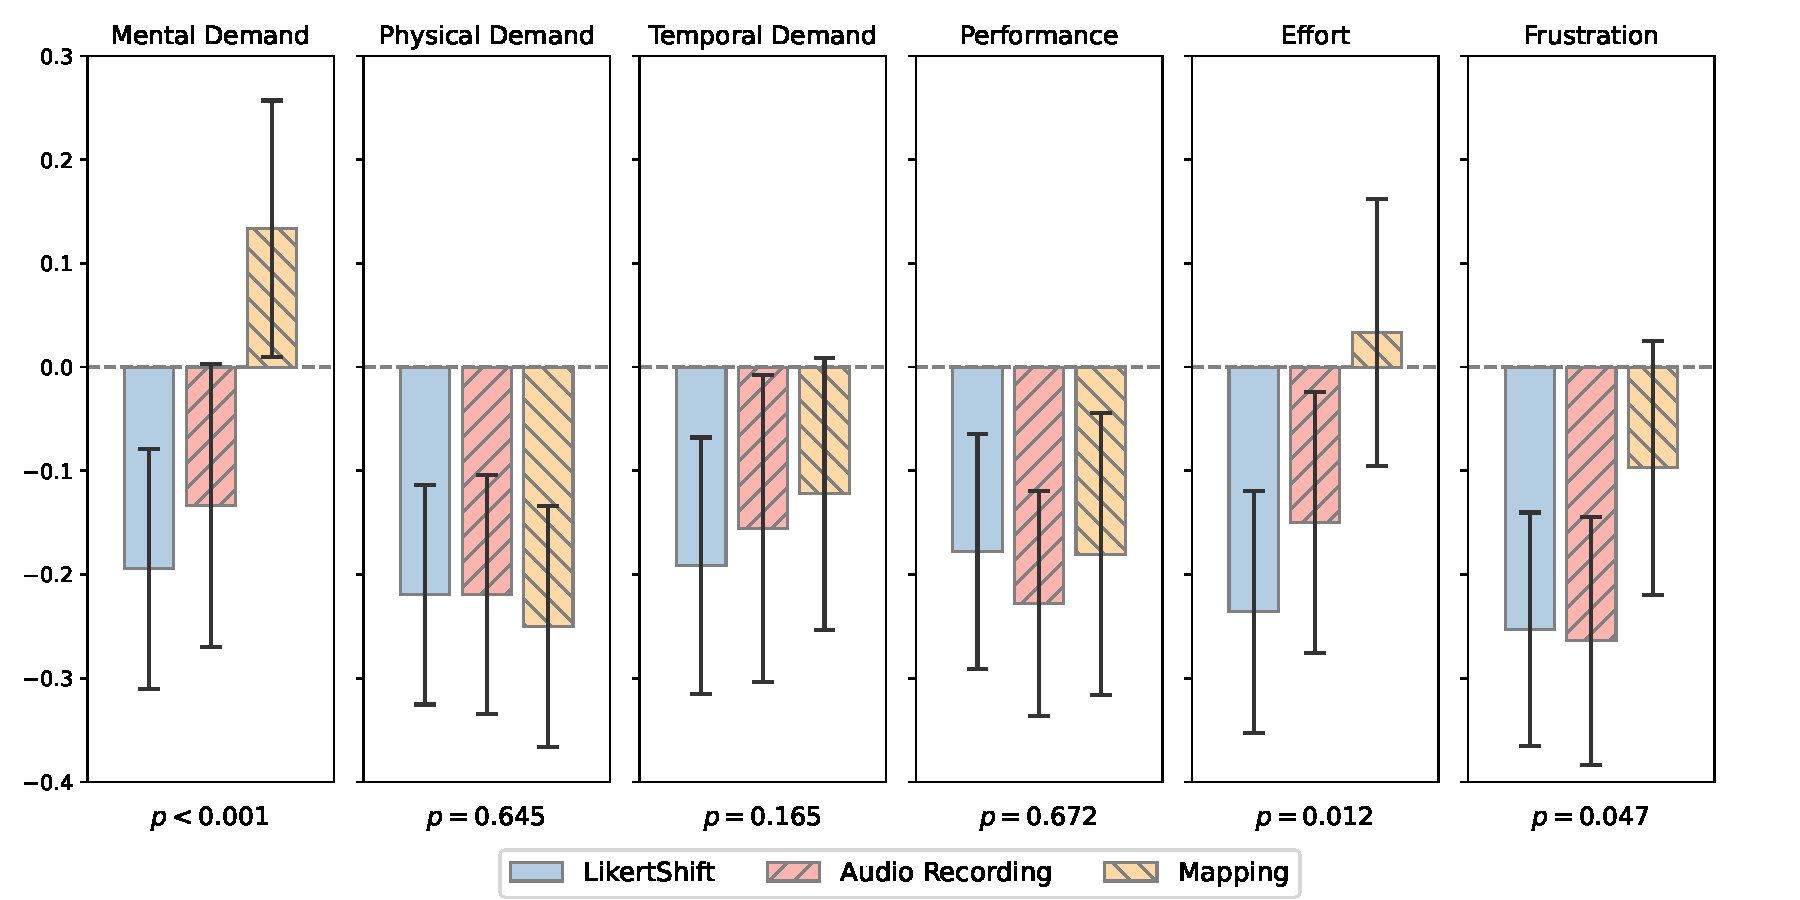
\includegraphics[height=0.5\linewidth]{../evaluation/eval_tlx.pdf}
    \caption{TLX results (error-bars denote the confidence interval based on a student's distribution; $p$ values are computed using a Friedman test; values are normalized from -1 to 1)}
    \label{fig:eval_tlx}
\end{figure}

\bigbreak\noindent
The evaluation of the \citetextnoref{ueq+}{UEQ+} metrics turned out to be more interesting.
We observed strong evidence for the \textit{Attractiveness} and \textit{Intuitiveness} of our \likertshift method, compared to the other ones.
While participants perceived the \likertshift and \audiorecording methods to be similarly \textit{Efficient}, in comparison, the \mapping method was perceived as highly inefficient.
We can also observe low \textit{Social Acceptance} ratings of the \audiorecording method.

These findings were confirmed by our performed interviews.
Multiple participants noted that the additional time requirements of the \mapping method make using it very unattractive to them.
Similarly, the majority of participants stated they did not like to talk during cycling and found it “awkward” to perform the \audiorecording method.
When asked what method participants would choose to conduct a longer ($\sim\SI{2}{weeks}$) field-study which would require them to record their travel satisfaction on all of their commutes and other trips, 17 out of 18 participants chose our \likertshift method.

\begin{figure}[!htb]
    \centering
    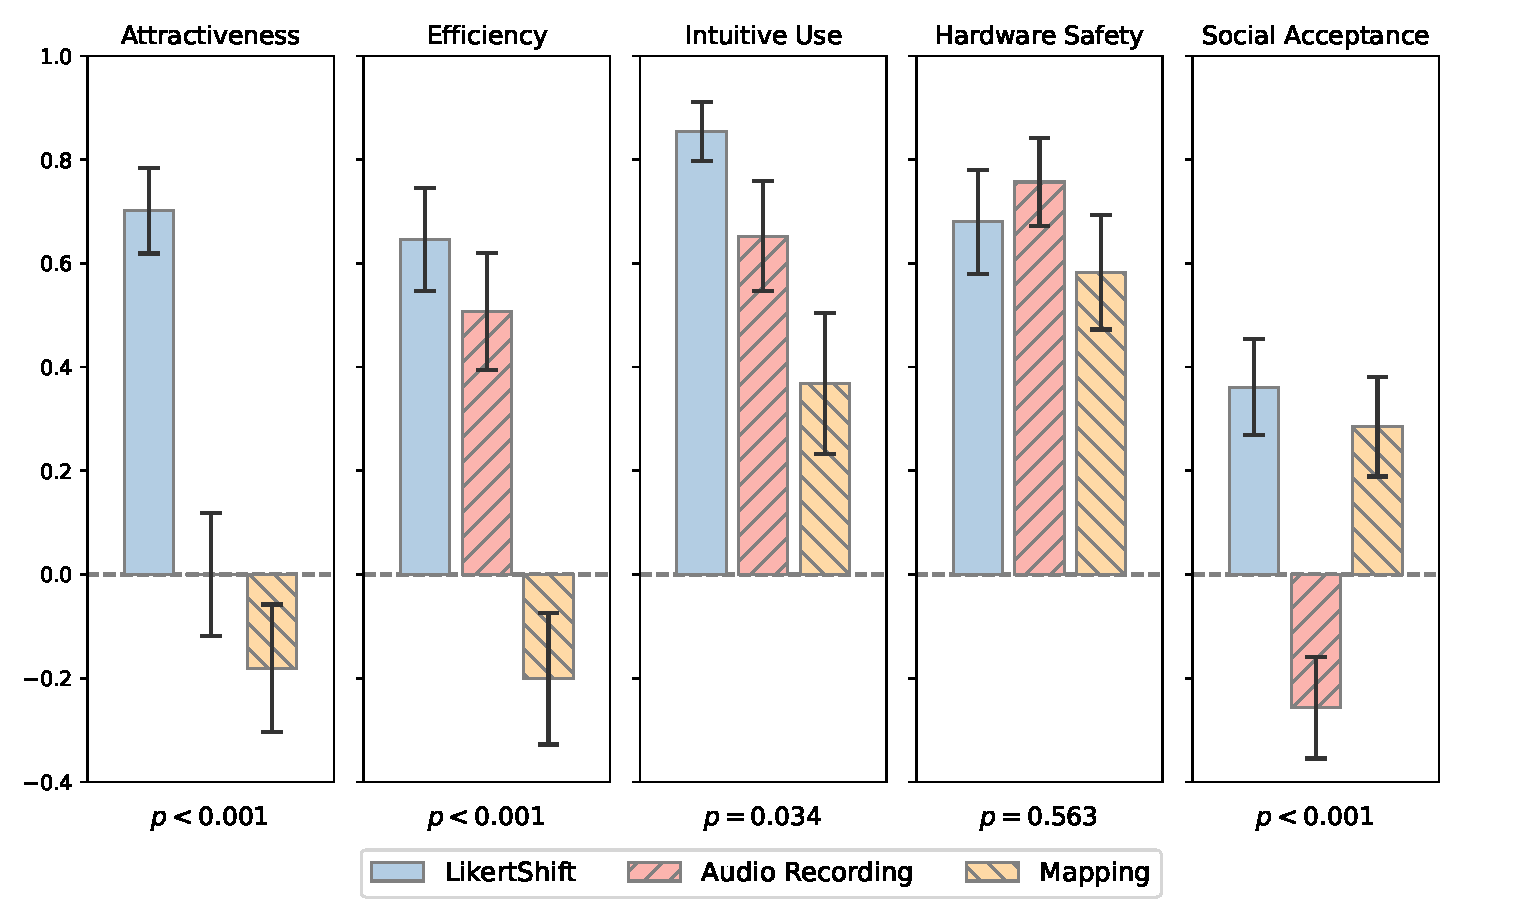
\includegraphics[height=0.5\linewidth]{../evaluation/eval_ueq.pdf}
    \caption{UEQ+ results (error-bars denote the confidence interval based on a student's distribution; $p$ values are computed using a Friedman test; values are normalized from -1 to 1)}
    \label{fig:eval_ueq}
\end{figure}

\newpage\section{Discussion}\label{sec:discussion}

\subsection{Research Questions}

\subsubsection{Q1: How do different methods to record cyclists' subjective experiences affect their
rating behavior?}

We failed to answer this question, as the evaluation of the quantitative data we recorded did not allow us to perceive any large differences.
Our best guess is that quantitative differences between methods are very subtle and require larger studies to be found.

\subsubsection{Q2: What are cyclists' preferences regarding methods to record their subjective experiences?}

Users highly prefer methods that require minimal additional work and appear invisible to other traffic participants.
While none of the methods we compared appear as particularly disturbing, especially to the users' ability to stay in control and cycle safely, \audiorecording was perceived as unpleasant, while the \mapping method exerted a higher mental demand on them.

\subsection{Future Work}

Future work could include the combination of multiple methods for recording \CSE, most notably hybrid methods, which rely on real-time data acquisition during cycling, but allow for modification after data collection is complete.
The easiest implementation of this would involve combining our \likertshift method with an adjustable map included in the smartphone app, similar to the \mapping method, but in a digital form.
This would allow for corrections, in situations where users performed rating too late or forgot them altogether.
Other improvements include the addition of active feedback to the device, for example, in the form of vibrations or sound.
This would allow for an even more intuitive rating process.
Finally, more sensors and connectivity options could be added to our \likertshift device, to make it usable standalone, without requiring a smartphone to actively record the data.

\newpage\section{Conclusion}\label{sec:conclusion}

In this work, we described the successful design and construction of the \likertshift, a prototype device that can be used to record cyclists' subjective experiences, as well as its evaluation against other state-of-the-art methods in a semi-naturalistic field-study.
Although quantitative analysis of recorded data revealed little to no statistical evidence supporting a measurable improvement in data quality using our developed \likertshift method, qualitative assessments of participants' opinions regarding the different methods provided valuable insights.
They highlighted the perceived attractiveness, intuitiveness, and efficiency of using our physical device.
Participants also voiced concerns about the social acceptance of speech recording during cycling and the high effort and increased mental demand associated with retrospective mental mapping approaches that rely on the memorization of route segments, particularly for longer routes.
From our collected evidence, we see great potential in using physical devices for recording data on cyclists' subjective experiences, especially in longer, more naturalistic field-studies.


%%%%%%%%%%%%%%%%%%%%%%%%%%%%%%%%%%%_BIBLIOGRAPHY_%%%%%%%%%%%%%%%%%%%%%%%%%%%%%%%%%%%
% create your bibliography based on your files in library/...
% remember to edit \addbibresource in the TEMPLATE_PACKAGSES area above!
\newpage
\pagenumbering{roman} % start roman page numbers from here (optional)
\bibliographystyle{abbrvurl}
\bibliography{references.bib}
%%%%%%%%%%%%%%%%%%%%%%%%%%%%%%%%%%%%%_APPENDIX_%%%%%%%%%%%%%%%%%%%%%%%%%%%%%%%%%%%%
%\newpage
%\section*{Appendix} \label{Appendix}
%\addcontentsline{toc}{section}{Appendix}    % adds entry to table of contents
%\selbstaendigkeitserklaerung{25. Januar 2025}
%\input{chapters/xxx}                       % add in case you have additional images/tables
\end{document}
%%%%%%%%%%%%%%%%%%%%%%%%%%%%%%%%%%%%%%%%%%%%%%%%%%%%%%%%%%%%%%%%%%%%%%%%%%%%%%%%%%%%
